%!TEX program = xelatex
%\documentclass[authoryear,12pt]{book}
%\usepackage{xeCJK}
%\setCJKmainfont[BoldFont={SimHei}]{SimSun}
%\setCJKsansfont{SimHei}
%\setCJKmonofont{[simfang.ttf]}
%\setCJKfamilyfont{zhsong}{SimSun}
%\setCJKfamilyfont{zhhei}{SimHei}
%\setCJKfamilyfont{zhfs}{[simfang.ttf]}

%\documentclass[UTF8,adobefonts]{ctexbook} % 采用Adobe字体
\documentclass[10pt,a4paper,twoside,openright,UTF8]{ctexbook} % 采用Adobe字体
%10pt,a4paper,twoside,openright,titlepage,fleqn,               headinclude,,footinclude,BCOR5mm,numbers=noenddot,cleardoublepage=empty,               tablecaptionabove, UTF8


\pagestyle{plain}

%% Use the option review to obtain double line spacing
%% \documentclass[authoryear,preprint,review,12pt]{elsarticle}

%% Use the options 1p,twocolumn; 3p; 3p,twocolumn; 5p; or 5p,twocolumn
%% for a journal layout:
%% \documentclass[final,authoryear,1p,times]{elsarticle}
%% \documentclass[final,authoryear,1p,times,twocolumn]{elsarticle}
%% \documentclass[final,authoryear,3p,times]{elsarticle}
%% \documentclass[final,authoryear,3p,times,twocolumn]{elsarticle}
%% \documentclass[final,authoryear,5p,times]{elsarticle}
%% \documentclass[final,authoryear,5p,times,twocolumn]{elsarticle}

%% if you use PostScript figures in your article
%% use the graphics package for simple commands
%% \usepackage{graphics}
%% or use the graphicx package for more complicated commands
 \usepackage{graphicx}
%% or use the epsfig package if you prefer to use the old commands
%% \usepackage{epsfig}

%% The amssymb package provides various useful mathematical symbols
\usepackage{amssymb}
%% The amsthm package provides extended theorem environments
\usepackage{amsmath, amsthm}

%% The numcompress package shorten the last page in references.
%% `nodots' option removes dots from firstnames in references.
\usepackage[nodots]{numcompress}
\usepackage{url}
\usepackage{hyperref}
\usepackage{threeparttable}
\usepackage{multirow}
\usepackage{natbib}
%\usepackage[backend=biber,style=numeric-comp]{biblatex}
%% The lineno packages adds line numbers. Start line numbering with
%% \begin{linenumbers}, end it with \end{linenumbers}. Or switch it on
%% for the whole article with \linenumbers after \end{frontmatter}.
\usepackage{lineno}
\usepackage[titletoc]{appendix}
%% natbib.sty is loaded by default. However, natbib options can be
%% provided with \biboptions{...} command. Following options are
%% valid:

%% round  -  round parentheses are used (default)
%% square -  square brackets are used   [option]
%% curly  -  curly braces are used      {option}
%% angle  -  angle brackets are used    <option>
%% semicolon  -  multiple citations separated by semi-colon (default)
%% colon  - same as semicolon, an earlier confusion
%% comma  -  separated by comma
%% authoryear - selects author-year citations (default)
%% numbers-  selects numerical citations
%% super  -  numerical citations as superscripts
%% sort   -  sorts multiple citations according to order in ref. list
%% sort&compress   -  like sort, but also compresses numerical citations
%% compress - compresses without sorting
%% longnamesfirst  -  makes first citation full author list
%%

% \biboptions{}
%\usepackage[nolists]{endfloat}
\usepackage{geometry}
%\geometry{left=2cm,right=2cm,top=2cm,bottom=2cm}
%\geometry{top=3cm,bottom=4cm}

\usepackage{fancyhdr}
\pagestyle{fancy}
\fancyhead[LE,RO]{\slshape \rightmark}
\fancyhead[LO,RE]{\slshape \leftmark}
\fancyfoot[C]{\thepage}




\author{朱彦元 \\ \href{mailto:yyz@tongji.edu.cn}{yyz@tongji.edu.cn}
  \\
  同济大学,中德工程学院}
\title{ DSGE模型笔记 }
%\subtitle{ (中德工程学院经济工程专业)}
\begin{document}

\maketitle
\newpage
\tableofcontents{}
\listoffigures
\listoftables
\newpage

\chapter{前言}
还没想好要写什么...
%!TEX root = ../DSGEnotes.tex
\chapter{基准New Keynesian模型}
\label{sec:Basic-NK-model}

\section{家庭部门}
\label{sec:Basic-NK-model-HH-sector}


假定cashless economy,家庭的效用函数$U(C_t, N_t)$表示为\footnote{膏按:RBC(DSGE)在经验研究中中常用工作小时数而非就业人员数作为$N_t$的代理变量,其相关讨论早期文献可见\cite{Hansen:1985ku,Rogerson:1988js};近期的综述见\cite{Rogerson:2009ez}。}
\begin{equation}
  \label{eq:utility-function}
  U(C_t, N_t) = \frac{C_t^{1-\sigma}}{1-\sigma} - \psi \cdot \frac{N_t^{1+\eta}}{1+\eta},
\end{equation}

HH问题。目标:追求效用最大化
\begin{align}
  \label{eq:HH-problem-max}
  \max_{\{C_t, N_t, B_{t+1}\}} & E_0 \sum_{t=0}^{\infty} \beta^t \cdot U(C_t, N_t), \nonumber \\
&st. \quad P_t \cdot C_t + B_{t+1} \le W_t \cdot N_t + Div_t - P_t \cdot T_t + (1+i_{t-1}) \cdot B_t,
\end{align}
其中$Div_t$表示dividends,中间产品企业的(垄断)利润。$T_t$表示税收或转移支付。$i_t$为名义利率。

建Lagrange
\begin{equation}
  \label{eq:HH-problem-lagrange}
  \mathcal{L} = E_0 \sum_{t=0}^{\infty} \beta^t \cdot \{ U(C_t, N_t) + \lambda_t \cdot \left[W_t \cdot N_t + Div_t - P_t \cdot T_t + (1+i_{t-1}) \cdot B_t - P_t \cdot C_t - B_{t+1}\right]\}.
\end{equation}

FOCs
\begin{align*}
  \frac{\partial \mathcal{L}}{\partial C_t}=0 &\Rightarrow C_t^{-\sigma} = \lambda_t \cdot P_t \\
  \frac{\partial \mathcal{L}}{\partial N_t}=0 & \Rightarrow \psi \cdot N_t^{\eta} = \lambda_t \cdot W_t \\
\frac{\partial \mathcal{L}}{\partial B_{t+1}}=0 & \Rightarrow \frac{\partial \{\lambda_t \cdot (1 + i_{t-1}) \cdot B_t\}}{\partial B_{t+1}} - \lambda_t = \frac{\partial \beta \cdot E_t \{ \lambda_{t+1} \cdot (1 + i_{t}) \cdot B_{t+1} \} } {\partial B_{t+1}} - \lambda_t = 0\\
\end{align*}

整理得
\begin{gather}
  \label{HH-FOC-labor-supply}
  \psi \cdot N_t^{\eta} = C_t^{-\sigma} \cdot w_t \\
\label{HH-FOC-euler-consumption}
  C_t^{-\sigma} = \beta \cdot E_t\{ C_{t+1}^{-\sigma} \cdot (1+i_t) \cdot \frac{P_t}{P_{t+1}}\}=\beta \cdot E_t\{ C_{t+1}^{-\sigma} \cdot (1+i_t) \cdot ( 1+\pi_{t+1} )^{-1}\},
\end{gather}
其中$w_t \equiv \frac{W_t}{P_t}$表示实际工资,$\pi_t \equiv P_t/P_{t-1}$表示通货膨胀率。由  \eqref{HH-FOC-labor-supply}可得Frisch elasticity of labor supply为$1/\eta$\footnote{假定短时期内家庭的总财富(总消费)不变,市场上工资的变化只影响家庭的劳动力供应,Frisch labor supply elasticity\citep{Frisch:1932wk,Frisch:1959jt}可表示为
  \begin{equation*}
    \frac{\partial n_t}{\partial w_t} \cdot \frac{w_t}{n_t},
  \end{equation*}
可参考\cite[pp.279]{Heer:2009ig},以及\cite{Christiano:2010wla}。}。



\section{企业部门}
\label{sec:Basic-NK-model-firm-sector}

\subsection{最终产品生产部门}
\label{sec:Basic-NK-model-final-produc-firm-sector}
最终产品部门以中间产品$Y_t(j), j \in [0,1]$的组合为投入要素,产出$Y_t$,符合完全竞争假定。\cite{Dixit:1977tv}形式的生产规模报酬不变生产函数为
\begin{equation}
  \label{eq:fin-prod-prod-func}
  Y_t = \left[ \int_{0}^{1} Y_t(j)^{\frac{\epsilon - 1}{\epsilon}} dj\right]^{\frac{\epsilon}{\epsilon - 1}},
\end{equation}
其中$\epsilon > 1$表示$j^{th}$中间产品的替代弹性。

最终产品厂商问题:在给定$P_t(j)$的情况下,通过选择$Y_t(j)$的投入追求利润最大化

\begin{equation}
  \label{eq:fin-prod-problem-max}
  \max_{Y_t(j)} P_t \cdot Y_t - \int_{0}^{1} P_t(j) \cdot Y_t(j) dj ,
\end{equation}

引入式\eqref{eq:fin-prod-prod-func},FOC整理可得对$j$中间产品的需求函数
\begin{equation}
  \label{eq:demand-for-intm-j}
  Y_t(j) = \left( \frac{P_t(j)}{P_t}
\right)^{-\epsilon} \cdot Y_t,
\end{equation}

进而根据完全竞争市场假定
\begin{equation*}
  \begin{split}
    P_t \cdot Y_t & \equiv \int_0^1 P_t(j) \cdot Y_t(j) dj \\
    &=\left[\int_0^1 \left(\frac{P_t(j)}{P_t}\right)^{-\epsilon} \cdot Y_t \cdot P_t(j) dj \right] \\
    &=\left[\int_0^1 P_t(j)^{1-\epsilon} dj \right] \cdot P_t^{\epsilon} \cdot Y_t,\\
  \end{split}
\end{equation*}
整理得最终产品价格的决定(aggregate price index):
\begin{equation}
  \label{eq:agg-price-index}
  P_t = \left[
    \int_0^1 P_t(j)^{1-\epsilon} dj
  \right]^{\frac{1}{1-\epsilon}}
\end{equation}

\subsection{中间产品生产部门}
\label{sec:Basic-NK-model-intm-produc-firm-sector}
中间产品生产部门假定处于垄断竞争状态。代表企业$j$雇佣劳动力$N_t(j)$生产$Y_t(j)$,生产函数形式
\begin{equation}
  \label{eq:intm-prodc-func}
  Y_t(j) = A_t \cdot N_t(j),
\end{equation}
其中$A_t$表示外生的生产率冲击,它对所有中间产品生产者都是相同的。对劳动力的总需求为$j$个厂商的加总。
\begin{equation}
  \label{eq:Labor-D-S}
  N_t = \int_0^1 N_t(j)dj.
\end{equation}

\subsubsection{成本最小化:边际成本与工资}
\label{sec:intm-min-cost}
中间产品生产者$j$的问题可以表示为两阶段优化。第一阶段为成本最小化:在给定工资$W_t$的基础上,选择雇佣劳动力投入$N_t(j)$,生产中间品$Y_t(j)$,以满足最终产品生产部门对$Y_t(j)$的需求,
\begin{equation}
  \label{eq:intm-prod-max-N}
  \begin{split}
      \min_{N_t(j)} &W_t \cdot N_t(j),\\
      &st. \quad A_t \cdot N_t(j) \ge \left( \frac{P_t(j)}{P_t}\right)^{-\epsilon} Y_t,
  \end{split}
\end{equation}
第二行LHS和RHS分别表示中间产品$Y_t(j)$的供应和需求,见式\eqref{eq:intm-prodc-func}和式 \eqref{eq:demand-for-intm-j}。

建Lagrange
\begin{equation*}
  \mathcal{L} = W_t \cdot N_t(j) + \lambda_t \cdot \left[
\left(\frac{P_t(j)}{P_t}\right)^{-\epsilon} \cdot Y_t - A_t \cdot N_t(j)
\right],
\end{equation*}
其中拉格朗日乘子$\lambda_t$表示$j$生产额外1单位$Y_t(j)$的影子价格(边际成本),设为$MC_t \equiv \lambda_t $.

FOC:
\begin{equation*}
  MC_t = \frac{W_t}{A_t}
\end{equation*}

或者用实际价格形式表示
\begin{equation}
  \label{eq:intm-prod-min-N-mc}
    mc_t = \frac{MC_t}{P_t} = \frac{W_t}{A_t \cdot P_t} = \frac{w_t}{A_t}.
\end{equation}

式\eqref{eq:intm-prod-min-N-mc}  反映了实际(边际成本)和实际工资的对应关系。

\subsubsection{利润最大化:定价策略}
\label{sec:intm-max-profit}
在此基础上,第二阶段,中间产品生产者$j$对自己的产品$Y_t(j)$定价$P_t(j)$,以追求实际利润$\Pi_t$最大化。
\begin{equation}
  \label{eq:intm-prod-profit}
  \begin{split}
    \Pi_t(j) &= \frac{P_t(j) \cdot Y_t(j)}{P_t} - \frac{W_t \cdot N_t(j)}{P_t} \\
    &=\frac{P_t(j)}{P_t} \cdot Y_t(j) - mc_t \cdot Y_t(j) \\
    &=\left( \frac{P_t(j)}{P_t}\right)^{1-\epsilon} \cdot Y_t - mc_t \cdot \left( \frac{P_t(j)}{P_t}\right)^{-\epsilon} \cdot Y_t
  \end{split}
\end{equation}

粘性价格。在$t$时期,中间产品生产者$j$ 有$\phi<1$的概率不能调整价格,维持上一期的定价$P_{t-1}(j)$;有$1-\phi$的概率可以调整价格,将产品售价更新为$P_t^{\#}(j)$。
\begin{equation}
  \label{eq:intm-stick-prices}
  P_t(j) =
  \begin{cases} P_{t-1}(j) &\mbox{with prob.} \quad \phi \\
    P_t^{\#}(j) & \mbox{else} \quad 1-\phi
\end{cases}
\end{equation}

根据模型假设,中间产品生产部门由于垄断产生的利润$\Pi_t$,流回到家庭部门,供消费以提升效用,满足跨期消费的Euler equation式\eqref{HH-FOC-euler-consumption},设$\widetilde{M}_{t+s} \equiv \beta^s \cdot \frac{U_{C,t+s}}{U_{C,t}}$作为discount factor。从$t$期向前直到$t+s$期,$j$不能自由调整价格的概率是$\phi^s$。此外,从$t$期向前直到$t+s$期,$j$不能自由调整价格的概率是$\phi^s$。
由此,$j$生产者forward-looking的随机折旧因子为$\phi^s \cdot \widetilde{M}_{t+s}$。

先来看式\eqref{eq:intm-stick-prices}中$p^{\#}_j(j)$的决定。$t$期中间品生产者$j$的利润最大化问题表示为
\begin{equation*}
  \begin{split}
    &\max_{P_t(j)} E_t \sum_{s=0}^{\infty} \phi^s \cdot \widetilde{M}_{t+s} \cdot \Pi_{t+s} \\
    &=\max_{P_t(j)} E_t \sum_{s=0}^{\infty} \left(\beta \cdot \phi \right)^s \cdot \frac{U_{C,t+s}}{U_{C,t}} \cdot \left[
      \frac{P_{t+s}(j)}{P_{t+s}} \cdot Y_{t+s}(j) - mc_{t+s} \cdot Y_{t+s}(j)
    \right]\\
    &=\max_{P_t(j)} E_t \sum_{s=0}^{\infty} \left(\beta \cdot \phi \right)^s \cdot \frac{U_{C,t+s}}{U_{C,t}} \cdot Y_{t+s} \cdot
    \left[
      \left( \frac{P_{t}(j)}{P_{t+s}} \right)^{1-\epsilon} - mc_{t+s} \cdot \left( \frac{P_{t}(j)}{P_{t+s}} \right)^{-\epsilon}
    \right],
  \end{split}
\end{equation*}

FOC wrt $P_{t}(j)$,整理得
\begin{equation}
  \label{eq:intm-update-price-principle}
  P_{t}(j) = \frac{\epsilon}{\epsilon -1} \cdot \frac
{
  E_t \sum_{s=0}^{\infty} \left(\beta \cdot \phi \right)^s \cdot U_{C,t+s} \cdot Y_{t+s} \cdot mc_{t+s} \cdot P_{t+s}^{\epsilon}
}
{
  E_t \sum_{s=0}^{\infty} \left(\beta \cdot \phi \right)^s \cdot U_{C,t+s} \cdot Y_{t+s} \cdot P_{t+s}^{\epsilon-1}
}
\end{equation}
式\eqref{eq:intm-update-price-principle} RHS分子和分母均与$j$无关,即在价格粘性的情况下,forward-looking的所有中间产品生产者$j\in[0,1]$,如果有机会调整价格(概率$1-\phi$),都会遵循相同的价格调整策略,设为$P^{\#}_{t} \equiv P^{\#}_{t}(j), \forall j$。上式改写为

\begin{equation}
  \label{eq:intm-update-price-aux}
  P^{\#}_t = \frac{\epsilon}{\epsilon  -1} \cdot \frac{X_{1,t}}{X_{2,t}},
\end{equation}
其中辅助变量
\begin{align}
\label{auxiliary-X1}
  X_{1,t} &\equiv U_{C,t} \cdot Y_t \cdot P_{t}^{\epsilon} \cdot mc_t + \beta \cdot \phi \cdot E_t X_{1,t+1},\\
\label{auxiliary-X2}
  X_{2,t} &\equiv U_{C,t} \cdot Y_t \cdot P_{t}^{\epsilon-1} + \beta \cdot \phi \cdot E_t X_{2,t+1}.
\end{align}

为了让变量平稳,定义$x_{1,t} \equiv X_{1,t}/P_{t}^{\epsilon}$,$x_{2,t} \equiv X_{2,t}/P_{t}^{\epsilon-1}$,式  \eqref{eq:intm-update-price-aux}变为
\begin{equation}
  \label{eq:intm-update-price-aux-stationary}
  P^{\#}_t = \frac{\epsilon}{\epsilon  -1} \cdot \frac{x_{1,t}}{x_{2,t}} \cdot P_t.
\end{equation}

或者定义reset price的通胀项$(1+ \pi^{\#}_t) \equiv P^{\#}_t / P_{t-1}$,将式\eqref{eq:intm-update-price-aux-stationary}由价格形式改写为通货膨胀率的形式
\begin{equation}
  \label{eq:intm-update-inflation-aux}
  (1+\pi^{\#}_t) = \frac{\epsilon}{\epsilon -1} \cdot \left( 1+\pi_t \right) \cdot \frac{x_{1,t}}{x_{2,t}}.
\end{equation}

根据\eqref{eq:intm-update-price-aux-stationary},在flexible price即$\phi =0$的情况下,$\forall j$ 中间产品的定价为$P^{\#}_t = \frac{\epsilon}{\epsilon -1} \cdot (mc_t \cdot P_t)$,即名义的边际成本乘以markup。


\subsection{最终产品定价:Calvo assupmtion}
\label{sec:final-produc-price}

Aggregate price index 式\eqref{eq:agg-price-index}中含有$j$,为了消除中间产品生产者的价格异质性对最终产品价格的影响,引入式\eqref{eq:intm-stick-prices},根据Calvo assumption \citep{Calvo:1983uqa}得
\begin{align}
\label{eq:agg-price-index-noj}
  P_t^{1-\epsilon} &= \int_{0}^1 P_t(j)^{1-\epsilon} dj \nonumber\\
                   &= \int_{0}^{1-\phi} \left(P_t^{\#}\right)^{1-\epsilon} dj + \int_{1-\phi}^1 \left(P_{t-1}(j)\right)^{1-\epsilon} dj\nonumber\\
                   &= \int_{0}^{1-\phi} \left(P_t^{\#}\right)^{1-\epsilon} dj + \int_{0}^{\phi} \left(P_{t-1}(j)\right)^{1-\epsilon} dj\nonumber\\
                   &= (1-\phi) \cdot \int_{0}^{1} \left(P_t^{\#}\right)^{1-\epsilon} dj + \phi \cdot \int_{0}^1 \left(P_{t-1}(j)\right)^{1-\epsilon} dj \nonumber\\
                   &=(1-\phi) \cdot \left(P^{\#}_t\right)^{1-\epsilon} + \phi \cdot \left(P_{t-1}\right)^{1-\epsilon}
\end{align}

或者以reset price inflation形式表示为
\begin{equation}
  \label{eq:agg-inflation-index}
  \left(1+\pi_t\right)^{1-\epsilon} = (1-\phi) \cdot \left(1+\pi^{\#}_t\right)^{1-\epsilon} + \phi
\end{equation}

\section{外生技术冲击}
\label{sec:exo-prod-shock}
设外生技术冲击满足$\log$形式的AR(1)过程
\begin{equation}
  \label{eq:exo-prod-shock}
  \ln A_t = \rho_a \cdot \ln A_{t-1} + \varepsilon_{a,t}
\end{equation}
其中$0<\rho_a<1$,$E\{\varepsilon_{a,t}\}=0$。

\section{总量均衡}
\label{sec:Equilibrium-cond}



\subsection{家庭部门消费的决定}
\label{equilibrium-cond-HH-consumption}
均衡状态下,家庭持有的债券和净转移支付为零,$B_t=T_t = 0$ $\forall t$。$Div_t$来自全部中间产品生产者的垄断利润之和,
\begin{equation}
  \label{eq:quili-cond-HH-Div-Pi}
\begin{split}
  \frac{Div_t}{P_t} &= \frac{\Pi_t}{P_t} \\
  &\equiv \int_{0}^1 \left[ \frac{P_t(j)}{P_t} \cdot Y_t(j) - \frac{W_t}{P_t} N_t(j) \right] dj \\
  &= \int_{0}^1 \left( \frac{P_t(j)}{P_t} \right) Y_t(j) dj - w_t \cdot \int_{0}^1 N_t(j) dj \\
  &= \int_{0}^1 \left( \frac{P_t(j)}{P_t} \right) Y_t(j) dj - w_t \cdot N_t
\end{split}
\end{equation}

家庭部门预算约束条件式\eqref{eq:HH-problem-max}因此改写为
\begin{equation}
  \label{eq:HH-problem-C-Y}
  \begin{split}
      C_t &= \int_0^1  \left( \frac{P_t(j)}{P_t}\right) \cdot Y_t(j) dj \\
      &=\int_0^1  \left( \frac{P_t(j)}{P_t}\right) \cdot \left[ \left( \frac{P_t(j)}{P_t}\right)^{-\epsilon} \cdot Y_t \right]\\
      &=\left[Y_t \cdot P_t^{\epsilon -1}\right] \cdot \int_{0}^1 P_t(j)^{1-\epsilon} dj \\
      &=Y_t
  \end{split}
\end{equation}

\subsection{price dispersion}
在市场出清情况下,对$j$类中间产品$Y_t(j)$的需求式\eqref{eq:demand-for-intm-j}与供应式\eqref{eq:intm-prodc-func}联立,并加总
\begin{equation*}
  \int_{0}^1 A_t \cdot N_t(j) dj= \int_0^1 \left(\frac{P_{t}(j)}{P_t}\right)^{-\epsilon} \cdot Y(t) dj,
\end{equation*}
整理可得(最终产品)总量生产函数
\begin{equation}
  \label{eq:equili-agg-j-prod-DS}
  Y_t = \frac{A_t \cdot N_t}{\nu^p_t},
\end{equation}
其中$\nu^p_t \ge 1$
\begin{equation}
  \label{eq:price-dispersion-index}
  \nu^p_t = \int_0^1 \left(\frac{P_t(j)}{P_t}\right)^{-\epsilon} dj
\end{equation}
是price dispersion index,反映市场上各种商品价格的差异程度:价格不一致的程度越高,$v_t^p$越大,总产出越小;lower bound $\nu_t^p=1$表示在没有price friction时,所有企业对自己的产品都会设定同样的价格。这在一定程度上说明了旨在稳定物价政策的重要性。

利用Calvo assumption对$\nu^p_t$作调整,以消除$j$个体企业的异质性:

\begin{align}
\label{eq:price-dispersion-index-noj}
  \nu^p_t &= \int_{0}^{1-\phi} \left(\frac{P_t^{\#}}{P_t}\right)^{-\epsilon} dj + \int_{1-\phi}^1 \left(\frac{P_{t-1}(j)}{P_t}\right)^{-\epsilon} dj\nonumber\\
                   &= (1-\phi) \cdot \int_{0}^{1} \left(\frac{P_t^{\#}}{P_{t-1}}\right)^{-\epsilon}
\cdot \left(\frac{P_t}{P_{t-1}}\right)^{\epsilon} dj + \phi \cdot \int_{0}^{1} \left(\frac{P_{t-1}(j)}{P_{t-1}}\right)^{-\epsilon} \cdot \left(\frac{P_t}{P_{t-1}}\right)^{\epsilon} dj\nonumber\\
                   &= (1-\phi) \cdot (1+\pi^{\#}_t)^{-\epsilon} \cdot (1+\pi_t)^{\epsilon} + \phi \cdot (1+\pi_t)^{\epsilon} \cdot \int_{0}^1 \left(\frac{P_{t-1}(j)}{P_{t-1}}\right)^{-\epsilon} dj \nonumber\\
                   &=(1-\phi) \cdot (1+\pi^{\#}_t)^{-\epsilon} \cdot (1+\pi_t)^{\epsilon} + \phi \cdot (1+\pi_t)^{\epsilon} \cdot \nu^p_{t-1}.
\end{align}

\section{(非随机的)稳定状态}
\label{sec:BNK-steady-state}
根据第\ref{sec:Equilibrium-cond}节的总量均衡,可以进一步探讨非随机稳态。我们将未标注时间下角标的变量表示为其稳定状态。

根据定义式\eqref{eq:exo-prod-shock}可得
\begin{equation}
  \label{eq:ss-A}
  A=1.
\end{equation}

式\eqref{eq:HH-problem-C-Y} $\Rightarrow$
\begin{equation}
  \label{eq:ss-C-Y}
  Y=C.
\end{equation}

跨期消费的Euler等式\eqref{HH-FOC-euler-consumption} $\Rightarrow$
  \begin{align}
  \label{eq:ss-interest-rate}
      i &= \frac{1-\beta}{\beta} + \frac{1}{\beta} \cdot \pi \nonumber \\
        &\approx \rho + \pi,
  \end{align}
上式中第二行等式,假定时间贴现$\beta \approx 1$,则$ \rho \equiv \frac{1-\beta}{\beta}$表示时间贴现率。

Reset price inflation 式\eqref{eq:agg-inflation-index} $\Rightarrow$
\begin{equation}
  \label{eq:ss-reset-price-inflation}
  (1+\pi^{\#}) = \left[
    \frac{(1+\pi)^{1-\epsilon} - \phi}{1-\phi}
  \right]^{\frac{1}{1-\epsilon}}.
\end{equation}

price dispersion 式\eqref{eq:price-dispersion-index-noj} $\Rightarrow$
\begin{equation}
  \label{eq:ss-price-dispersion-index}
  \nu^p = \frac{(1-\phi) \cdot \left[\frac{1+\pi}{1+\pi^{\#}} \right]^{\epsilon}}{1-\phi \cdot (1+\pi)^{\epsilon}}.
\end{equation}

边际成本式\eqref{eq:intm-update-inflation-aux} $\Rightarrow$
\begin{equation}
  \label{eq:ss-marginal-cost}
  mc = \frac{1-\phi \cdot \beta \cdot (1+\pi)^{\epsilon}}{1-\phi \cdot \beta \cdot (1+\pi)^{\epsilon-1}} \cdot \frac{1+\pi^{\#}}{1+\pi} \cdot \frac{\epsilon -1}{\epsilon}
\end{equation}

基于式\eqref{eq:ss-reset-price-inflation}、\eqref{eq:ss-price-dispersion-index}和\eqref{eq:ss-marginal-cost},利用数值模拟的方法,考察稳态下总物价通胀$\pi$和reset price通胀$\pi^{\#}$、price dispersion$v^p$、边际成本$mc$之间的关系。

\begin{enumerate}
\item $\pi=0$时,$\pi^{\#}=0$。$\pi \gtrless 0$时,$\pi^{\#} \gtrless \pi$。见图\ref{fig:simul-pi-pisharp-nup}左图。
\item $\pi=0$时,$\nu^p=1$,price dispersion处于最小值。$\pi \neq 0$时,$\nu^{p} > 1$,且相比较负通胀($\pi <0$),$\nu^p$对正通胀的响应更剧烈,导致对产出的干扰更大。见图\ref{fig:simul-pi-pisharp-nup}中图。
\item $\pi = 0$时,$mc=\frac{\epsilon-1}{\epsilon}$,即等于fixed price markup的倒数。$\pi \neq 0$时,有$mc < \frac{\epsilon -1}{\epsilon}$,说明$\pi \neq 0$时的steady state markup,大于$\pi = 0$时的steady state price markup。见图\ref{fig:simul-pi-pisharp-nup}右图。
\end{enumerate}


\begin{figure}[p]
  \centering
  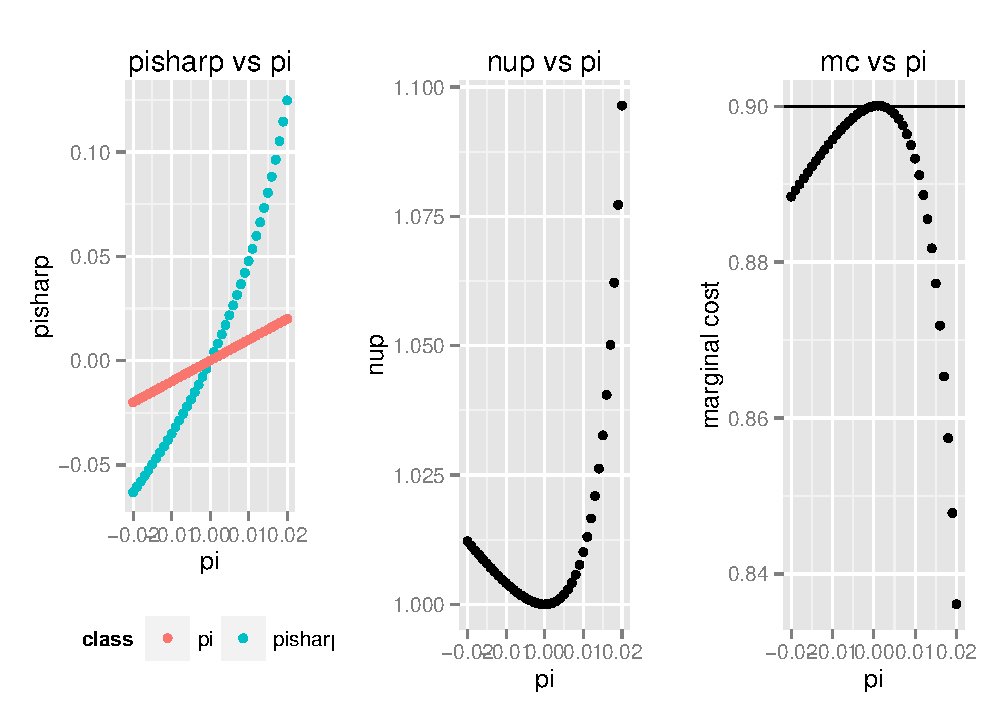
\includegraphics[width=0.8\textwidth]{Figures/R-simul-pi-pisharp-nup.pdf}
  \caption{数值模拟:$\{\pi^{\#},\nu^p\}$ vs $\pi$。模拟过程中设参数值$\phi=0.25$,$\epsilon=10$, $\beta = 0.99$。}
  \label{fig:simul-pi-pisharp-nup}
\end{figure}

给定$A=1$,工资决定式\eqref{eq:intm-prod-min-N-mc} $\Rightarrow$
\begin{equation}
  \label{eq:ss-wage}
  w = mc
\end{equation}
即工资等于劳动投入的边际成本。

式\eqref{eq:equili-agg-j-prod-DS} $\Rightarrow$ 边际产出$mpn$
\begin{equation}
  \label{eq:ss-mpn}
  mpn = \frac{1}{\nu^p}
\end{equation}
可见$\pi=0$时,mpn和mc的差距最小,体现为一个fixed price markup $\frac{\epsilon}{\epsilon -1}$。$\pi \neq 0$且越远离0时,经济体distorted的程度越大;此外,$\pi>0$时经济体的distorted程度,高于$\pi<0$时。

劳动力的供应式\eqref{HH-FOC-labor-supply} $\Rightarrow$
\begin{align*}
  \psi \cdot N^{\eta} &= C^{-\sigma} \cdot w \\
                      &= Y^{-\sigma} \cdot mc \\
                      &= \left(\frac{N}{\nu^p}\right)^{-\sigma} \cdot mc,
\end{align*}
整理得
\begin{equation}
  \label{eq:ss-labor-supply}
  N = \left[ \frac{1}{\psi} \cdot \left( \nu^p \right)^{\sigma} \cdot mc \right] ^{\frac{1}{\eta + \sigma}}
\end{equation}

总产出由式\eqref{eq:equili-agg-j-prod-DS}   \eqref{eq:ss-labor-supply}   \eqref{eq:ss-marginal-cost}得 $\Rightarrow$
\begin{align}
  \label{eq:ss-agg-output}
  Y &= \frac{N}{\nu^p},\nonumber \\
      &= \frac{\left[ \frac{1}{\psi} \cdot \left( \nu^p \right)^{\sigma} \cdot mc \right] ^{\frac{1}{\eta + \sigma}}}{\nu^p} \nonumber \\
      &= \left(\frac{1}{\psi}\right)^{\frac{1}{\sigma + \eta}} \cdot \left( v^p \right)^{-\frac{\eta}{\eta + \sigma}} \cdot
        \left[
        \frac{1-\phi \cdot \beta \cdot (1+\pi)^{\epsilon}}{1-\phi \cdot \beta \cdot (1+\pi)^{\epsilon-1}} \cdot \frac{1+\pi^{\#}}{1+\pi} \cdot \frac{\epsilon -1}{\epsilon}
        \right]^{\frac{1}{\eta + \sigma}}
\end{align}

\section{flexible price equilibrium 和 output gap}
\label{sec:flexible-price-output-gap}
\subsection{flexible price equilibrium}
\label{sec:flexible-price}

假定中间产品生产者可以自由调整价格,对应$\phi = 0$。将变量加上角标$f$以标注。此时$\pi = \pi^{\#}$,且名义价格不会对实际变量产生任何影响。

Flexible price dispersion index式\eqref{eq:price-dispersion-index-noj} $\Rightarrow$
\begin{equation}
  \label{eq:flexible-price-dispersion-index}
  v_t^{p,f} = 1,
\end{equation}
即包括最终产品和中间产品在内的全部生产者都会采取同样的产品定价策略,使price dispersion位于最低值1。

Reset price inflation 式\eqref{eq:intm-update-inflation-aux} $\Rightarrow$
\begin{equation}
  \label{eq:flexible-price-marg-cost}
  mc_t^f = \frac{\epsilon - 1}{\epsilon},
\end{equation}
可见边际成本是price markup的倒数。企业的定价策略在于:给$mc$加上一个固定的fixed price markup权数,作为产品售价。

Flexible price wage $\Rightarrow$
\begin{align*}
  mpn_t^f &= \frac{\partial Y_t^f}{\partial N_t^f} = A_t, \\
  P_t^f &= mc_t^f \cdot \frac{\epsilon}{\epsilon-1},\\
  mc_t^f &= w_t,\\
  mpn_t &= p_t^f,
\end{align*}
整理得
\begin{equation}
  \label{eq:flexible-price-wage}
  w_t^f = A_t \cdot \frac{\epsilon-1}{\epsilon}.
\end{equation}

Flexible price labor supply $\Rightarrow$
\begin{align*}
  \psi (N_t^f)^{\eta} &= (C_t^f)^{-\sigma} \cdot w_t^f,\\
                      &=(Y_t^f)^{-\sigma} \cdot mc_t^f,\\
                      &=\left( A_t \cdot N_t^f \right)^{-\sigma} \cdot \left( \frac{\epsilon -1}{\epsilon} \cdot A_t\right),
\end{align*}
整理得
\begin{equation}
  \label{eq:flexible-price-labor-supply}
  N_t^f = \left(\frac{1}{\psi} \cdot \frac{\epsilon -1}{\epsilon} \cdot A_t^{1-\sigma}\right)^{\frac{1}{\sigma + \eta}}.
\end{equation}

Flexible price aggregate output $\Rightarrow $
\begin{equation}
  \label{eq:flexible-price-agg-output}
  Y_t^f = A_t \cdot N_t^f = \left(\frac{1}{\psi} \cdot \frac{\epsilon -1}{\epsilon}\right)^{\frac{1}{\sigma + \eta}} \cdot  A_t^{\frac{1+\eta}{\sigma + \eta}}
\end{equation}

可见flexible price $(\phi =0)$情况下,名义波动不会对真实变量产生影响。

\subsection{output gap}
\label{output-gap}
定义output gap $\ln X_t \equiv \ln Y_t - \ln Y_t^f$,表示flexible price $(\phi = 0)$情况下产出$Y_t^f$与sticky price $(\phi >0)$情况下产出$Y_t$的差。

稳定状态下,$Y^f$的值由式\eqref{eq:flexible-price-agg-output}给出;
\begin{equation*}
%\label{ss-flexible-price-agg-output}
    Y^f = \left(\frac{1}{\psi} \cdot \frac{\epsilon -1}{\epsilon}\right)^{\frac{1}{\sigma + \eta}}
\end{equation*}

由此可得稳态output gap的值:
\begin{equation}
  \label{eq:ss-output-gap}
  \frac{Y}{Y^f} =
  \left[
    \frac{1-\phi \cdot \beta \cdot (1+\pi)^{\epsilon}}{1-\phi \cdot \beta \cdot (1+\pi)^{\epsilon -1}} \cdot \frac{1+\pi^{\#}}{1+\pi}
  \right]^{\frac{1}{\eta + \sigma}} \cdot
  \left(
    \nu^p
  \right)^{- \frac{\eta}{\eta + \sigma}}
\end{equation}
output gap的性质,分两种情况来讨论:

\begin{enumerate}
\item $\pi = 0$ $\Rightarrow$ $\pi^{\#} = \pi = 0$,$\nu^p = 1$ $\Rightarrow$ $Y=Y^f$ $\Rightarrow$ $\ln X = 0$,
\item $\pi >0$ $\Rightarrow$ $\pi^{\#} > \pi$, $\nu^p >1$ $\Rightarrow$ $Y<Y^f$ $\Rightarrow$ $\ln X < 0$。
\end{enumerate}
即在sticky price $(\phi >0)$条件下,稳态的output gap(对数)为负。


\section{Taylor法则}
\label{seq:Taylor-Rule}
假定中央银行的货币政策着眼于利率而非货币供应量:通过盯紧通货膨胀和产出这两个变量,灵活制定内生的货币政策以达到既定的利率目标\footnote{膏按:外生利率政策会导致indeterminacy问题,补充一个Appendix。}。常见的内生货币政策如Taylor法则:

\begin{equation}
  \label{eq:MP-Taylor-Rule}
  (i_t-i) = \rho_i \cdot (i_{t-1}-i) + (1-\rho_i) \cdot i+ (1-\rho_i) \cdot \left[
    \theta_{\pi} \cdot (\pi_t - \pi) + \theta_{x} \cdot (\ln X_t - \ln X)
  \right] + \varepsilon_{i,t},
\end{equation}
其中$i_t$表示名义利率。$X_t$表示output gap,见第\ref{output-gap}节。去掉下角标的变量表示其稳态值。$0 \le \rho_i \le 1$表示smoothing parameter。$\theta_\pi \ge 0$,$\theta_{x} \ge 0$。外生利率冲击$E\{ \varepsilon_{i,t}\} = 0$。

不难看出式\eqref{eq:MP-Taylor-Rule}的Taylor法则是个局部调整的货币政策:如果将稳态值$i$和$\pi$视作长期目标,则中央银行根据上期名义利率(距其稳态值)的偏离程度,以及当前期目标值(距其稳态值)的偏离程度,来灵活调整当期的名义利率;当前期目标值包括通货膨胀和output gap。一旦当期名义利率的调整目标确定,中央银行即通过向市场印发货币等手段,调节市场上的货币量,来实现其名义利率的目标。

\section{完整的均衡条件}
\label{sec:full-set-equilibrium-conditions}
经济系统的均衡解包括下述12个变量$\{ C_t, N_t, w_t, mc_t, Y_t, v^p_t, i_t, \pi_t, \pi^{\#}_t, x_{1,t}, x_{2,t}, A_t \}$,以及12个等式:

跨期消费的Euler equation 式\eqref{HH-FOC-euler-consumption} $\Rightarrow$
\begin{equation*}
    C_t^{-\sigma} = \beta \cdot E_t\{ C_{t+1}^{-\sigma} \cdot (1+i_t) \cdot \frac{P_t}{P_{t+1}}\}=\beta \cdot E_t\{ C_{t+1}^{-\sigma} \cdot (1+i_t) \cdot ( 1+\pi_{t+1} )^{-1}\}.
\end{equation*}

劳动力供应式\eqref{HH-FOC-labor-supply} $\Rightarrow$
\begin{equation*}
    \psi \cdot N_t^{\eta} = C_t^{-\sigma} \cdot w_t.
\end{equation*}

工资/边际成本的决定式\eqref{eq:intm-prod-min-N-mc} $\Rightarrow$
\begin{equation*}
    mc_t = \frac{MC_t}{P_t} = \frac{W_t}{A_t \cdot P_t} = \frac{w_t}{A_t}.
\end{equation*}

总消费与总产出的关系式\eqref{eq:HH-problem-C-Y} $\Rightarrow$
\begin{equation*}
  C_t = Y_t.
\end{equation*}

总量生产函数式\eqref{eq:equili-agg-j-prod-DS} $\Rightarrow$
\begin{equation*}
  Y_t = \frac{A_t \cdot N_t}{\nu^p_t}.
\end{equation*}

Price dispersion index 式\eqref{eq:price-dispersion-index-noj} $\Rightarrow$
\begin{equation*}
  \nu^p_t = (1-\phi) \cdot (1+\pi^{\#}_t)^{-\epsilon} \cdot (1+\pi_t)^{\epsilon} + \phi \cdot (1+\pi_t)^{\epsilon} \cdot \nu^p_{t-1}.
\end{equation*}

Evolution of inflation 式\eqref{eq:agg-inflation-index} $\Rightarrow$
\begin{equation*}
    \left(1+\pi_t\right)^{1-\epsilon} = (1-\phi) \cdot \left(1+\pi^{\#}_t\right)^{1-\epsilon} + \phi.
\end{equation*}

Reset price inflation 式  \eqref{eq:intm-update-inflation-aux} $\Rightarrow$
\begin{equation*}
  (1+\pi^{\#}_t) = \frac{\epsilon}{\epsilon -1} \cdot \left( 1+\pi_t \right) \cdot \frac{x_{1,t}}{x_{2,t}}.
\end{equation*}

两个reset price inflation的辅助变量,式\eqref{auxiliary-X1}-\eqref{auxiliary-X2} $\Rightarrow$
\begin{align*}
  x_{1,t} &\equiv C_t^{-\sigma} \cdot Y_t \cdot mc_t + \beta \cdot \phi \cdot E_t \left(1+\pi_{t+1} \right)^{\epsilon} \cdot x_{1,t+1},\\
  x_{2,t} &\equiv C_t^{-\sigma} \cdot Y_t + \beta \cdot \phi \cdot E_t \left( 1+\pi_{t+1} \right)^{\epsilon -1} \cdot x_{2,t+1}.
\end{align*}

Taylor rule 式\eqref{eq:MP-Taylor-Rule} $\Rightarrow$
\begin{equation*}
  (i_t-i) = \rho_i \cdot (i_{t-1}-i) + (1-\rho_i) \cdot i+ (1-\rho_i) \cdot \left[
    \theta_{\pi} \cdot (\pi_t - \pi) + \theta_{x} \cdot (\ln X_t - \ln X)
  \right] + \varepsilon_{i,t}.
\end{equation*}

Exogenous productivity shock 式\eqref{eq:exo-prod-shock} $\Rightarrow$
\begin{equation*}
  \ln A_t = \rho_a \cdot \ln A_{t-1} + \varepsilon_{a,t} .
\end{equation*}

\section{对数线性化}
\label{sec:BNK-log-lin-system}
\subsection{对数线性化计算}
\label{sec:BNK-log-linearization}
求解上述均衡方程组,方法之一是利用Dynare等计算机软件进行计算。此外,在模型较简单的情况下,也可以围绕zero-inflation steady state $\pi=0$的点,手算对数线性化的近似。

Euler equation 式\eqref{HH-FOC-euler-consumption} + 式\eqref{eq:HH-problem-C-Y} $\Rightarrow$
\begin{equation*}
  -\sigma \cdot \ln Y_t = \ln \beta - \sigma E_t \ln Y_{t+1} + i_t - E_t \pi_{t+1},
\end{equation*}
设$\ln (1+i_t) \approx i_t$,$\ln (1+\pi_t) \approx \pi_t$。将上式中每个变量分别围绕自己的稳态值作一阶泰勒级数展开,
\begin{equation*}
  -\sigma \cdot \frac{Y_t - Y}{Y} = -\sigma \cdot E_t \frac{Y_{t+1} - Y}{Y} + (i_t - i) - E_t (\pi_{t+1} - \pi),
\end{equation*}
定义$\tilde{Z}_t \equiv (Z_t - Z)/Z$作为变量$Z_t$距离其稳态值$Z$的偏离程度,$Z_t=(Y_t,N_t,A_t,\ldots)$;为了手算方便,对于已经是rate form的变量,包括利率$i_t$、通货膨胀率$\pi_t$和$\pi^{\#}_t$、price dispersion index $v^p_{t}$,直接用差分代替增速形式,如$\tilde{i}_t \equiv i_t -i$。上式进一步改写为
\begin{equation}
  \label{eq:log-lin-euler}
  \tilde{Y}_t = E_t \tilde{Y}_{t+1} - \frac{1}{\sigma} \left[\tilde{i}_t - E_t \tilde{\pi}_{t+1}\right].
\end{equation}

式\eqref{eq:log-lin-euler}又被称为New Keynesian IS Curve (NKIS)。Keynesian IS curve反映了投资(Investment)和投资(Saving)之间的对应关系。这里的“基础”New Keynesian模型中并未考虑投资,它反映了当期消费需求和实际之间的负相关关系。与传统IS curve相比,NKIS的“新”体现在其forward-looking的特征上:当期需求$(\tilde{C}_t = \tilde{Y}_t)$不只取决于实际利率$(\tilde{i}_t - E_t \tilde{\pi}_{t+1})$且负相关,还取决于对未来收入(消费)的期望$E_{t} \tilde {Y}_{t+1}$且负相关。

边际成本与工资的关系式\eqref{eq:intm-prod-min-N-mc} $\Rightarrow$
\begin{align}
  \tilde{mc}_t = \tilde{w}_t - \tilde{A}_t.
\end{align}

Price dispersion index 式\eqref{eq:price-dispersion-index-noj} $\Rightarrow$
\begin{align}
\label{eq:log-lin-price-dispersion-index}
  \tilde{\nu}^p_t &= \left[(-\epsilon) \cdot (1-\phi) \cdot (1+\pi^{\#})^{-\epsilon -1} \cdot (1+\pi)^{\epsilon}\right] \cdot (\pi^{\#}_t - \pi^{\#}) \nonumber\\
                    &+ \left[ \epsilon \cdot (1-\phi) \cdot (1+\pi^{\#})^{-\epsilon} \cdot (1+\pi)^{\epsilon -1} \right] \cdot \pi_t \nonumber\\
                    &+\left[ \epsilon \cdot \phi \cdot (1+\pi)^{\epsilon -1} \cdot \nu^p \right] \cdot (\pi_t - \pi) \nonumber\\
                    &+\left[ \phi \cdot (1+\pi)^{\epsilon} \right] \cdot \left(\nu^p_{t-1} - \nu^p \right) \nonumber\\
                  &=-\epsilon \cdot (1-\phi) \cdot \tilde{\pi}^{\#}_t + \epsilon \cdot (1-\phi) \cdot \tilde{\pi}_t + \epsilon \cdot \phi \cdot \tilde{\pi}_t + \phi \cdot \tilde{\nu}^p_{t-1} \nonumber\\
                    &=-\epsilon \cdot (1-\phi) \cdot \tilde{\pi}^{\#}_t + \epsilon \cdot \tilde{\pi}_t + \phi \cdot \tilde{\nu}^p_{t-1},
\end{align}
其中第三个等号用到$\pi = \pi^{\#} = 0$的假设条件。


Evolution of inflation 式\eqref{eq:agg-inflation-index} $\Rightarrow$
\begin{equation*}
  (1-\epsilon) \cdot \ln (1+\pi_t) = \ln \left[ (1-\phi) \cdot \left(1+\pi^{\#}_t\right)^{1-\epsilon} + \phi \right],
\end{equation*}
\begin{equation*}
  (1-\epsilon) \cdot (\pi_t - \pi) =
  \left[
    (1-\phi) \cdot (1-\epsilon) \cdot \left( 1+\phi^{\#} \right)^{-\epsilon} \cdot (1+\pi)^{\epsilon -1}
  \right],
\end{equation*}
\begin{equation}
  \label{log-lin-evolution-inflation}
  \tilde{\pi}_t = (1-\phi) \cdot \tilde{\pi}^{\#}_t.
\end{equation}

由式\eqref{log-lin-evolution-inflation}可见,actual inflation和reset price inflation呈一定比例变化,比例$1-\phi$为全部企业中,调整价格者所占的比重。

总量生产函数式\eqref{eq:equili-agg-j-prod-DS} $\Rightarrow$
\begin{align}
  \label{eq:log-lin-agg-prod-func}
  \tilde{Y}_t &= \tilde{A}_t + \tilde{N}_t - \tilde{\nu}^p_t \nonumber \\
              &=\tilde{A}_t + \tilde{N}_t - \left[\epsilon \cdot \tilde{\pi}_t -\epsilon \cdot (1-\phi) \cdot \tilde{\pi}^{\#}_t + \phi \cdot \tilde{\nu}^p_{t-1}\right]\nonumber \\
              &\approx \tilde{A}_t + \tilde{N}_t,
\end{align}
第三行的约等号是由于,从式\eqref{eq:log-lin-price-dispersion-index}可得,在zero inflation steady state下,$\pi=\pi^{\#}=0$且$\nu^p=1$,则$(\nu^p_t-1) = \phi \cdot (\nu^p_{t-1}-1)$。这说明$\tilde{\nu}^p_t=0$ $\forall t$。换句话说,在price dispersion index是一个二阶量;在我们围绕zero inflation steady state作一阶线性近似时,可以省略。

flexible price下的产出水平式\eqref{eq:flexible-price-agg-output} $\Rightarrow$
\begin{equation}
  \label{eq:log-lin-flexible-price-output}
  \tilde{Y}_t^f = \frac{1+\eta}{\sigma + \eta} \cdot \tilde{A}_t.
\end{equation}

劳动力供应式\eqref{HH-FOC-labor-supply} $\Rightarrow$
\begin{align*}
%\label{log-lin-labor-supply}
    \eta \cdot \tilde{N}_t &= -\sigma \cdot \tilde{Y}_t + \tilde{w}_t \nonumber \\
                           &= -\sigma \cdot \tilde{Y}_t + \tilde{mc}_t + \tilde{A}_t,
\end{align*}
引入式\eqref{eq:log-lin-agg-prod-func}替代LHS的$\tilde{N}_t$,引入式\eqref{eq:flexible-price-agg-output}替代RHS的$\tilde{A}_t$,可得
\begin{align}
  \label{eq:log-lin-labor-supply}
  \tilde{mc}_t &= \left(\sigma + \eta \right) \cdot \tilde{Y}_t - (1+\eta) \cdot \tilde{A}_t \nonumber \\
               &= (\sigma + \eta) \cdot \tilde{Y}_t - \left(\frac{\sigma + \eta}{1+\eta} \right) \cdot \tilde{Y}^f_t \cdot (1+\eta)\nonumber \\
               &= (\sigma + \eta) \cdot \left(\tilde{Y}_t - \tilde{Y}^f_t \right) \nonumber \\
               &= (\sigma + \eta) \cdot \tilde{X}_t,
\end{align}
式\eqref{eq:log-lin-labor-supply} LHS是fixed steady state price markup的倒数$(\epsilon - 1 )/\epsilon$。
\begin{enumerate}
\item $\tilde{X}_t = 0$ $\Rightarrow$ $\tilde{mc}_t = 0$ $\Rightarrow$ $mc_t \equiv mc = \frac{\epsilon-1}{\epsilon}$ $\Rightarrow$ price markups等于desired steady state fixed price markup $\frac{\epsilon}{\epsilon -1}$
\item $\tilde{X}_t <0$ $\Rightarrow$ $Y_t < Y_t^f$ $\Rightarrow$ $\tilde{mc}_t < mc$ $\Rightarrow$ 实际边际成本小于steady state fixed price markup, $mc_t < \frac{\epsilon}{\epsilon -1}$ $\Rightarrow$ 该经济体 is more distorted。
\end{enumerate}

辅助变量$x_{1,t}$式\eqref{auxiliary-X1} $\Rightarrow$
\begin{equation*}
  \ln x_{1,t} = \ln \left[ Y_t^{1-\sigma} \cdot mc_t + \phi \cdot \beta \cdot E_t \cdot (1+\pi_{t+1})^{\epsilon} \cdot x_{1,t+1}\right],
\end{equation*}
\begin{align}
\label{log-lin-X1-step1}
  \frac{x_{1,t} - x_{1}}{x_1} &= \frac{1}{x_1} \cdot \{ \left[(1-\sigma) \cdot Y^{-\sigma} \cdot mc \right]\cdot (Y_t - Y) \nonumber\\
                              &+Y^{1-\sigma} \cdot (mc_t - mc) \nonumber\\
                              &+\left[\phi \cdot \beta \cdot \epsilon \cdot (1+\pi)^{\epsilon -1} \cdot x_1\right] \cdot E_t (\pi_{t+1}-\pi)\nonumber\\
                              &+\left[ \phi \cdot \beta \cdot (1+\pi)^{\epsilon}\right] \cdot E_t (x_{1,t+1} - x_1) \},
\end{align}
由式\eqref{auxiliary-X1}可得,在$\pi = 0$时
\begin{equation}
\label{log-lin-X1-step2}
  x_{1} = \frac{Y^{-\sigma} \cdot mc}{1-\phi \cdot \beta},
\end{equation}
联立\eqref{log-lin-X1-step1}-\eqref{log-lin-X1-step2}得
\begin{equation}
\label{log-lin-X1-step3}
  \tilde{x}_{1,t} = (1-\sigma) \cdot (1-\phi \cdot \beta) \cdot \tilde{Y}_t + (1-\phi \cdot \beta) \cdot \tilde{mc}_t + \epsilon \cdot \phi \cdot \beta \cdot E_t \tilde{\pi}_{t+1} + \phi \cdot \beta \cdot E_t \tilde{x}_{1,t+1}.
\end{equation}

辅助变量$x_{2,t}$式\eqref{auxiliary-X2} $\Rightarrow$
\begin{equation*}
  \ln x_{2,t} = \ln \left[Y_t^{1-\sigma} + \phi \cdot \beta \cdot E_t \left(1+\pi_{t+1}\right)^{\epsilon -1} \cdot x_{2,t+1}\right],
\end{equation*}
\begin{align}
\label{eq:log-lin-X2-step1}
  \frac{x_{2,t}-x_2}{x_2} &= \frac{1}{x_2} \cdot \{ \left[(1-\sigma) \cdot Y^{-\sigma}\right] \cdot (Y_t - Y)\nonumber\\
                          &+\left[\phi \cdot \beta \cdot E_t (\epsilon -1) \cdot (1+\pi)^{\epsilon -2} \cdot x_2\right] \cdot (\pi_{t+1} - \pi)\nonumber\\
                          &+\left[\phi \cdot \beta \cdot E_t (1+\pi)^{\epsilon -1} \right] \cdot \left( x_{2,t+1} - x_2\right),
\end{align}
由式\eqref{auxiliary-X2}可得,在$\pi = 0$时
\begin{equation}
  \label{eq:log-lin-X2-step2}
  x_2 = \frac{Y^{-\sigma}}{1-\phi \cdot \beta}
\end{equation}

联立式\eqref{eq:log-lin-X2-step1}-\eqref{eq:log-lin-X2-step2}得
\begin{equation}
  \label{eq:log-lin-X2-step3}
  \tilde{x}_{2,t} = (1-\sigma) \cdot (1-\phi \cdot \beta) \cdot \tilde{Y}_t+ (\epsilon - 1) \cdot \phi \cdot \beta \cdot E_t \tilde{\pi}_{t+1} + \phi \cdot \beta \cdot E_t \tilde{x}_{2,t+1}.
\end{equation}

将式\eqref{eq:log-lin-X2-step3}-\eqref{eq:log-lin-X2-step3}代入式\eqref{eq:intm-update-inflation-aux}得
\begin{align}
\label{log-lin-reset-price-inflation-step1}
  \tilde{\pi}^{\#}_t - \tilde{\pi}_t &= \tilde{x}_{1,t}-\tilde{x}_{2,t} \nonumber \\
                     &=(1-\phi \cdot \beta) \cdot \tilde{mc}_t + \phi \cdot \beta \cdot E_t \tilde{\pi}_{t+1} + \phi \cdot \beta \cdot E_t \left(\tilde{x}_{1,t+1} - \tilde{x}_{2,t+1} \right).
\end{align}

式\eqref{log-lin-evolution-inflation}与\eqref{log-lin-reset-price-inflation-step1}联立,可得 Reset price inflation式
\begin{equation}
  \label{eq:log-lin-reset-price-inflation-mc}
  \tilde{\pi}_t = \left(\frac{1-\phi}{\phi}\right) \cdot (1-\phi \cdot \beta) \cdot \tilde{mc}_{t} + \beta \cdot E_t \tilde{\pi}_{t+1}.
\end{equation}

式\eqref{eq:log-lin-reset-price-inflation-mc}又被称为New Keynesian Philips Curve (NKPC),它反映了中央银行对产出和通货膨胀的trade off。也可以用式\eqref{eq:log-lin-labor-supply}中的output gap $\tilde{X}_t$代替边际成本$mc_{t}$,NKPC改写为
\begin{align}
  \label{eq:log-lin-reset-price-inflation-gap}
  \tilde{\pi}_t &= \left(\frac{1-\phi}{\phi}\right) \cdot (1-\phi \cdot \beta) \cdot \left[(\sigma + \eta) \cdot \left(\tilde{Y}_t - \tilde{Y}_t^f \right)\right] + \beta \cdot E_t \tilde{\pi}_{t+1}\nonumber \\
                &= \left(\frac{1-\phi}{\phi}\right) \cdot (1-\phi \cdot \beta) \cdot \left[(\sigma + \eta) \cdot \tilde{X}_t \right] + \beta \cdot E_t \tilde{\pi}_{t+1}.
\end{align}

或者,around a zero inflation steady state,用forward-looking形式表现NKPC
\begin{align}
  \label{eq:log-lin-reset-price-inflation-4ward-mc}
  \tilde{\pi_t} &= \left(\frac{1-\phi}{\phi}\right) \cdot (1-\phi \cdot \beta) \cdot \sum_{s=0}^{\infty} \beta^s \cdot \tilde{mc}_{t+s} \\
  \label{eq:log-lin-reset-price-inflation-4ward-gap}
                &= \left(\frac{1-\phi}{\phi}\right) \cdot (1-\phi \cdot \beta) \cdot (\sigma +\eta) \cdot \sum_{s=0}^{\infty} \beta^s \cdot \tilde{X}_{t+s}.
\end{align}

Keynesian PC curve 反映了通货膨胀率和边际成本之间的对应关系。NKPC的“新”体现在其forward-looking的特征上。  式\eqref{eq:log-lin-reset-price-inflation-4ward-mc}表明当前通货膨胀率和对未来实际边际成本的贴现值之间呈等比关系,边际成本表现为price markup的倒数。在价格是完全浮动的情况下$\phi = 0$,企业会根据desired constant markups给产品定价;如果企业预期未来的边际成本会增加,那么在定价时就会相应调低price markups。在存在价格粘性的情况下$\phi >0$,有机会在当前$t$期调整价格的企业,便会提前提高产品价格(以避免在未来$t+s$时间期内无法再次调整产品售价),以达到他们的desired price markup,这造成了通货膨胀。反之亦然。

NKPC curve的“斜率”与$\phi$负相关。随着$\phi$逐渐降低,NKPC线越来越陡峭。当$\phi \rightarrow 0$时,perfectly flexible price,NKPC线完全垂直,此时$\tilde{Y}_t = \tilde{Y}_t^f$,$\tilde{mc}_t = 0$。

Exogenous productivity shock 式\eqref{eq:exo-prod-shock} $\Rightarrow$
\begin{equation}
  \label{eq:log-lin-prod-shock}
  \tilde{A}_t =\rho_a \cdot \tilde{A}_{t-1} + \varepsilon_{a,t}.
\end{equation}

Taylor rule 式\eqref{eq:MP-Taylor-Rule} $\Rightarrow$
\begin{equation}
  \label{eq:log-lin-tayl-rule}
  \tilde{i}_t = \rho_i \cdot \tilde{i}_{t-1} + (1-\rho_i) \cdot \left[\phi_{\pi} \cdot \tilde{\pi}_t + \phi_{x} \cdot \tilde{X}_t \right].
\end{equation}

\subsection{线性模型}
\label{sec:BNK-log-linearization-system}
作线性近似处理后的经济系统,表述为如下5个变量$\left(\tilde{Y}_t, \tilde{i}_t, \tilde{\pi}_t, \tilde{Y}_t^f, \tilde{A}_t\right)$,5个等式
线性Euler equation,反映总量需求的NKIS式\eqref{eq:log-lin-euler} $\Rightarrow$
\begin{equation*}
  \tilde{Y}_t = E_t \tilde{Y}_{t+1} - \frac{1}{\sigma} \left(\tilde{i}_t - E_t \tilde{\pi}_{t+1}\right).
\end{equation*}

反映总量供应的NKPC式\eqref{eq:log-lin-reset-price-inflation-mc}或  \eqref{eq:log-lin-reset-price-inflation-gap} $\Rightarrow$
\begin{align*}
  \tilde{\pi}_t &= \left(\frac{1-\phi}{\phi}\right) \cdot (1-\phi \cdot \beta) \cdot \tilde{mc}_{t} + \beta \cdot E_t \tilde{\pi}_{t+1}\\
                &=\left(\frac{1-\phi}{\phi}\right) \cdot (1-\phi \cdot \beta) \cdot \left[(\sigma + \eta) \cdot \tilde{X}_t \right] + \beta \cdot E_t \tilde{\pi}_{t+1}.
\end{align*}

辅助变量,反映flexible price下的产出水平,式\eqref{eq:log-lin-flexible-price-output} $\Rightarrow$
\begin{equation*}
  \tilde{Y}_t^f = \frac{1+\eta}{\sigma + \eta} \cdot \tilde{A}_t.
\end{equation*}

Exogenous productivity shock 式\eqref{eq:exo-prod-shock} $\Rightarrow$
\begin{equation*}
  \tilde{A}_t =\rho_a \cdot \tilde{A}_{t-1} + \varepsilon_{a,t}.
\end{equation*}

反映货币政策的Taylor rule 式\eqref{eq:MP-Taylor-Rule} $\Rightarrow$
\begin{equation*}
  \tilde{i}_t = \rho_i \cdot \tilde{i}_{t-1} + (1-\rho_i) \cdot \left[\phi_{\pi} \cdot \tilde{\pi}_t + \phi_{x} \cdot \tilde{X}_t \right].
\end{equation*}

%!TEX root = ../DSGEnotes.tex
\chapter{Medium-Sized DSGE模型}
\section{产品的生产部门}
\label{sec:production-sector}


\subsection{最终产品生产部门}
\label{sec:final-production-sector}
最终产品生产部门以中间产品$Y_t(i), i \in (0,1)$的组合为投入要素,产出$Y_t$,符合完全竞争假定。\cite{Dixit:1977tv}形式的生产规模报酬不变生产函数为
\begin{equation}
  \label{eq:fin-prod-prod-func-me}
  Y_t = \left[ \int_{0}^{1} Y_t(i)^{\frac{\varepsilon_{f} - 1}{\varepsilon_{f}}} \, di \right]^{\frac{\varepsilon_{f}}{\varepsilon_{f} - 1}},
\end{equation}
其中$\varepsilon_f$表示$i^{th}$中间产品的替代弹性。

最终产品厂商问题:在给定中间产品价格$P_t(i)$的情况下,通过选择$Y_t(i)$的投入追求利润最大化

\begin{equation*}
%  \label{eq:fin-prod-problem-max}
  \max_{Y_t(i)} P_t \cdot Y_t - \int_{0}^{1} P_t(i) \cdot Y_t(i) di.
\end{equation*}

引入式\eqref{eq:fin-prod-prod-func},FOC整理可得对$i$中间产品的需求函数
\begin{equation}
  \label{eq:demand-for-intm-i}
  Y_t(i) = \left( \frac{P_t(i)}{P_t}
\right)^{-\varepsilon_f} \cdot Y_t,
\end{equation}

进而根据完全竞争市场假定
\begin{equation*}
  \begin{split}
    P_t \cdot Y_t & \equiv \int_0^1 P_t(i) \cdot Y_t(i) di \\
    &=\left[\int_0^1 \left(\frac{P_t(i)}{P_t}\right)^{-\varepsilon_f} \cdot Y_t \cdot P_t(i) di \right] \\
    &=\left[\int_0^1 P_t(i)^{1-\varepsilon_f} di \right] \cdot P_t^{\varepsilon_f} \cdot Y_t,\\
  \end{split}
\end{equation*}
整理得最终产品价格的决定(aggregate price index):
\begin{equation}
  \label{eq:agg-price-index-me}
  P_t = \left[
    \int_0^1 P_t(i)^{1-\varepsilon_f} di
  \right]^{\frac{1}{1-\varepsilon_f}}
\end{equation}


\subsection{中间产品生产部门}
\label{sec:intm-production-sector}
每个$i^{th}$中间产品有且只有一个生产者,处于垄断竞争状态,视式\eqref{eq:demand-for-intm-i}-\eqref{eq:agg-price-index}为需求函数和价格;最终产品的总产出$Y_t$和总价格$P_t$是外生的。$i^{th}$中间品生产者的生产函数为
\begin{equation}
  \label{eq:intm-prodc-func-me}
  Y_t(i) = K_t(i)^{\alpha} \cdot \left[ z_t \cdot H_{t}(i) \right]^{1-\alpha}  - z_t^+ \cdot \varphi,
\end{equation}
其中投入要素$H_t(i)$和$K_{t}(i)$分别表示同质的劳动力和实物资本服务,产出系数$0<\alpha<1$。$z_t$和$\Psi_t$分别表示neutral和investment-specific类型的随机技术冲击,见第\ref{sec:total-output-allocation}节。$\varphi$为生产的固定成本;$z_t^+$定义如下
\begin{equation}
  \label{eq:ztplus-zt-Psi}
  z_t^+ = \Psi_t^{\frac{\alpha}{1-\alpha}} \cdot z_t,
\end{equation}
可见沿着非随机的稳态增长路径,$Y_{t}(i)/z_t^+$收敛至常数\footnote{膏按:模型引入固定成本的设定,以及采取一个变量乘以一个常量形式设定的考虑。模型假定中间产品生产者处于垄断地位,且假定没有进出(no entry and exit),以确保垄断利润得以长期持续,因此在中间产品生产函数中引入常数固定生产成本$\varphi$,使得稳态利润是零,被固定成本抵消,维持no entry的假设成立。但这需要fixed cost的增速与产出增速相等,由此对常数$\varphi$额外乘以一个系数$z_t^+$。此外经验研究的发现也肯定了这种设定的意义:在引入规模报酬递增的情况下,正的货币政策冲击产生后,劳动的生产率随着提高,这与对现实的观测基本接近。}。

$i^{th}$中间产品生产者雇佣同质劳动服务$H_{t}(i)$,假定生产者必须100\%借款来支付工资,根据\cite{Christiano:2005ib}的working capital channel设定加以简化$(v_t = 0, \psi = 1)$,每一单位劳动服务的成本等于
\begin{equation*}
  cost = (1-v_t) \cdot (1-\psi + \psi \cdot R_t) \cdot W_t = R_t \cdot W_t,
\end{equation*}
其中$W_t$和$R_t$分别表示总量水平上的名义工资和working capital借贷的名义利率\footnote{Working Capital Channel可追溯至\cite{Basu:1995vl}。\cite{Christiano:2005ib}对资本和劳动服务的working capital做了建模。近期研究可见\cite{Phaneuf:2015vp}。根据不含working capital channel的DSGE模型模拟出来的结果,对经济体注入正的货币政策冲击会导致通货膨胀率有大幅度的提升,而现实世界中通货膨胀并没有上升的如此剧烈。\cite{Christiano:2005ib}因此引入了working capital channel设定以缓解该问题,其思路如下:正的货币政策冲击降低了名义利率,进而降低企业进行外部融资(支付员工工资)的边际成本,而边际成本对企业价格决策的制定至关重要。一系列对经济现实的VAR-based观察发现,扩张性货币政策冲击出现后的初期,通货膨胀率出现小幅的下降。这从侧面印证了working capiutal channel假设的重要性,除了可能存在计量意义上的设定失误之外,恐怕只有working capital channel的假设可以解释它了。计量意义上的设定失误,\cite{Sims:1992bw}最早提出这种可能;\cite{Christiano:1999uw}进一步探讨了该可能性;另外可见\cite{Bernanke:2005vn}。}。



经济体受到的外部技术冲击有二,分别为$z_t$和$\Psi_t$,均假定为对数形式的单位根过程\footnote{膏按:式\eqref{eq:tech-shock-zt}直接将中性技术进步定义为有drift的随机游走过程,依据如下:
  \begin{enumerate}
  \item estimation部分,\cite{Smets:2003ik}估计$\log z_t$发现它高度自相关,
  \item \cite{Prescott:1986ej}的经验研究 ,
  \item \cite{Fernald2009}对美国经济部门的经验研究发现,1947年第2季度到2009年第三季度TFP增速的一阶自回归系数为0.0034。
  \end{enumerate}
}:
\begin{equation}
  \label{eq:tech-shock-zt}
  \Delta \log z_t = \mu_z + \varepsilon_{z,t}, E(\varepsilon_{z,t}) = \sigma^2_{z},
\end{equation}
\begin{equation}
  \label{eq:tech-shock-Psi}
  \Delta \log \Psi_t = (1-\rho_{\Psi}) \cdot \mu_{\Psi} + \rho_{\Psi} \cdot \Delta \log \Psi_{t-1} + \varepsilon_{\Psi, t}, E(\varepsilon_{\Psi,t}) = \sigma^2_{\Psi}.
\end{equation}


\subsection{中间产品生产者的边际成本}
\label{seq:marg-cost-intm-producer}
$i^{th}$中间产品生产者的最优行为表现为两阶段优化。第一阶段是成本最小化,选择合适的投入要素$\{K_{t}(i), H_{t}(i)\}$数量,生产出满足最终产品生产部门需求的$Y_t(i)$。投入要素价格分别为市场给定的$\bar{R_t}$及$\bar{W}_t$,
\begin{align*}
  \min_{K_{t}(i), H_{t}(i)} &\bar{W}_t \cdot H_t(i) + \bar{R}_t \cdot K_{t}(i), \\
  & st. \quad  Y_t(i) = K_t(i)^{\alpha} \cdot \left[ z_t \cdot H_{t}(i) \right]^{1-\alpha}  -  z_t^+ \cdot \varphi.
\end{align*}

建Lagrangian
\begin{equation*}
  \mathcal{L} = \bar{W}_t \cdot H_t(i) + \bar{R}_t \cdot K_{t}(i) +\lambda_t \cdot \left\{Y_t(i) - K_t(i)^{\alpha} \cdot \left[ z_t \cdot H_{t}(i) \right]^{1-\alpha}  +  z_t^+ \cdot \varphi \right\}.
\end{equation*}

FOCs:
\begin{align}
  \label{eq:intm-marg-min-cost-FOC-H}
  \frac{\partial \mathcal{L}}{\partial H_{t}(i)} = 0 &\Rightarrow \bar{W}_t = \lambda_t \cdot (1-\alpha) \cdot z_t^{1-\alpha} \cdot H_{t}(i)^{-\alpha} \cdot K_{t}(i)^{\alpha},\\
  \label{eq:intm-marg-min-cost-FOC-K}
\frac{\partial \mathcal{L}}{\partial K_{t}(i)} = 0 &\Rightarrow \bar{R}_t = \lambda_t \cdot \alpha \cdot z_t^{1-\alpha} \cdot H_{t}(i)^{1-\alpha} \cdot K_{t}(i)^{\alpha-1}.
\end{align}

式\eqref{eq:intm-marg-min-cost-FOC-H}-  \eqref{eq:intm-marg-min-cost-FOC-K}可得
\begin{equation}
  \label{eq:intm-marg-min-cost-FOC-W-R}
  \frac{\bar{W}_t}{\bar{R}_t} = \left(\frac{\alpha}{1-\alpha}\right)^{-1} \cdot \left(\frac{K_{t}(i)}{H_{t}(i)}\right).
\end{equation}

由式\eqref{eq:intm-marg-min-cost-FOC-W-R}可得 \begin{equation}
\label{eq:intm-homo-K-H-no-i} \frac{K_t(i)}{H_{t}(i)} \equiv \frac{K_t}{H_t},
\quad \forall i, \end{equation} 即所有中间产品生产者以及总量层面上的投入要素之比相等。

将式\eqref{eq:intm-marg-min-cost-FOC-W-R}带回生产函数式\eqref{eq:intm-prodc-func},得
\begin{equation*}
  Y_t(i) + z_t^+ \cdot \varphi
= z_t^{1-\alpha} \cdot \left(\frac{\bar{W}_t}{\bar{R}_t}\right)^{-(1-\alpha)} \cdot \left( \frac{\alpha}{1-\alpha} \right)^{-(1-\alpha)} \cdot K_{t}(i)
= z_t^{1-\alpha} \cdot \left(\frac{\bar{W}_t}{\bar{R}_t}\right)^{\alpha} \cdot \left( \frac{\alpha}{1-\alpha} \right)^{\alpha} \cdot H_{t}(i).
\end{equation*}

进而最优投入要素的数量
\begin{align*}
%  \label{eq:intm-marg-min-cost-K}
  K_t(i) &= \left[ Y_t(i) + z_t^+ \cdot \varphi \right] \cdot z_t^{-(1-\alpha)} \cdot \left(\frac{\bar{W}_t}{\bar{R}_t}\right)^{1-\alpha} \cdot \left( \frac{\alpha}{1-\alpha} \right)^{1-\alpha}, \\
%  \label{eq:intm-marg-min-cost-H}
  H_t(i) &= \left[ Y_t(i) + z_t^+ \cdot \varphi \right] \cdot z_t^{-(1-\alpha)} \cdot \left(\frac{\bar{W}_t}{\bar{R}_t}\right)^{-\alpha} \cdot \left( \frac{\alpha}{1-\alpha} \right)^{-\alpha}.
\end{align*}

$i^{th}$中间产品生产者的成本函数
\begin{equation}
  \label{eq:intm-prodc-cost}
  C(Y_t(i),K_t(i),H_t(i)) =\bar{W}_t \cdot H_t(i) + \bar{R}_t \cdot K_{t}(i) = \left(Y_t(i) + z_t^+ \cdot \varphi \right) \cdot z_t^{-(1-\alpha)} \cdot \left(\frac{\bar{W}_t}{1-\alpha}\right)^{1-\alpha} \cdot \left(\frac{\bar{R}_t}{\alpha}\right)^{\alpha}.
\end{equation}

因此名义边际成本$S_t(i)$等于
\begin{equation}
  \label{eq:intm-nominal-marg-cost}
  S_t(i) = \frac{\partial C(Y_t(i),K_t(i),H_t(i))}{\partial Y_t(i)} = z_t^{-(1-\alpha)} \cdot \left(\frac{\bar{W}_t}{1-\alpha}\right)^{1-\alpha} \cdot \left(\frac{\bar{R}_t}{\alpha}\right)^{\alpha},
\end{equation}
类似地,$S_t(i) \equiv S_t, \forall i$。

根据定义,投入要素的市场价格
\begin{align}
  \label{intm-mkt-price-real-price-W}
  \bar{W}_t &= (1-v_t) \cdot (1-\psi + \psi \cdot R_t) \cdot W_t,\\
  \label{intm-mkt-price-real-price-R}
  \bar{R}_t &= (1-v_t) \cdot (1-\psi + \psi \cdot r_t^k) \cdot P_t
\end{align}

引入$v_t=0,\psi = 1$的设定后,实际边际成本$s_t$等于
\begin{align}
  \label{intm-mkt-real-mrg-cost}
s_t \equiv \frac{S_t}{P_t} = \frac{\left(\frac{R_t \cdot W_t}{1-\alpha}\right)^{1-\alpha} \cdot \left(\frac{r_t^k \cdot P_t}{\alpha}\right)^{\alpha}}{z_t^{1-\alpha} \cdot P_t}.
\end{align}

引入式  \eqref{eq:real-rental-rate-capital}、  \eqref{eq:scaled-real-wage}、\eqref{eq:ztplus-zt-Psi}后,式\eqref{intm-mkt-real-mrg-cost}改写为scaled形式
\begin{equation}
  \label{eq:intm-mkt-real-mrg-cost-scaled}
  s_t = \frac{\left(\frac{R_t \cdot \left(\bar{w}_t \cdot z_t^+ \cdot P_t \right)}{1-\alpha}\right)^{1-\alpha} \cdot \left(\frac{\left(\frac{\bar{r}_t^k}{\Psi_t}\right) \cdot P_t}{\alpha}\right)^{\alpha}}{z_t^{1-\alpha} \cdot P_t} = \left( \frac{\bar{w}_t \cdot R_t} {1-\alpha}\right)^{1-\alpha} \cdot \left( \frac{\bar{r}_{t}^k}{\alpha}\right)^{\alpha}.
\end{equation}

此外,根据productive efficiency,生产额外1单位$Y_t(i)$的边际成本$s_t$,等于雇佣额外1单位劳动的成本$W_t \cdot R_t$,除以劳动的名义边际产出$P_t \cdot \frac{\partial Y_t(i)}{\partial H_{t}(i)}$,即
\begin{equation}
  \label{eq:intm-mkt-real-mrg-cost-efficiency}
\begin{split}
  s_t
  &= \frac{W_t \cdot R_t}{P_t \cdot \frac{\partial Y_t(i)}{\partial H_t(i)}} \\
  &= \frac{\left(\bar{w}_t \cdot z_t^+ \cdot P_t\right) \cdot R_t}{(1-\alpha) \cdot \left[\frac{K_t(i)}{H_{t}(i)}\right]^{\alpha} \cdot z_t^{1-\alpha} \cdot P_t} \\
  &= \frac{\bar{w}_t \cdot R_t \cdot z_t^+ \cdot P_t}{(1-\alpha) \cdot \left[\frac{\frac{k_t(i)}{z_{t-1}^+ \cdot \Psi_{t-1}}}{H_{t}(i)}\right]^{\alpha} \cdot \left(z_t^+ \cdot \Psi^{-\frac{\alpha}{1-\alpha}}\right)^{1-\alpha} \cdot P_t} \\
      &=\frac{\bar{w}_t \cdot R_t}{(1-\alpha) \cdot \left[\frac{k_{t}(i)}{H_t(i) \cdot \mu_{z^{+},t} \cdot \mu_{\Psi, t}}\right]^{\alpha}}\\
        &= \frac{\bar{w}_t \cdot R_t \cdot z_t^+ \cdot P_t}{(1-\alpha) \cdot \left[\frac{\frac{k_t(i)}{z_{t-1}^+ \cdot \Psi_{t-1}}}{H_{t}(i)}\right]^{\alpha} \cdot \left(z_t^+ \cdot \Psi^{-\frac{\alpha}{1-\alpha}}\right)^{1-\alpha} \cdot P_t} \\
      &=\frac{\bar{w}_t \cdot R_t}{(1-\alpha) \cdot \left[\frac{k_{t}}{H_t \cdot \mu_{z^{+},t} \cdot \mu_{\Psi, t}}\right]^{\alpha}}.
\end{split}
\end{equation}
其中最后一个等号利用式\eqref{eq:output-scaled}消除异质性。



\subsection{中间产品生产者的定价}
\label{sec:intm-pricing-calvo}

\subsubsection{updating生产者的定价策略}
\label{seq:intm-updating-pricing}

价格刚性。假定在$t$时期,有$0 \le \phi_f \le 1$比例的中间产品生产者$i \in [0,1]$无法调整价格;有$1-\phi_f$比例的生产者不可以调整价格。可以调整价格的中间产品垄断生产者,其forward-looking问题可以描述为,制定合理的垄断价格$P_t^{\#}(i)$以满足利润最大化
\begin{equation}
  \label{eq:intm-pricing-problem-1}
  \max_{P_{t}^{\#}(i)} E_t \sum_{j=0}^{\infty}\left( \phi_f \cdot \beta \right)^j \cdot v_{t+j} \cdot \left[P_{t}^{\#}(i) \cdot Y_{t+j}(i) - P_{t+j} \cdot s_{t+j} \cdot Y_{t+j}(i)\right],
\end{equation}
st. 对$i^{th}$中间产品的需求式\eqref{eq:demand-for-intm-i}。$s_t$的定义见式  \eqref{eq:intm-mkt-real-mrg-cost-scaled}。中括号中的内容为$t+j$时刻$i^{th}$生产者的利润;$\beta^j \cdot v_{t+j}$为家庭部门跨期预算约束条件的乘数\footnote{中间产品生产部门的垄断利润,假设全部返回家庭部门;家庭部门基于自己的消费偏好作跨期消费决策;因此对于$i^{th}$来说,$\beta^j \cdot v_{t+j}$是外生给定的。},满足$v_{t}=\frac{\partial U_t(\cdot) / \partial C_t}{P_t}$。\footnote{膏按:补一个eqref,嵌到hh部门的max problem上去。}

引入式\eqref{eq:demand-for-intm-i}替代$Y_{t+j}(i)$,整理得
\begin{align*}
%  \label{eq:intm-pricing-problem-2}
  &\max_{P_{t}^{\#}(i)} E_t \sum_{j=0}^{\infty}\left( \phi_f \cdot \beta \right)^j \cdot
\left(\frac{U_{C,t+j}}{P_{t+j}}\right) \cdot
\left(
  \frac{P_{t+j}^{\#}(i)}{P_{t+j}}
\right)^{-\varepsilon_f} \cdot Y_{t+j} \cdot
\left[P_{t}^{\#}(i)  - P_{t+j} \cdot s_{t+j} \right]\\
=&\max_{P_{t}^{\#}(i)} E_t \sum_{j=0}^{\infty}\left( \phi_f \cdot \beta \right)^j \cdot
\left(
U_{C,t+j} \cdot Y_{t+j}
\right) \cdot
\left[P_{t}^{\#}(i)^{-(\varepsilon_f - 1)}  \cdot P_{t+j}^{\varepsilon_f -1}- P_{t}^{\#}(i)^{-\varepsilon_f} \cdot P_{t+j}^{\varepsilon_f} \cdot s_{t+j} \right].
\end{align*}

FOC wrt $P_{t}^{\#}(i)$,
\begin{align*}
&  \left[-(\varepsilon_f - 1)\right] \cdot
\max_{P_{t}^{\#}(i)} E_t \sum_{j=0}^{\infty}\left( \phi_f \cdot \beta \right)^j \cdot
\left(
U_{C,t+j} \cdot Y_{t+j}
\right) \cdot
\left[
  P_{t}^{\#}(i)^{-\varepsilon_f} \cdot P_{t+j}^{\varepsilon_f - 1}
\right] \\
=& -\varepsilon_f \cdot
\max_{P_{t}^{\#}(i)} E_t \sum_{j=0}^{\infty}\left( \phi_f \cdot \beta \right)^j \cdot
\left(
U_{C,t+j} \cdot Y_{t+j}
\right) \cdot
\left[
  P_{t}^{\#}(i)^{-\varepsilon_f - 1} \cdot P_{t+j}^{\varepsilon_f} \cdot s_{t+j}
\right]
\end{align*}

整理得
\begin{equation}
  \label{eq:intm-calvo-pricing-1}
  P_{t}(i)^{\#} = \frac{\varepsilon_f}{\varepsilon_f -1} \cdot \frac
{
  E_t \sum_{j=0}^{\infty}\left( \phi_f \cdot \beta \right)^j \cdot
\left(
U_{C,t+j} \cdot Y_{t+j}
\right) \cdot
\left(
P_{t+j}^{\varepsilon_f} \cdot s_{t+j}
\right)
}
{
  E_t \sum_{j=0}^{\infty}\left( \phi_f \cdot \beta \right)^j \cdot
\left(
U_{C,t+j} \cdot Y_{t+j}
\right) \cdot
\left(
P_{t+j}^{\varepsilon_f - 1}
\right)
}.
\end{equation}
式\eqref{eq:intm-calvo-pricing-1}的RHS与个体企业$i^{th}$无关;因此$P_t(i)^{\#} \equiv P_t^{\#}, \forall i$。

定义两个辅助变量$X_{1,t}^f$,$X_{2,t}^f$
\begin{align}
\label{eq:intm-prod-auxiliary-X-1}
  X_{1,t}^f &\equiv   E_t \sum_{j=0}^{\infty}\left( \phi_f \cdot \beta \right)^j \cdot
\left(
U_{C,t+j} \cdot Y_{t+j}
\right) \cdot
\left(
P_{t+j}^{\varepsilon_f} \cdot s_{t+j}
\right)
=U_{C,t} \cdot Y_{t} \cdot P_{t}^{\varepsilon_f} \cdot s_t + \phi_f \cdot \beta \cdot E_t X_{1,t+1}^f,\\
\label{eq:intm-prod-auxiliary-X-2}
  X_{2,t}^f &\equiv   E_t \sum_{j=0}^{\infty}\left( \phi_f \cdot \beta \right)^j \cdot
\left(
U_{C,t+j} \cdot Y_{t+j}
\right) \cdot
\left(
P_{t+j}^{\varepsilon_f-1}
\right)=U_{C,t} \cdot Y_{t} \cdot P_{t}^{\varepsilon_f-1} + \phi_f \cdot \beta \cdot E_t X_{2,t+1}^f.
\end{align}


进一步对辅助变量作scaling
\begin{equation}
\label{eq:intm-prod-auxiliary-x-1}
\begin{split}
  x_{1,t}^f &\equiv   \frac{X_{1,t}^f}{P_t^{\varepsilon_f}} \\
&=U_{C,t} \cdot Y_{t} \cdot s_t + \phi_f \cdot \beta \cdot E_t (1+\pi_{t+1})^{\varepsilon_f} \cdot x_{1,t+1}^f,\\
&= \psi_{z^+,t} \cdot y_t \cdot s_t + \phi_f \cdot \beta \cdot E_t (1+\pi_{t+1})^{\varepsilon_f} \cdot x_{1,t+1}^f.
\end{split}
\end{equation}

\begin{equation}
\label{eq:intm-prod-auxiliary-x-2}
\begin{split}
  x_{2,t}^f &\equiv   \frac{X_{2,t}}{P_t^{\varepsilon_f -1}} \\
  &=U_{C,t} \cdot Y_{t} + \phi_f \cdot \beta \cdot E_t (1+\pi_{t+1})^{\varepsilon_f -1} \cdot x_{2,t+1}^f \\
  &=\psi_{z^+,t} \cdot y_t  + \phi_f \cdot \beta \cdot E_t (1+\pi_{t+1})^{\varepsilon_f -1} \cdot x_{2,t+1}^f.
\end{split}
\end{equation}
其中上两式的最后一个等号根据式\eqref{eq:HH-max-FOC-C-intm}、\eqref{eq:scaled-product}和\eqref{eq:scaled-produc-cost-adj-coef}求得
\begin{equation}
\label{eq:U-C-t-Y-t}
U_{C,t} \cdot Y_t = \left(v_t \cdot P_t \right) \cdot \left(z^+_t \cdot y_t \right) = \psi_{z^+,t} \cdot y_t,
\end{equation}

式\eqref{eq:intm-calvo-pricing-1}因此变为
\begin{equation}
  \label{eq:intm-calvo-pricing-2}
  P_t^{\#} = \frac{\varepsilon_f}{\varepsilon_f - 1} \cdot \frac{X_{1,t}^f}{X_{2,t}^f} = \frac{\varepsilon_f}{\varepsilon_f - 1} \cdot \frac{x_{1,t}^f}{x_{2,t}^f} \cdot P_t.
\end{equation}

定义reset price inflation $1+\pi_t^{\#} \equiv \frac{P_t^{\#}}{P_{t-1}}$,则  式\eqref{eq:intm-calvo-pricing-2}两侧同时除以$P_{t-1}$得
  \begin{equation}
    \label{eq:intm-calvo-pricing-3-scaling}
    (1+\pi_t^{\#}) = \frac{\varepsilon_f}{\varepsilon_f -1} \cdot (1 + \pi_{t}) \cdot \frac{x_{1,t}^f}{x_{2,t}^f}.
  \end{equation}


\subsubsection{Aggregate Price Index}
\label{intm-aggregate-price-index}

利用Calvo pricing方法\citep{Calvo:1983uqa},aggregate price index式\eqref{eq:agg-price-index}可以改写为
\begin{equation*}
  P_t^{1-\varepsilon_f} = \int_{0}^1 P_t(i)^{1-\varepsilon_f} di = \int_{0}^{1-\phi_f} P_t^{\#,1-\varepsilon_f} di + \int_{1-\phi_f}^{1}p_{t-1}(i)^{1-\varepsilon_f} di = (1-\phi_f) \cdot P_t^{\#,1-\varepsilon_f}  + \phi_f \cdot P_{t-1}^{1-\varepsilon_f}.
\end{equation*}

等式两侧同时除以$P_{t-1}^{1-\varepsilon_f}$,整理得
\begin{equation}
  \label{eq:intm-prod-agg-price-idx-calvo}
  (1+\pi_t^{\#}) = \left[\frac
{
  (1+\pi_t)^{1-\varepsilon_f} - \phi_f
}
{
  1-\phi_f
}\right]^{\frac{1}{1-\varepsilon_f}}.
\end{equation}

式\eqref{eq:intm-calvo-pricing-3-scaling}与式\eqref{eq:intm-prod-agg-price-idx-calvo}联立,整理可得
\begin{equation}
    \label{eq:intm-prod-agg-price-idx-calvo-aux}
    \left[
      \frac{
        1-\phi_f \cdot (1+\pi_t)^{\varepsilon_f -1}
      }{
        1-\phi_f
      }
    \right]^{\frac{1}{1-\varepsilon_f}} = \frac{\varepsilon_f}{\varepsilon_f -1} \cdot \frac{x_{1,t}^f}{x_{2,t}^f}.
\end{equation}

\subsection{price dispersion index}
\label{seq:intm-price-dispersion}
Medium-sized DSGE模型中,同质总产出$Y^{sum}_t$是$i^{th}$种中间产品产出$Y_t(i)$之和,结合式\eqref{eq:intm-prodc-func-me}可得
\begin{equation}
\label{eq:sum-output}
\begin{split}
Y^{sum}_t &= \int^1_0 Y_t(i) di \\
&=\int^1_0 \left[\left(z_t \cdot H_{t}(i)\right)^{1-\alpha} \cdot K_{t}(i)^{\alpha} - z^+_t \cdot \varphi \right] di \\
&=\int^1_0 \left[z_t^{1-\alpha} \cdot \left(\frac{K_{t}(i)}{H_{t}(i)}\right)^{\alpha} \cdot H_{t}(i) - z^+_t \cdot \varphi \right] di \\
&=z_t^{1-\alpha} \cdot \left(\frac{K_{t}}{H_{t}}\right)^{\alpha} \cdot \int_0^1 H_t(i) di - z^+_t \cdot \varphi \\
&= z_t^{1-\alpha} \cdot K_t^{\alpha} \cdot H_t^{1-\alpha} - z^+_t \cdot \varphi,
\end{split}
\end{equation}
其中$K_t$和$H_t$分别表示经济体中同质资本服务品和同质劳动力的数量。成本最小化的中间产品企业面临相同的要素价格,因此致力于雇佣同等比例的资本-劳动投入品进行生产,最后一个等号因此消除了企业$i$的异质性。市场出清情况下对中间产品的总需求式\eqref{eq:demand-for-intm-i}等于总供应式\eqref{eq:sum-output},整理得
\begin{equation}
  \label{eq:intm-price-idx-nu}
  Y_t = \frac{
    z_t^{1-\alpha} \cdot K_t^{\alpha} \cdot H_t^{1-\alpha} -z_t^+ \cdot \varphi
  }{
    \int_0^1 \left(\frac{p_t(i)}{p_t}\right)^{-\varepsilon_f} di
  }=\frac{
    z_t^{1-\alpha} \cdot K_t^{\alpha} \cdot H_t^{1-\alpha} -z_t^+ \cdot \varphi
  }{
    \nu_t^f
  }.
\end{equation}
其中定义了产品价格的分布指标$\nu_t^f \ge 1$。当$\nu_t^f = 1$时,不存在price dispersion,实际总产出最大。利用calvo pricing可得
\begin{align}
  \label{eq:prod-price-dispersion-calvo}
  \nu_t^f & \equiv \int_0^1 \left( \frac{P_t(i)}{P_t} \right)^{-\varepsilon_f} di \nonumber \\
           &=\int_{0}^{1-\phi_f} \left( \frac{P_t^{\#}}{P_t}\right)^{-\varepsilon_f} di + \int_{1-\phi_f}^{1} \left( \frac{P_{t-1}(i)}{P_t} \right)^{-\varepsilon_f} di \nonumber \\
&=(1-\phi_f) \cdot \left[
  \frac{
  1+\pi_t
  }{
  1+\pi_t^{\#}
  }
\right]^{\varepsilon_f}
+ \phi_f \cdot (1+\pi_t)^{\varepsilon_f}.
\end{align}

式\eqref{eq:intm-prod-agg-price-idx-calvo}与式\eqref{eq:prod-price-dispersion-calvo}联立得
\begin{equation}
  \label{eq:price-dispersion-index-iter}
  \nu_t^f = (1-\phi_f) \cdot
\left[\frac
{
  1-\phi_f \cdot (1+\pi_t)^{\varepsilon_f -1}
}
{
  1-\phi_f
}\right]^{\frac{\varepsilon_f}{\varepsilon_f-1}} + \phi_f \cdot (1+\pi_t)^{\varepsilon_f} \cdot \nu_{t-1}^f.
\end{equation}

此外,联立式\eqref{eq:scaled-product}、\eqref{eq:intm-price-idx-nu}和\eqref{eq:K-bar-K-ut-bar-k}可得
\begin{equation}
  \label{eq:output-scaled}
\begin{split}
  y_t &\equiv \frac{Y_t}{z_t^+} = \frac{1}{\nu_t^f} \cdot \left[ \frac{z_t^{1-\alpha} \cdot K_t^{\alpha} \cdot H_t^{1-\alpha}}{z_t^+} - \varphi \right] \\
  &=
\end{split}
\end{equation}

结合式\eqref{eq:K-bar-K-ut-bar-k}、式\eqref{eq:H-h-relationship-wage-dispersion},可将式\eqref{eq:output-scaled}变为如下scale形式
\begin{equation}
y_t = \frac{1}{\nu^f_t} \cdot \left[
  \left(
  \frac{u_t \cdot \bar{k}_t}{\mu_{z^+,t} \cdot \mu_{\Psi,t}}
  \right)^{\alpha}
  \cdot
  \left(
  h_t \cdot \nu^w_t
  \right)^{1-\alpha}
  -\varphi
\right]
\end{equation}




\subsection{投资的调节成本}
\label{sec:adjustment-cost}
$F(I_t,I_{t-1})$表示投资的调节成本,定义为
\begin{equation}
  \label{eq:adjustment-cost-func-CEE}
  F(I_t,I_{t-1}) = \left[1-S\left( \frac{I_t}{I_{t-1}} \right) \right] \cdot I_t,
\end{equation}
$S(I_t,I_{t-1})$表示为投资的调节成本,也有用实物资本的调节形式表现的。adjustment cost的详细讨论见第\ref{sec:adjustment-cost-types-compar}节。隐函数$S(\cdot)$满足$S(1)=S'(1)=0$,$S''=\kappa$是个常数,即DSGE模型的稳定状态与$\kappa$系数值无关。


%\subsection{资源约束条件}
%\label{sec:resource-constraint}

\subsection{总产出的分配}
\label{sec:total-output-allocation}
市场出清条件下总产出的分配
\begin{equation}
  \label{eq:output-expenditures}
  Y_t = C_t + \tilde{I}_t + G_t,
\end{equation}
其中$G_t$表示外生的政府支出。$C_t$表示家庭消费支出。同质的投资品$\tilde{I}_t$定义式如下
\begin{equation}
  \label{eq:investment-goods-homo}
  \tilde{I}_t \equiv \frac{I_t + a(u_t) \cdot \bar{K}_t}{\Psi_t},
\end{equation}
同质投资品$\tilde{I}_t$用于形成投资品$I_t$。$I_t$被家庭部门用于增加下一个时间期的实物资本存量$\bar{K}_{t+1}$。$a(u_t) \cdot \bar{K}_t$是实物资本的维护成本,$0 \le u_t \le 1$是可变的资本利用率,反映家庭的variable capital utilization决策,递增且convex的成本函数$a(u_t)$表示对应于$u_t$,利用实物资本存量从事生产的成本;在稳定状态下,家庭会设$u=1$即实物资本$\bar{K}_t$全部用于生产活动,且成本函数$a(u) = 0$。

unit root的investment specific technology shock $\Psi_t$ 程度越大,同等单位$\tilde{I}_t$所能形成的投资品$I_t$越多。$\Psi_t$的定义式见  \eqref{eq:tech-shock-Psi}。

实物资本服务品$K_t$与实物资本存量$\bar{K}_t$和利用率$u_t$有关:
\begin{equation}
  \label{eq:physical-capital-services}
  K_t \equiv u_t \cdot \bar{K}_t.
\end{equation}

对式\eqref{eq:physical-capital-services}作scale调整。根据式\eqref{eq:physical-capital-services}和\eqref{eq:scaled-physical-capital}得
\begin{equation}
\label{eq:K-bar-K-ut-bar-k}
\begin{split}
K_t &= u_t \cdot \bar{K}_t \\
&=u_t \cdot \left(\bar{k}_t \cdot z^+_{t-1} \cdot \Psi_{t-1}\right) \\
&= \frac{u_t \cdot \bar{k}_t \cdot z^+_t \cdot \Psi_t}{\mu_{z^+,t} \cdot \mu_{\Psi,t}}.
\end{split}
\end{equation}

进而总产出分配式\eqref{eq:output-expenditures}的scale形式如下
\begin{equation}
\label{eq:output-expenditures-scaled}
%\begin{split}
y_t = g_t + c_t + i_t + \frac{
  a(u_t) \cdot \bar{k}_t
  }{\mu_{z^+,t} \cdot \mu_{\Psi,t}}.
%\end{split}
\end{equation}

\subsubsection{可变的资本利用率}
\label{sec:variable-capital-utili}
如果$u_t=u$即资本利用率是个常数,模型模拟出来的结果显示,通货膨胀率会随着外生货币政策冲击而发生很大波动;然而在实际经济运行过程中观测,往往通货膨胀的波动并没有那么大。在模型中引入可变的资本利用率$u_t$,有助于解释通货膨胀对货币政策冲击的响应速度为何缓慢:价格很大程度上由生产成本所决定;生产成本又受到生产要素弹性的影响;如果弹性很大,则一个较小的成本上升即可导致较大的投入要素量变化,从而使得通货膨胀率对货币冲击的响应缓慢且温和。建模时使投入要素弹性变大的方法有很多,其一便是让实物资本利用率是可变的,可以使实物资本服务品更有弹性——如果$a()$函数的曲率很低(very little curvature inthe $a$ function),那么家庭部门可以在确保成本不大幅度提高的情况下,增加资本服务品的供应。

\section{家庭部门}
\label{sec:household-sector}
家庭部门拥有全部生产资料(劳动力和实物资本),向生产部门供应生产资料以获得收入(工资和垄断利润)。假定劳动力市场上存在具有不同特征的异质劳动力$h_t(j)$,$j \in (0,1)$,且对于$j' \neq j$,$h_t(j)$和$h_t(j')$(至少部分地)可以相互替代。引入工资粘性的设定\citep{Erceg:2000dm},存在一个垄断者为每一种$h_t(j)$分别定价,并且由于可替代性的存在,其垄断定价的能力受到市场竞争的限制\citep{Christiano:2010wla}。

\subsection{劳动力投入:同质化假定还是异质化假定?}
\label{sec:interpretation-H}
家庭的效用函数中引入劳动力投入$h_t^{1+\eta}$,反映休闲带来的效用(或者劳动带来的负效用)。幂指数的倒数$1/\eta$反映在保持消费水平不变的情况下,劳动力供应相对于真实工资水平的弹性。宏观经济学研究中$h_t$进而$\eta$反映何种含义,引起广泛争论。

一种观点是假定经济体中的家庭部门都是同质的,$h_t$反映了用就业市场上一个典型劳动者工作时间(小时数),体现了家庭的labor effort。此时$1/\eta$系数又称Frisch elasticity of labor supply\footnote{见附录\ref{sec:Frish-elasticity}。},描述典型劳动者随着工资的变化,愿意增加或减少的工作时间。

另一种做法是仍然假定家庭部门的同质性,$h_t$反映了劳动力市场上的就业人数。$1/\eta$描述了额外一个边际劳动者,随着工资的变化,愿意进入或是离开劳动力市场;它不反映某一个特定个人的劳动力供应的弹性。

已有大量基于家庭调查数据的微观层面经验研究发现,Frisch弹性尽管跨国差异较大,但总的来说值比较小,这往往意味着$\eta \ge 1$。早期宏观经济的经验研究往往采用这一设定,但存在不足:引入外生冲击后,RBC模型的结果往往显示,就业的波动要远远大于工资的波动,这与实际观测到的数据不符。并且从(宏观经济学的)道理上讲,理性经济行为者应该对工资的波动做出较有弹性的应对,使得就业率波动小于工资,劳动力供应的弹性较大,$\eta <1$。

宏观和微观研究中的分歧似乎可以从这个角度来理解:微观层面上的Frisch elasiticty,和宏观层面上的labor supply elasticity,所描述的对象并不一致。\cite{Rogerson:1988js,Hansen:1985ku}等人论证了,在Frisch elasticity of labor supply 等于0的情况下,总就业仍然可能随着实际工资的小幅度变化而出现大幅度震荡\citep{Rogerson:2009eza}。

有鉴于此,\cite{Gali:2005gp}提出了新的模型设定思路,随后被\cite{Christiano:2010wla,Mulligan:2001wf,Krusell:2008bw,Krusell:2011bv}等所采用:
\begin{itemize}
\item 经济体中每个典型家庭都有大量成员$j \in (0,1)$,
\item 任何工资水平下的Frisch labor supply elasticity都为$0$,
\item 每个家庭成员只有两个状态,对应两种效用函数:
  \begin{itemize}
  \item 被雇佣,$\log C^{employed}_t - l^{\eta}$,
  \item 失业,$\log C^{unemployed}_t$,

其中$l$代表对工作厌恶程度:$l$越高的家庭成员(老幼病人)越厌恶工作。
  \end{itemize}
\item 家庭效用最大化的目标是追求内部所有成员整体效用的最大化,即所有成员无论工作与否,消费水平相等,$C_t = C^{employed}_t = C^{unemployed}_t$。
\end{itemize}

如果家庭需要提供$H_t$单位劳动力,那么家庭全部成员中,$0\le l \le H_t$的去工作,$l > H_t$的不工作。那么对所有$l \in [0,1]$求积分后,消费水平为$C_t$,就业水平为$H_t$的典型家庭的效用函数为$\log C_t - \frac{H_t^{1+\eta}}{1+\eta}$。

在这样的设定下,$H_t$重新表示劳动者的数量,$\eta$不再作为衡量Frisch弹性(设为0)的指标,它表示在受到外部经济环境冲击的情况下,进入或离开劳动力市场的家庭成员变化的弹性。如果$\eta$比较大,反映出家庭内部各个成员之间厌恶工作的程度差异较大,分布较平均。此时工资的变化只会导致就业量发生较小的变化。如果$\eta$比较小,反映出家庭内部各个成员中,厌恶工作的差异程度较小,且集中在对于工作不工作无所谓的水平附近,此时工资的变化会导致就业量发生较大的变化。

\subsection{劳动力承包商}
\label{sec:hh-labor-contractors}
设产品生产部门所需要的同质劳动服务$H_t$由劳动力承包商提供。承包商负责向家庭部门征集一系列具有不同特性$j\in(0,1)$的劳动力投入$h_{t}(j)$,满足生产部门的需求,投入产出关系符合Dixit-Stiglitz形式\citep{Dixit:1977tv}
\begin{equation}
  \label{eq:hh-H-output-htj}
  H_t = \left[ \int_{0}^{1} h_t(j)^{\frac{\varepsilon_w -1}{\varepsilon_w}} dj\right]^{\frac{\varepsilon_w }{\varepsilon_w -1}}.
\end{equation}

承包商是完全竞争的,视$W_t$和$H_t$为生产部门所给定,视$W_t(j)$为家庭部门所给定。劳动承包商的最大化问题:
\begin{equation*}
  \max_{h_t(j)} W_t \cdot H_t - \int_{0}^{1} W_t(j) \cdot h_t(j) dj.
\end{equation*}

引入式\eqref{eq:hh-H-output-htj},FOC整理得对$h_t(j)$的需求函数
\begin{equation}
  \label{eq:hh-demand-htj}
  h_t(j) = \left( \frac{W_t(j)}{W_t}\right)^{-\varepsilon_w} \cdot H_t.
\end{equation}

\begin{equation*}
  \begin{split}
    W_t \cdot H_t & \equiv \int_0^1 W_t(j) \cdot h_t(j) dj \\
    &=\left[\int_0^1 \left(\frac{W_t(j)}{W_t}\right)^{-\varepsilon_w} \cdot H_t \cdot W_t(j) dj \right] \\
    &=\left[\int_0^1 W_t(j)^{1-\varepsilon_w} dj \right] \cdot W_t^{\varepsilon_w} \cdot H_t,\\
  \end{split}
\end{equation*}
整理得最终工资的决定(aggregate wage index):
\begin{equation}
  \label{eq:agg-wage-index}
  W_t = \left[
    \int_0^1 W_t(j)^{1-\varepsilon_w} dj
  \right]^{\frac{1}{1-\varepsilon_w}}
\end{equation}

\subsection{家庭行为}
\label{sec:hh-behav}
经济体中存在一系列同质化家庭,相关假定及评述第\ref{sec:interpretation-H}节。一个典型家庭中存在许多成员,对应异质化的劳动力特征$j \in [0,1]$。
%$j^{th}$类型的劳动者集合具有同样的厌恶工作程度$l\in[0,1]$。
诸多家庭劳动承包商供应$h_t(j)$异质劳动力,满足式  \eqref{eq:hh-demand-htj}。诸多家庭的$j^{th}$类型劳动力汇总到垄断竞争的$j^{th}$劳工联盟,由联盟制定工资$W_t(j)$,见下节\footnote{膏按:补一个reference。}。

假定总量层面上,家庭的效用函数表现为
\begin{equation}
  \label{eq:hh-utility-C-t-h-int}
  U(C_t,h_{t}) = \log(C_t - b \cdot C_{t-1}) - A \cdot \int_{0}^{1} \frac{h_{t}(j)^{1+\eta}}{1+\eta} dj.
\end{equation}
效用来自消费和休闲\footnote{休闲的效应以劳动的负效果(disutility)形式体现,因此用负号。}两方面,二者对效用的正效果相加得到总效用函数,是内部可分的(intratemporal separability)\footnote{内部不可分的效用函数的例子,可见\cite{King:1988bk,King:1988kf,Greenwood:1988jn,GuerronQuintana:2008jo}。}。

\subsubsection{(消费)习惯的形成}
\label{sec:hh-consumption-habit-formation}
消费的效应是跨期可分(intertemporal separability)的\footnote{效用函数中,关于intertemporal- 和intratemporal (non)separability的介绍,可见Eric Sims(2015)讲义。}。$b>0$表示habit persistence parameter\footnote{经验研究中常常限定$b<1$,这是出于计算方便的需要:如果$b=1$,则稳定状态下消费的边际效用就变成无穷大了。},$b=0$时当期效用仅与当期消费有关,habit formation不存在,模型回到经典的PIH模式(permanent income hypothesis)。$0<b<1$时,当期效用不仅取决于当期消费水平,还与当期消费相对于过去消费水平的变化程度有关,因此又称消费偏好的习惯形成。

宏观经济模型中引入消费习惯的形成设定,主要是为了减小传统PIH-based模型的模拟结果与实际情况间的背离,如:
\begin{enumerate}
\item Excess smoothness puzzle。消费习惯越是强($b$越接近于1),在permanent income出现波动时,消费水平随之变化的幅度就越小\citep{Carroll:1997ba,Carroll:2000em}。
\item Asset pricing方面的Equity primium puzzle。消费习惯越是强($b$越接近于1),消费者的行为决策看起来就更加具有风险规避的特征,从而使我们在构建模型时,不必为相对风险规避系数定义一个大的离谱的值,如$C_t^{1-\sigma}/(1-\sigma)$中的$\sigma$:一方面可以设$\sigma = 1$($\sigma$越大,消费者越厌恶风险);另一方面使得消费者行为仍然表现出厌恶风险的特性\citep{Constantinides:1990cu,Boldrin:2001hb}。
\end{enumerate}

引入消费habit formation设定后的DSGE模型,其模拟的冲击-响应结果更符合现实(基于VAR对现实数据的观察):货币政策等外生冲击可以造成消费响应的hump-shape。而传统PIH based DSGE模型中消费的响应往往做不到这一点\citep{Fuhrer:2000ez}。除了消费之外,HF-based DSGE模型还可以生成实际利率持续下降的结果。

\subsection{劳工联盟的工资策略}
\label{sec:wage-setting-monopoly-union}
$j^{th}$劳工联盟居于垄断竞争地位,满足劳动力承包商对$h_t(j)$的需求式\eqref{eq:hh-demand-htj}。假定价格刚性存在,$t$时期有$0 \le \phi_{w} \le 1$比例的劳工联盟$j \in [0,1]$无法调整价格。

对于剩下的可以调整价格的$1-\phi_{w}$联盟而言,名义工资的决定式
\begin{equation}
  \label{eq:union-wage-no-adj}
  W_{t+1}(j) \equiv \left(1+\tilde{\pi}_{w,t+1}\right) \cdot W_t(j),
\end{equation}
其中
\begin{equation}
  \label{eq:union-wage-no-adj-inflation}
  1+\tilde{\pi}_{w,t+1} \equiv (1+\pi_t)^{\kappa_w} \cdot (1+\pi)^{1-\kappa_w} \cdot \mu_{z^+}, \quad 0<\kappa_w<1.
\end{equation}

可以调整工资的垄断劳工联盟,其forward-looking问题可以描述为,制定合理的垄断工资$W_t^{\#}(j)$以追求效用最大化
\begin{equation}
  \label{eq:union-wage-adj-max-prob}
  \max E_t \sum_{m=0}^{\infty} \left(\phi_w \cdot \beta \right)^{m}  \cdot \left[v_{t+m} \cdot W_{t+m}^{\#}(j) \cdot h_{t+m}(j) - A_L \cdot \frac{h_{t+m}(j)^{1+\eta}}{1+\eta}\right],
\end{equation}
中括号中的内容为$t+j$时刻$i^{th}$类型劳动力供应为家庭部门带来的效用;与第\ref{seq:intm-updating-pricing}节类似,$\beta^m \cdot v_{t+m}$为家庭部门跨期预算约束条件的乘数,$v_{t}=\frac{\partial U_t(\cdot) / \partial C_t}{P_t}$。

$t$时刻制定的垄断工资直到$t+m$时段都无法再调整,因此由式\eqref{eq:union-wage-no-adj}得
\begin{align}
  \label{eq:W-sharp-iteration}
  W_{t+m}^{\#}(j) &= W_{t+m-1}^{\#}(j) \cdot (1+\tilde{\pi}_{w,t+m}) \nonumber \\
                  &= W_{t+m-2}^{\#}(j) \cdot (1+\tilde{\pi}_{w,t+m}) \cdot (1+\tilde{\pi}_{w,t+m-1}) \nonumber \\
                  &= \ldots  \nonumber \\
                  &= W_t^{\#}(j) \cdot \left[(1+\tilde{\pi}_{w,t+m}) \cdot \ldots \cdot (1+\tilde{\pi}_{w,t+1})\right].
\end{align}

并且
\begin{equation}
  \label{eq:zplus-t-tplusm}
  \frac{z_{t+m}^+}{z_t^+} = \frac{z_{t+m}^+}{z_{t+m-1}^+} \cdot \frac{z_{t+m-1}^+}{z_{t+m-2}^+} \cdot \ldots \cdot \frac{z_{t+1}^+}{z_{t}^+} = \mu_{z^+,t+m} \cdot \ldots \cdot \mu_{z^+,t+1},
\end{equation}

\begin{equation}
  \label{eq:Price-t-tplusm}
  \frac{P_{t+m}}{P_t} = \frac{P_{t+m}}{P_{t+m-1}} \cdot \frac{P_{t+m-1}}{P_{t+m-2}} \cdot \ldots \cdot \frac{P_{t+1}}{P_{t}} = (1+\pi_{t+m}) \cdot \ldots \cdot (1+\pi_{t+1}),
\end{equation}

式\eqref{eq:W-sharp-iteration}两侧同时除以$W_{t+m}$,引入scaling式  \eqref{eq:scaled-real-wage}、\eqref{eq:zplus-t-tplusm}和  \eqref{eq:Price-t-tplusm}得
\begin{align}
\label{Wage-sharp-tplusm-W-tplusm}
  \frac{W_{t+m}^{\#}(j)}{W_{t+m}} &= \frac
{
  W_t^{\#}(j) \cdot \left(\tilde{\pi}_{w,t+m} \cdot \ldots \cdot \tilde{\pi}_{w,t+1}\right)
}{
W_{t+m}
} \\
&=\frac
{
  \left(\frac{W_t^{\#}(j)}{W_t}\right) \cdot \left(\bar{w}_{t} \cdot z_{t}^+ \cdot P_{t}\right)  \cdot \left(\tilde{\pi}_{w,t+m} \cdot \ldots \cdot \tilde{\pi}_{w,t+1}\right)
}{
\bar{w}_{t+m} \cdot z_{t+m}^+ \cdot P_{t+m}
} \\
&= \left(\frac{W_t^{\#}(j)}{W_t}\right) \cdot \left(\frac{\bar{w}_t}{\bar{w}_{t+m}}\right) \cdot \frac{
  \left[(1+\tilde{\pi}_{w,t+m}) \cdot \ldots \cdot (1+\tilde{\pi}_{w,t+1})\right]
  }{
  \left[(1+\pi_{t+m} \cdot \ldots \cdot (1+\pi_{t+1})\right] \cdot \left[\mu_{z^+,t+m} \cdot \ldots \cdot \mu_{z^+,t+1}\right]
  } \\
&=\left(\frac{W_t^{\#}(j)}{W_t}\right) \cdot \left(\frac{\bar{w}_t}{\bar{w}_{t+m}}\right) \cdot \mathcal{X}_{t,m},
\end{align}
其中定义辅助变量
\begin{equation}
  \label{eq:mathcal-X-auxiliary-definition}
  \mathcal{X}_{t,m}=
\begin{cases}
\frac{
  \left[(1+\tilde{\pi}_{w,t+m}) \cdot \ldots \cdot (1+\tilde{\pi}_{w,t+1})\right]
  }{
  \left[(1+\pi_{t+m} \cdot \ldots \cdot (1+\pi_{t+1})\right] \cdot \left[\mu_{z^+,t+m} \cdot \ldots \cdot \mu_{z^+,t+1}\right]
  } &\mbox{if } m \ge 0, \\
1 &\mbox{if } m=0.
\end{cases}
\end{equation}

利用式\eqref{Wage-sharp-tplusm-W-tplusm}可以将式\eqref{eq:hh-demand-htj}改写为
\begin{equation}
  \label{eq:h-H-t-m-j-interm}
  h_{t+m}(j) =\left[\left(\frac{W_t^{\#}(j)}{W_t}\right) \cdot \left(\frac{\bar{w}_t}{\bar{w}_{t+m}}\right) \cdot \mathcal{X}_{t,m} \right]^{-\varepsilon_w} \cdot H_{t+m}.
\end{equation}

效用最大化问题式\eqref{eq:union-wage-adj-max-prob}改写为
\begin{equation*}
  \max E_t \sum_{m=0}^{\infty} \left(\phi_w \cdot \beta \right)^{m}  \cdot \left[v_{t+m} \cdot W_{t+m} \cdot \left(\frac{W_{t+m}^{\#}(j)}{W_{t+m}}\right) \cdot h_{t+m}(j) - A_L \cdot \frac{h_{t+m}(j)^{1+\eta}}{1+\eta}\right] ,
\end{equation*}
中括号中的内容进一步调整为
\begin{align*}
&\left(\frac{v_{t+m} \cdot W_{t+m}}{\bar{w}_{t+m}}\right) \cdot \left[\bar{w}_t \cdot \left(\frac{W_t^{\#}(j)}{W_{t}}\right) \cdot \mathcal{X}_{t,m}\right] \cdot \left[ \left(\frac{W_t^{\#}(j)}{W_t}\right) \cdot \left(\frac{\bar{w}_t}{\bar{w}_{t+m}}\right) \cdot \mathcal{X}_{t,m} \right]^{-\varepsilon_w} \cdot H_{t+m} \\
&- A_L \cdot \frac{1}{1+\eta}  \cdot \left[ \left(\frac{W_t^{\#}(j)}{W_t}\right) \cdot \left(\frac{\bar{w}_t}{\bar{w}_{t+m}}\right) \cdot \mathcal{X}_{t,m} \right]^{-\varepsilon_w \cdot (1+\eta)} \cdot H_{t+m}^{1+\eta}.
\end{align*}

并且由式\eqref{eq:scaled-real-wage}、\eqref{eq:scaled-produc-cost-adj-coef}得
\begin{equation*}
  \frac{v_{t+m} \cdot W_{t+m}}{\bar{w}_{t+m}} = v_{t+m} \cdot p_{t+m} \cdot z_{t+m}^+ = \psi_{z^+,t+m}.
\end{equation*}

可得调整后的最大化问题式
\begin{align}
  \label{eq:union-wage-adj-max-prob-2}
    \max E_t \sum_{m=0}^{\infty} \left(\phi_w \cdot \beta \right)^{m}  \cdot \{
      &\psi_{z^+,t+m} \cdot \bar{w}_{t}^{1-\varepsilon_w} \cdot \bar{w}_{t+m}^{\varepsilon_m} \cdot \mathcal{X}_{t,m}^{1-\varepsilon_w} \cdot \left(\frac{W_t^{\#}(j)}{W_t}\right)^{1-\varepsilon_w} \cdot H_{i,t} \nonumber \\
& - \frac{A_L}{1+\eta} \cdot \bar{w}_t^{-\varepsilon_w \cdot (1+\eta)} \cdot \bar{w}_{t+m} \cdot \mathcal{X}_{t,m}^{-\varepsilon_w \cdot (1+\eta)} \cdot \left(\frac{W_t^{\#}(j)}{W_t}\right)^{-\varepsilon_w \cdot (1+\eta)} \cdot H_{t+m}^{1+\eta} \}.
\end{align}
设$w_t^{\#}(j) \equiv W_t^{\#}(j)/W_t$,劳工联盟FOCs wrt $w_t^{\#}$ ,整理得
\begin{equation}
  \label{eq:union-max-prob-FOC-wsharp}
  w_t^{\#}(j)^{1+\varepsilon_w \cdot \eta} = \frac{A_L}{\bar{w}_t} \cdot \frac{\varepsilon_w}{\varepsilon_w -1} \cdot \frac{
  E_t \sum_{m=0}^{\infty} \left(\beta \cdot \phi_w\right)^m  \left[
\left( \frac{\bar{w}_t}{\bar{w}_{t+m}} \cdot \mathcal{X}_{t,m} \right)^{-\varepsilon_w} \cdot H_{t+m} \right]^{1+\eta}
  }
{
  E_t \sum_{m=0}^{\infty} \left(\beta \cdot \phi_w\right)^m  \cdot \psi_{z^+,t+m} \cdot \left( \frac{\bar{w}_t}{\bar{w}_{t+m}} \cdot \mathcal{X}_{t,m} \right)^{-\varepsilon_w} \cdot H_{t+m} \cdot \mathcal{X}_{t,m}
}
\end{equation}

可见$W_t^{\#}(j) = W_t^{\#} = W_t,\forall j$,劳工联盟工资策略的异质性特征得以消除。为了进一步简化,定义两个辅助变量\footnote{也可以在此基础上,作工资的philips曲线,见第\ref{sec:wage-Philips-Curve-me}节。}
\begin{align}
  \label{eq:union-auxiliary-xw1}
  x_{1,t}^{w}\equiv   E_t \sum_{m=0}^{\infty} \left(\beta \cdot \phi_w\right)^m  \left[
\left( \frac{\bar{w}_t}{\bar{w}_{t+m}} \cdot \mathcal{X}_{t,m} \right)^{-\varepsilon_w} \cdot H_{t+m} \right]^{1+\eta}, \\
  \label{eq:union-auxiliary-xw2}
    x_{2,t}^{w}\equiv     E_t \sum_{m=0}^{\infty} \left(\beta \cdot \phi_w\right)^m  \cdot \psi_{z^+,t+m} \cdot \left( \frac{\bar{w}_t}{\bar{w}_{t+m}} \cdot \mathcal{X}_{t,m} \right)^{-\varepsilon_w} \cdot H_{t+m} \cdot \mathcal{X}_{t,m}.
\end{align}

对$x_{1,t}^{w}$的迭代简化
\begin{align}
\label{eq:union-auxiliary-xw1-iter}
  x_{1,t}^{w} &= H_t^{1+\eta} + \left(\beta \cdot \phi_w\right) \cdot \left[\left(\frac{\bar{w}_t}{\bar{w}_{t+1}} \cdot \mathcal{X}_{t,1}\right)^{-\varepsilon_w} \cdot H_{t+1}\right]^{1+\eta} + \left(\beta \cdot \phi_w\right)^2 \cdot \left[\left(\frac{\bar{w}_t}{\bar{w}_{t+2}} \cdot \mathcal{X}_{t,2}\right)^{-\varepsilon_w} \cdot H_{t+2}\right]^{1+\eta} + \ldots \nonumber \\
              &= H_t^{1+\eta} + E_t \left(\beta \cdot \phi_w\right) \cdot \left[\frac{\bar{w}_{t}}{\bar{w}_{t+1}} \cdot \frac{(1+\pi)^{1-\kappa_w} \cdot (1+\pi_t)^{\kappa_w} \cdot \mu_{z^+}}{(1+\pi_{t+1}) \cdot \mu_{z^+,t+1}}\right]^{-\varepsilon_w \cdot (1+\eta)} \cdot \nonumber \\
              & \left\{
  H_{t+1}^{1+\eta} + \left(\beta \cdot \phi_w\right) \cdot
  \left[
  \left(
  \frac{\bar{w}_{t+1}}{\bar{w}_{t+2}} \cdot
  \frac{(1+\pi)^{1-\kappa_w} \cdot (1+\pi_{t+1})^{\kappa_w} \cdot \mu_{z^+}}{(1+\pi_{t+2}) \cdot \mu_{z^+,t+2}}
  \right)^{-\varepsilon_w \cdot (1+\eta)} \cdot H_{t+2}^{1+\eta}
  \right] + \ldots
  \right\} \nonumber \\
              &=H_t^{1+\eta} + (\beta \cdot \phi_w) \cdot E_t \left(
                \frac{\bar{w}_{t}}{\bar{w}_{t+1}} \cdot
                \frac{(1+\pi)^{1-\kappa_w} \cdot (1+\pi_{t})^{\kappa_w} \cdot \mu_{z^+}}{(1+\pi_{t+1}) \cdot \mu_{z^+,t+1}}
                \right)^{-\varepsilon_w \cdot (1+\eta)} \cdot x_{1,t+1}^{w}\nonumber \\
              &=H_t^{1+\eta} + (\beta \cdot \phi_w) \cdot E_t \left(\frac{
  1+\tilde{\pi}_{w,t+1}
                }{
                1+\pi_{w,t+1}
                }\right)^{-\varepsilon_w \cdot (1+\eta)} \cdot x_{1,t+1}^{w},
\end{align}
其中最后一个等号用到了由式\eqref{eq:scaled-wage-inflation}而得的衍生:
\begin{equation}
  \label{eq:inflation-w-tplus-in-pi}
  1+\pi_{w,t+1} = \frac{W_{t+1}}{W_{t}} = \frac{\bar{w}_{t+1} \cdot P_{t+1} \cdot z_{t+1}^+}{\bar{w}_{t} \cdot P_{t} \cdot z_{t}^+} = \frac{\bar{w}_{t+1}}{\bar{w}_{t}} \cdot \left(1+\pi_{t+1}\right) \cdot \mu_{z^+,t+1}.
\end{equation}

对$x_{2,t}^{w}$的迭代简化
\begin{align}
\label{eq:union-auxiliary-xw2-iter}
x_{2,t}^{w} &= \psi_{z^+,t} \cdot H_t + \left(\beta \cdot \phi_w\right) \psi_{z^+,t+1} \cdot \left(\frac{\bar{w}_{t}}{\bar{w}_{t+1}}\right)^{-\varepsilon_w} \cdot \mathcal{X}_{t,1}^{1-\varepsilon_w} \cdot H_{t+1} \nonumber \\
&+ \left(\beta \cdot \phi_w\right)^2 \psi_{z^+,t+2} \cdot \left(\frac{\bar{w}_{t}}{\bar{w}_{t+2}}\right)^{-\varepsilon_w} \cdot \mathcal{X}_{t,2}^{1-\varepsilon_w} \cdot H_{t+2} + \ldots \nonumber \\
&=\psi_{z^+,t}\cdot H_t + \left(\beta \cdot \phi_w\right) \cdot  \left(\frac{\bar{w}_{t}}{\bar{w}_{t+1}}\right)^{-\varepsilon_w}
\cdot \left[\frac{(1+\pi)^{1-\kappa_w} \cdot (1+\pi_t)^{\kappa_w} \cdot \mu_{z^+}}{(1+\pi_{t+1}) \cdot \mu_{z^+,t+1}}\right]^{1-\varepsilon_w} \cdot \nonumber \\
             &\left\{
               \psi_{z^+,t+1} \cdot H_{t+1} + \left(\beta \cdot \phi_w\right) \cdot \psi_{z^+,t+2} \cdot \left(\frac{\bar{w}_{t+1}}{\bar{w}_{t+2}}\right)^{-\varepsilon_w} \cdot
\left(\frac{(1+\pi)^{1-\kappa_w} \cdot (1+\pi_{t+1})^{\kappa_w} \cdot \mu_{z^+}}{(1+\pi_{t+2}) \cdot \mu_{z^+,t+2}}\right)^{1-\varepsilon_w} \cdot H_{t+2} + \ldots
 \right\} \nonumber \\
&= \psi_{z^+,t} \cdot H_t + \left(\beta \cdot \phi_w\right) \cdot E_t \left(\frac{\bar{w}_{t+1}}{\bar{w}_{t}}\right) \cdot \left(
  \frac{
  1+\tilde{\pi}_{w,t+1}
  }{
  1+ \pi_{w,t+1}
  }
  \right)^{1-\varepsilon_w} \cdot x_{2,t+1}^{w}
\end{align}
其中最后一个等号用到了式\eqref{eq:inflation-w-tplus-in-pi}。

结合辅助变量式\eqref{eq:union-auxiliary-xw1-iter}、\eqref{eq:union-auxiliary-xw2-iter}, 可得repotimizing劳工联盟的工资
\begin{equation}
  \label{eq:union-repotimizing-wage}
  w_t^{\#} = \left[
    \frac{A_L}{\bar{w}_{t}} \cdot \frac{\varepsilon_w}{\varepsilon_w -1} \cdot \frac{x_{1,t}^{w}}{x_{2,t}^w}
  \right]^{\frac{1}{1+\varepsilon_w \cdot \eta}}
\end{equation}

另一方面,对Aggregate wage index式\eqref{eq:agg-wage-index}作calvo pricing
\begin{align*}
\label{eq:agg-wage-index-calvo}
  W_t^{1-\varepsilon_w} &= \int_{0}^{1} W_t(j)^{1-\varepsilon_w} dj \nonumber \\
                        &= \int_{0}^{1-\phi_w} \left[W_t(j)^{\#}\right]^{1-\varepsilon_w} dj+ \int_{1-\phi_w}^{1} \left[(1+\tilde{\pi}_{w,t}) \cdot W_{t-1}(j)\right]^{1-\varepsilon_w} dj \nonumber \\
&= (1-\phi_w) \cdot \left(W_t^{\#}\right)^{1-\varepsilon_w} + \phi_w \cdot \left[\left(1+\tilde{\pi}_{w,t}\right) \cdot W_{t-1}\right]^{1-\varepsilon_w},
\end{align*}
其中最后一个等号消除$j^{th}$劳工联盟工资定价的异质性特征,见式\eqref{eq:union-max-prob-FOC-wsharp}。式两侧同时除以$W_t^{1-\varepsilon_w}$,整理得
\begin{equation}
  \label{eq:agg-wage-index-calvo-inflation}
  w_t^{\#} = \left[\frac{
      1-\phi_w \cdot \left(\frac{
          1+\tilde{\pi}_{w,t}
        }{
          1+\pi_{w,t}
        }\right)^{1-\varepsilon_w}
    }{
      1-\phi_w
    }\right]^{\frac{1}{1-\varepsilon_w}}.
\end{equation}


联立式\eqref{eq:union-repotimizing-wage}-\eqref{eq:agg-wage-index-calvo-inflation}可得工资的决定
\begin{equation}
  \label{eq:wage-rate-auxiliary}
  \frac{A_L}{\bar{w}_{t}} \cdot \frac{\varepsilon_w}{\varepsilon_w -1} \frac{x_{1,t}^w}{x_{2,t}^w} =\left[\frac{1-\phi_w \cdot \left(\frac{1+\tilde{\pi}_{w,t}}{1+\pi_{w,t}}\right)^{1-\varepsilon_w}}{1-\phi_w} \right]^{\frac{1+\varepsilon_w \cdot \phi_w}{1-\varepsilon_w}}.
\end{equation}

\subsection{wage dispersion index}
\label{sec:wage-dispersion-index}
在市场出清情况下,劳动力承包商所提供的全部同质劳动$H_t$和家庭部门提供的全部异质劳动时间$h_t$的关系为:
\begin{equation*}
  h_t \equiv \int_{0}^{1}h_t(j) dj = H_t \cdot \int_{0}^{1} \left(\frac{W_t(j)}{W_t} \right)^{-\varepsilon_w} \cdot dj,
\end{equation*}
其中用到了式\eqref{eq:hh-demand-htj}。整理可得
\begin{equation}
  \label{eq:H-h-relationship-wage-dispersion}
  H_t = \frac{h_t}{\nu_t^w},
\end{equation}
其中wage dispersion index $\nu_t^w \ge 1$
\begin{equation}
  \label{eq:wage-dispersion-index}
  \nu_t^w = \int_{0}^{1} \left(\frac{W_t(j)}{W_t} \right)^{-\varepsilon_w} \cdot dj
\end{equation}
反映劳动力市场上各类型$j$劳动力工资的差异程度:差异越大,$\nu^w_t$值越高,同质的总劳动力产出越小;lower bound $\nu_t^p = 1$表明在没有wage setting friction时,所有$j$劳工联盟都会设定同样的工资。利用Calvo pricing可得
\begin{align}
  \label{eq:wage-dispersion-index-calvo}
  v_t^w &= \int_{0}^1 \left[\frac{W_t(j)}{W_t}\right]^{-\varepsilon_w} dj \nonumber \\
  &= \int_{0}^{1-\phi_w} \cdot \left[\frac{W_t^{\#}(j)}{W_t}\right]^{-\varepsilon_w} dj + \int_{1-\phi_w}^{1} \cdot \left[(1+\tilde{\pi}_{w,t}) \cdot \frac{W_{t-1}(j)}{W_t}\right]^{-\varepsilon_w} dj\nonumber \\
  &=(1-\phi_w) \cdot  \left[\frac{W_t^{\#}}{W_t}\right]^{-\varepsilon_w} + \phi_w \cdot \left(1+\tilde{\pi}_{w,t}\right)^{-\varepsilon_w} \cdot \int_{0}^{1} \cdot \left[ \frac{W_{t-1}(j)}{W_{t-1}} \cdot \frac{W_{t-1}}{W_t}\right]^{-\varepsilon_w} dj \nonumber \\
&=(1-\phi_w) \cdot (w_t^{\#})^{-\varepsilon_w} + \phi_w \cdot \left(\frac{1+\tilde{\pi}_{w,t}}{1+\pi_{w,t}}\right)^{-\varepsilon_w} \cdot v_{t-1}^{w} \nonumber \\
&=(1-\phi_w) \cdot \left[\frac{
      1-\phi_w \cdot \left(\frac{
          1+\tilde{\pi}_{w,t}
        }{
          1+\pi_{w,t}
        }\right)^{1-\varepsilon_w}
    }{
      1-\phi_w
    }\right]^{\frac{\varepsilon_w}{\varepsilon_w -1}} + \phi_w \cdot \left(\frac{1+\tilde{\pi}_{w,t}}{1+\pi_{w,t}}\right)^{-\varepsilon_w} \cdot v_{t-1}^{w}
\end{align}

\subsection{家庭预算约束条件}
\label{sec:HH-opt-prob-budget-constraint}
家庭面临的预算约束条件为\footnote{膏按:上文所需要的等式。这一章节还需要补充相关文字。}
\begin{equation}
\label{eq:HH-opt-prob-budget-constraint}
P_t \cdot \left(C_t + \frac{1}{\Psi_t} \cdot I_t \right) + B_{t+1} + P_t \cdot P_{k',t} \cdot \Delta_t \le \int_{0}^{1} W_{t}(j) \cdot h_{t}(j) dj + X^k_t \cdot \bar{K}_t
 + R_{t-1} \cdot B_t,
\end{equation}
其中$B_{t}$为家庭部门购买的无风险债券。$R_t$表示$t_1$时刻购买的债券,在$t$时刻兑现,所对应的名义利率。

\subsection{资本积累}
\label{capital-accumulation}
假定家庭部门
\begin{itemize}
\item 是实物资本的所有者,
\item 设定实物资本的利用率(utilization rate),
\item 并进一步在竞争市场上将其租给(中间产品)生产者使用,收益为资本租金,成本为维护成本(fast depreciation)。
\end{itemize}

当期资本存量尽管是由前期投资形成的,但家庭部门的当期经济决策仍可更集中/更少地使用已经形成的资本,投入到生产活动中去。决策依据取决于对当前经济形势的观察,和/或对未来的预期。实物资本存量积累式
\begin{equation}
  \label{eq:physical-capital-accumulation}
  \bar{K}_{t+1} = (1-\delta) \cdot \bar{K}_t + F(I_t,I_{t-1}) + \Delta_t,
\end{equation}
其中折旧率为常数$\delta$\footnote{膏按:也有将折旧率视为与$u_t$有关的变量,$\delta(u_t)$,补充reference。}。

将式\eqref{eq:adjustment-cost-func-CEE}带回式\eqref{eq:physical-capital-accumulation},资本积累式可改写为
\begin{equation}
\label{eq:phy-cap-accumu-cap-adj-cost}
\bar{K}_{t+1} = (1-\delta) \cdot \bar{K}_t + \left[ 1 - S \cdot \left(\frac{I_t}{I_{t-1}} \right) \right] \cdot I_t + \Delta_t.
\end{equation}

$\Delta_t$表示该家庭从其他家庭购买的“净”实物资本,均衡条件下$\Delta_t = 0$,模型设定中保留$\Delta_t$以便于测算实物资本存量的价值。$\Delta_t$的市场价格为$P_t \cdot P_{k',t}$。

利用均衡条件下$\Delta_t=0$,以及式,将\eqref{eq:scaled-physical-capital}、\eqref{eq:scaled-investment-goods},对上式作scale
\begin{equation}
\bar{k}_{t+1} =
\frac{
  \left( 1 - \delta \right) \cdot \bar{k}_t
}{
  \mu_{z^+,t} \cdot \mu_{\Psi,t}
}
+ \left[
  1-s \cdot \left(
  \frac{i_t}{i_{t-1}} \cdot \mu_{z^+,t} \cdot \mu_{\Psi,t}
  \right)
\right] \cdot i_t
\end{equation}

\subsubsection{资本净收益}
$t$时期的投资带来$t+1$时期的实物资本积累增加;$\bar{K}_{t+1}$每增加1单位,给家庭带来的净收益(net cash payment) $X_{t+1}^k$为
\begin{equation}
  \label{eq:capital-net-payment}
  X_{t+1}^k = u_{t+1} \cdot P_{t+1} \cdot r_{t+1}^k - \frac{P_{t+1}}{\psi_{t+1}} \cdot a(u_{t+1}),
\end{equation}
RHS前半部分为考虑到资本利用率之后的名义净rental收入(扣除掉折旧);后半部分为使用成本(capital utilization cost)。$P_{t+1}/\Psi_{t+1}$为同质投资品$I_t$的均衡市场价格(名义量),由式\eqref{eq:output-expenditures}-\eqref{eq:investment-goods-homo}给出。

\subsection{家庭部门最大化问题}
\label{sec:mHH-opti}
家庭部门问题可以表示为:选择投入组合$\{ C_t, I_t, \Delta_t, B_{t+1}, \bar{K}_{t+1}, u_t\}$,基于给定的预算约束式\eqref{eq:HH-opt-prob-budget-constraint}、资本积累式\eqref{eq:phy-cap-accumu-cap-adj-cost}和资本净收益式\eqref{eq:capital-net-payment},来追求式\eqref{eq:hh-utility-C-t-h-int}效用函数最大化。
\begin{equation*}
\begin{split}
&\max_{\left\{C_t,\Delta_t, I_t, \bar{K}_{t+1}, B_{t+1}, u_t\right\}} \mathcal{L} = E_0 \sum_{t=0}^{\infty} \beta \cdot \{ \ln \left(C_t - b \cdot C_{t-1}\right) - A_L \cdot \frac{\int^1_{0} h_t(j)^{1+\eta}}{1+\eta} dj \\
&+v_t \cdot \left[
  \int^1_0 W_t(j) \cdot h_t(j) dj + X_t^k \cdot \bar{K}_t + R_{t-1} \cdot B_t - P_t \cdot C_t - P_t \cdot \frac{I_t}{\Psi_t} - B_{t+1} -P_t \cdot P_{k',t} \cdot \Delta_t
\right] \\
&+\omega_t \cdot \left[
  \Delta_t + \left( 1 - \delta \right) \cdot \bar{K}_t + \left[1-S\left(\frac{I_t}{I_{t-1}}\right)\right] \cdot I_t - \bar{K}_{t+1}
\right] \\
&+\tau_{t} \cdot \left[
  u_{t+1} \cdot P_{t+1} \cdot r_{t+1}^k - \frac{P_{t+1}}{\psi_{t+1}} \cdot a(u_{t+1}) - X_{t+1}^k
\right]\}.
\end{split}
\end{equation*}
取消异质性$j\in(0,1)$特征。依次求解FOCs,为表述简便,在不产生歧义的情况下省略式中的期望符号。


\subsubsection{FOC wrt C}
\begin{equation}
\label{eq:HH-max-FOC-C-intm}
 \frac{\partial \mathcal{L}}{\partial C_t} = 0 \Rightarrow \frac{1}{C_t - b \cdot C_{t-1}} -  \frac{\beta \cdot b}{C_{t+1} - b \cdot C_t} = v_t \cdot P_t,
\end{equation}
代入式\eqref{eq:ztplus-zt-Psi}、\eqref{eq:scaled-consumption-goods}、\eqref{eq:scaled-growth-fixed-cost-shock}、\eqref{eq:scaled-produc-cost-adj-coef},进一步整理得
\begin{equation}
\label{eq:HH-max-FOC-C}
\frac{1}{
  c_t - \frac{b}{\mu_{z^+,t}} \cdot c_{t-1}
}
- \frac{\beta \cdot b}{
  \mu_{z^+,t+1} \cdot c_{t+1}  - b \cdot c_t
}
=\psi_{z^+,t}.
\end{equation}

\subsubsection{FOC wrt $\Delta_t$}
\label{sec:FOC-wrt-Delta-t}
\begin{equation}
\label{eq:HH-max-FOC-Delta-t}
\frac{\partial \mathcal{L}}{\partial \Delta_t} = 0 \Rightarrow P_t \cdot P_{k',t} = \frac{\omega_t}{v_t},
\end{equation}
其中RHS两个影子价格之比反映了Tobin's q,见第\ref{sec:adjustment-cost-types-compar}节。

\subsubsection{FOC wrt I}
\label{sec:FOC-wrt-I}
\begin{equation}
\label{eq:S-I-t-1-partial-I}
\begin{split}
&\frac{\partial \omega_t \cdot \left[1-S \left(\frac{I_t}{I_{t-1}}\right)\right] \cdot I_t}{\partial I_t}  =\frac{\partial \omega_t \cdot I_t}{\partial I_t} - \frac{
 \left[ \partial \omega_t \cdot I_t \cdot S \left(\frac{I_t}{I_{t-1}}\right)\right]
}{I_t} \\
&=\omega_t
- \omega_t \cdot \frac{I_t}{I_{t-1}} \cdot S'\left(\frac{I_t}{I_{t-1}}\right)
- \omega_t \cdot S\left(\frac{I_t}{I_{t-1}}\right)
- \frac{
  \partial \beta \cdot E_t \left\{
  \omega_{t+1} \cdot I_{t+1} \cdot S\left(\frac{I_{t+1}}{I_{t}}\right)
  \right\}
}{\partial I_t} \\
&= \omega_t
- \omega_t \cdot \frac{I_t}{I_{t-1}} \cdot S'\left(\frac{I_t}{I_{t-1}}\right)
- \omega_t \cdot S\left(\frac{I_t}{I_{t-1}}\right) - \beta \cdot E_t \left\{
  \omega_{t+1} \cdot I_{t+1} \cdot S'\left(\frac{I_{t+1}}{I_{t}}\right) \cdot \left(-1\right) \cdot \frac{I_{t+1}}{I_t^2}
\right\} \\
&= \omega_t \cdot \left[
  1- S\left(\frac{I_t}{I_{t-1}}\right) - \frac{I_t}{I_{t-1}} \cdot S'\left(\frac{I_t}{I_{t-1}}\right)
\right]
  + \beta \cdot E_t \left\{\omega_{t+1} \cdot \left(\frac{I_{t+1}}{I_{t}}\right)^2 \cdot S'\left(\frac{I_{t+1}}{I_{t}}\right)\right\}.
  \end{split}
\end{equation}

式\eqref{eq:scaled-produc-cost-adj-coef}、\eqref{eq:scaled-physical-capital-price}代入式\eqref{eq:S-I-t-1-partial-I}得
\begin{equation}
\label{eq:omega-t-v-t-P-t}
\omega_t = \left(v_t \cdot P_t \right) \cdot \left(P_{k',t}\right) = \left(\frac{\psi_{z^+,t}}{z^+_t}\right) \cdot \left(\frac{p_{k',t}}{\Psi_t}\right)
\end{equation}

此外由式\eqref{eq:scaled-investment-goods}得
\begin{equation}
\label{eq:I-t-1-i-t-i}
\frac{i_t}{i_{t-1}} = \frac{
  i_t \cdot z^+_t \cdot \psi_t
}{
  i_{t-1} \cdot z^+_{t-1} \cdot \psi_{t-1}
}
=\frac{i_t}{i_{t-1}} \cdot \mu_{z^+,t} \cdot \mu_{\Psi,t}.
\end{equation}

FOC wrt $I_t$
\begin{equation}
\label{eq:eq:HH-max-FOC-I-intm}
\frac{\partial \mathcal{L}}{\partial I_t} = 0 \Rightarrow \frac{v_t \cdot P_t}{\psi_t} =\frac{\partial \omega_t \cdot \left[1-S \left(\frac{I_t}{I_{t-1}}\right)\right] \cdot I_t}{\partial I_t},
\end{equation}
LHS代入式\eqref{eq:scaled-produc-cost-adj-coef},RHS代入式\eqref{eq:S-I-t-1-partial-I}、\eqref{eq:omega-t-v-t-P-t}得
\begin{equation}
\begin{split}
&\frac{\psi_{z^+,t}}{z^+_t \cdot \psi_t} = \frac{\psi_{z^+,t} \cdot p_{k',t}}{z^+_t \cdot \psi_t} \cdot \mathcal{A} + \beta \cdot E_t \frac{\psi_{z^+,t+1} \cdot p_{k',t+1}}{z^+_{t+1} \cdot \psi_{t+1}} \cdot \mathcal{B},\\
& \mathcal{A} \equiv 1-S\left(
\mu_{z^+,{t}} \cdot \mu_{\psi,t} \cdot \frac{i_{t}}{i_{t-1}}
\right)
-S'\left(
\mu_{z^+,{t}} \cdot \mu_{\psi,t} \cdot \frac{i_{t}}{i_{t-1}}
\right) \cdot
\left(
\mu_{z^+,{t}} \cdot \mu_{\psi,t} \cdot \frac{i_{t}}{i_{t-1}}
\right), \\
& \mathcal{B} \equiv S'\left(
\mu_{z^+,{t+1}} \cdot \mu_{\psi,t+1} \cdot \frac{i_{t+1}}{i_{t}}
\right) \cdot
\left(
\mu_{z^+,{t+1}} \cdot \mu_{\psi,t+1} \right)
\cdot \left(
  \frac{i_{t+1}}{i_{t}}
\right)^2,
\end{split}
\end{equation}
等式两侧同时乘以$z^+_t \cdot \psi_t$,整理得
\begin{equation}
\label{eq:HH-max-FOC-I}
\begin{split}
\psi_{z^+,t} = &\psi_{z^+,t} \cdot p_{k',t} \cdot \left[
1-S\left(
\mu_{z^+,{t}} \cdot \mu_{\psi,t} \cdot \frac{i_{t}}{i_{t-1}}
\right)
-S'\left(
\mu_{z^+,{t}} \cdot \mu_{\psi,t} \cdot \frac{i_{t}}{i_{t-1}}
\right) \cdot
\left(
\mu_{z^+,{t}} \cdot \mu_{\psi,t} \cdot \frac{i_{t}}{i_{t-1}}
\right)
\right] \\
&+ \beta \cdot E_t \left[
\left(\psi_{z^+,t+1} \cdot p_{k',t+1} \right) \cdot
\left(
\mu_{z^+,{t+1}} \cdot \mu_{\psi,t+1} \right)
\cdot
S'\left(
\mu_{z^+,{t+1}} \cdot \mu_{\psi,t+1} \cdot \frac{i_{t+1}}{i_{t}}
\right) \cdot
\left(
  \frac{i_{t+1}}{i_{t}}
\right)^2
\right].
\end{split}
\end{equation}

\subsubsection{FOC wrt K}
\label{sec:FOC-wrt-K}
\begin{equation}
\label{eq:HH-max-FOC-K-intm}
\begin{split}
\frac{\partial \mathcal{L}}{\partial \bar{K}_{t+1}} = 0 \Rightarrow \omega_t &=\frac{
  \partial v_t \cdot X^k_t \cdot \bar{K}_t
}{\partial \bar{K}_{t+1}} +
\frac{
  \partial \omega_t \cdot \left(1-\delta \right) \cdot \bar{K}_t
}{\partial \bar{K}_{t+1}} \\
&=\beta \cdot E_t X^k_{t+1} \cdot v_{t+1} + \beta \cdot (1-\delta) \cdot E_t \omega_{t+1},
\end{split}
\end{equation}


代入式\eqref{eq:omega-t-v-t-P-t}以消去$\omega_t$,整理得
\begin{equation}
\label{eq:HH-max-FOC-K}
\begin{split}
v_t  &= \beta \cdot E_t v_{t+1} \cdot \frac{
  X^k_{t+1} + (1-\delta) \cdot P_{t+1} \cdot P_{k',t+1}
}{P_t \cdot P_{k',t}} \\
&= \beta \cdot E_t \cdot v_{t+1} \cdot R^k_{t+1}, \\
&\text{其中定义 } \quad R^k_{t+1} \equiv \frac{
  X^k_{t+1} + (1-\delta) \cdot P_{t+1} \cdot P_{k',t+1}
}{P_t \cdot P_{k',t}}
\end{split}
\end{equation}
$R^k_t$表示资本的回报率(rate of return on capiutal)。

对式\eqref{eq:HH-max-FOC-K}两侧同时乘以$P_t \cdot z^+_t$
\begin{equation}
\label{eq:HH-max-FOC-K-scaled}
\begin{split}
\psi_{z^+,t} &= \beta \cdot E_t \frac{
  v_{t+1} \cdot P_{t+1} \cdot z^+_{t+1}
}{
  \frac{P_{t+1}}{P_t} \cdot \frac{z^+_{t+1}}{z^+_{t}}
} \cdot R^k_{t+1}\\
&=
\beta \cdot E_t \cdot \frac{
  \psi_{z^+, t+1}
}{\left( 1+\pi_{t+1} \right) \cdot \mu_{z^+,t+1}} \cdot R^k_{t+1}
\end{split}
\end{equation}

将net cash payment $X^k_{t+1}$ 式\eqref{eq:capital-net-payment}代入资本回报率$R^k_{t+1}$定义式\eqref{eq:HH-max-FOC-K},并利用\eqref{eq:real-rental-rate-capital}、\eqref{eq:scaled-physical-capital-price}改写为scaled variables形式
\begin{equation}
\label{eq:HH-max-FOC-K-R-scaled}
\begin{split}
R^k_{t+1} &=
\frac{
  u_{t+1} \cdot \frac{P_{t+1}}{P_t} \cdot r^k_{t+1}
}{P_{k',t}} -
\frac{
  \frac{P_{t+1}}{P_t} \cdot a(u_{t+1})
}{P_{k',t} \cdot \psi_{t+1}} + \frac{P_{t+1}}{P_t} \cdot \frac{P_{k',t+1}}{P_{k',t}} \cdot (1-\delta) \\
&= \frac{1+\pi_{t+1}}{\mu_{\psi,t+1}} \cdot \frac{
  u_{t+1} \cdot \bar{r}^k_{t+1} - \left( 1+\pi_{t+1} \right) \cdot a(u_{t+1}) + p_{k',t+1} \cdot (1-\delta)
  }{p_{k',t}}
\end{split}
\end{equation}

\subsubsection{FOC wrt u}
\label{sec:FOC-wrt-u}
家庭选择capital utilization rate $u_t$,使得同时段的net cash payments of physical capital $X^k_t$最大化,这表现为家庭问题中的静态比较。
\begin{equation}
\label{eq:HH-max-FOC-u-scaled}
\begin{split}
\frac{\partial \mathcal{L}}{\partial u_t} = 0 \Rightarrow &P_t \cdot r_t^k = \frac{P_t}{\Psi_t} \cdot a'(u_t),\\
&a'(u_t) = r^k_t \cdot \Psi_t = \bar{r}^k_t.
\end{split}
\end{equation}

\subsubsection{FOC wrt B}
\label{sec:FOC-wrt-B}
\begin{equation}
\label{eq:HH-max-FOC-B-intm}
\begin{split}
\frac{\partial \mathcal{L}}{\partial B_{t+1}} = 0 \Rightarrow
&\frac{
  \partial \left[\beta \cdot E_t v_{t+1} \cdot R_t \cdot B_{t+1} \right]
}{
  \partial B_{t+1}
}
- \frac{
  \partial v_t \cdot B_{t+1}
}{
  \partial B_{t+1}
}
=0, \\
& v_t = \beta \cdot E_t v_{t+1} \cdot R_t,
\end{split}
\end{equation}
代入scale式\eqref{eq:scaled-produc-cost-adj-coef}
\begin{equation*}
\frac{\psi_{z^+,t}}{P_t \cdot z^+_t}
= \beta \cdot \frac{\psi_{z^+,t+1}}{P_{t+1} \cdot z^+_{t+1}} \cdot R_{t},
\end{equation*}
整理得
\begin{equation}
\label{eq:HH-max-FOC-B}
\psi_{z^+,t} = \beta \cdot E_t \frac{\psi_{z^+,t+1}}{\mu_{z^+,t+1} \cdot \left(1+\pi_{t+1}\right)} \cdot R_t.
\end{equation}














































\section{Price Philips Curve}
\label{sec:price-PC}

\subsection{price dispersion index的线性近似}
\label{sec:price-dispersion-index-lin}

式\eqref{eq:price-dispersion-index-iter} $\Rightarrow$
\begin{equation*}
\ln \nu^f_t = \ln
\left[
\left(1-\phi_f\right) \cdot \left(1+\pi_t\right)^{\varepsilon_f} \cdot \left(1+\pi^{\#}_t\right)^{-\varepsilon_f}
+\phi_f \cdot \left(1+\pi_t\right)^{\varepsilon_f} \cdot \nu^f_{t-1}
\right]
\end{equation*}
\begin{equation*}
\begin{split}
\frac{\nu^f_{t} - \nu^f}{\nu^f} &=\varepsilon_f \cdot \left(1-\phi_f\right) \cdot
\left(1+\pi\right)^{\varepsilon_f-1 } \cdot \left(1+\pi^{\#}\right)^{-\varepsilon_f} \cdot \left[\pi_t-\pi\right] \\
&+\left(-\varepsilon_f\right) \cdot \left(1-\phi_f\right) \cdot \left(1+\pi\right)^{\varepsilon_f} \cdot \left(1+\pi^{\#}\right)^{-\varepsilon_f -1 } \cdot \left[\pi^{\#}_t-\pi^{\#}\right] \\
&+ \varepsilon_f \cdot \phi_f \cdot \left(1+\pi\right)^{\varepsilon_f-1} \cdot \nu^f \cdot \left[\pi_t - \pi\right],
\end{split}
\end{equation*}
沿着$\pi=0$,$\pi^{\#}=0$,$\nu^f=1$作线性近似
\begin{equation}
\hat{\nu}^f_t = \varepsilon_f \cdot \hat{\pi}_t - \varepsilon_f \cdot \left(1-\phi_f\right) \cdot \hat{\pi}^{\#}_t + \phi_f \cdot \hat{\nu}{f}_{t-1}.
\end{equation}

\subsection{两个辅助变量的线性近似}
对辅助变量$x_{1,t}^f$作线性近似。已知$U_{c,t}=1/C_t$\footnote{膏按:在写完家庭部门优化条件FOC之后,把$U_{c,t}$对应的FOC的连接写进去。},式\eqref{eq:intm-prod-auxiliary-x-1} $\Rightarrow$

\begin{equation}
\label{eq:intm-produ-x1-lin-mid}
\begin{split}
\frac{x^f_{1,t} - x^f_1}{x_1} &= \frac{- \frac{Y}{C^2} \cdot s \cdot \left(C_t - C\right)}{x^f_1} + \frac{\frac{s}{C} \cdot \left(Y_t - Y\right)}{x^f_1} + \frac{\frac{Y}{C} \cdot \left(s_t - s\right)}{x^f_1} \\
&+\beta \cdot \phi_f \cdot (1+\pi)^{\varepsilon_f -1} \cdot \varepsilon_f \cdot \left( \pi_{t+1} - \pi \right) \\
&+\beta \cdot \phi_f \cdot \left(1+\pi\right)^{\varepsilon_f} \cdot \frac{x^f_1 - x^f_1}{x^f_{1}}
\end{split}
\end{equation}
稳定状态下我们有$\pi = \pi^{\#} = 0$,因而稳态$x^f_1$的值由式\eqref{eq:intm-prod-auxiliary-x-1}给出
\begin{equation}
\label{eq:intm-prod-auxiliary-x-1-ss}
x^f_1 = \frac{1}{1-\beta \cdot \phi_f} \cdot \frac{Y \cdot s}{C}.
\end{equation}

式\eqref{eq:intm-prod-auxiliary-x-1-ss}带回式\eqref{eq:intm-produ-x1-lin-mid},进一步整理得
\begin{equation}
\label{eq:intm-prod-auxiliary-x-1-lin-final}
\hat{x}^f_{1,t} = \left(1-\beta \cdot \phi_f \right) \cdot \left(\hat{Y}_t + \hat{s}_t - \hat{C}_t\right) + \beta \cdot \phi_f \cdot E_t \left(\varepsilon_f \cdot \hat{\pi}_{t+1} + \hat{x}^f_{1,t+1}\right).
\end{equation}

对辅助变量$x^f_{2,t}$作线性近似。式\eqref{eq:intm-prod-auxiliary-x-2} $\Rightarrow$
\begin{equation}
\label{eq:intm-produ-x2-lin-mind}
\begin{split}
\frac{x^f_{2,t} - x^f_2}{x_2} &= \frac{- \frac{Y}{C^2} \cdot \left(C_t - C\right)}{x^f_2} + \frac{\frac{1}{C} \cdot \left(Y_t - Y\right)}{x^f_1}
+ \beta \cdot \phi_f \cdot \left(\varepsilon_f -1 \right) \cdot \left(1+\pi\right)^{\varepsilon - 1 - 1} \cdot \left(\pi_{t+1}-\pi\right) \\
&+\beta \cdot \phi_f \cdot (1+\pi)^{\varepsilon_f -1} \cdot \frac{x^f_{2,t+1}-x^f_2}{x^f_2},
\end{split}
\end{equation}
进一步整理得
\begin{equation}
\label{eq:intm-prod-auxiliary-x-2-lin-final}
\hat{x}^f_{2,t} = \left(1-\beta \cdot \phi_f \right) \cdot \left(\hat{Y}_t  - \hat{C}_t\right) + \beta \cdot \phi_f \cdot E_t \left[\left(\varepsilon_f -1\right) \cdot \hat{\pi}_{t+1} + \hat{x}^f_{2,t+1}\right].
\end{equation}

\subsection{reset price inflation的线性近似}
\label{sec:reset-price-inflation-lin}
式\eqref{eq:intm-prod-agg-price-idx-calvo} $\Rightarrow$
\begin{equation*}
\left( 1-\varepsilon_f \right) \cdot \ln \left(1+\pi_t\right) = \ln \left[\left(1-\phi_f\right) \cdot \left(1 - \pi^{\#}_t\right)^{1-\varepsilon_f} + \phi_f\right],
\end{equation*}
\begin{equation*}
\left( 1-\varepsilon_f \right) \cdot \left(\pi_t - \pi \right) =
\frac{\left(1-\phi_f\right) \cdot \left(1-\varepsilon_w\right) \cdot \left( 1+\pi^{\#} \right)^{-\varepsilon_w} \cdot \left(\pi^{\#}_t - \pi^{\#}\right)}{\left(1-\phi_f\right) \cdot \left(1 - \pi^{\#}_t\right)^{1-\varepsilon_f} + \phi_f},
\end{equation*}
由此可得reset price inflation的线性近似式
\begin{equation}
\label{eq:reset-price-inflation-inflation-lin}
\hat{\pi}_t = \left(1-\phi_f \right) \cdot \frac{\left(1+\pi^{\#}\right)^{-\varepsilon}}{\left(1+\pi\right)^{1-\varepsilon}} \cdot \hat{\pi}^{\#}_t \approx \left(1-\phi_f \right) \cdot \hat{\pi}^{\#}_t
\end{equation}


\subsection{Price Philips Curve}
式\eqref{eq:intm-calvo-pricing-3-scaling} $\Rightarrow$
\begin{equation*}
\ln \left( 1+\pi^{\#}_t \right) - \ln \left(1+\pi_t\right) = \ln \left(\frac{\varepsilon_f}{\varepsilon_f -1}\right) + \ln x^f_{1,t} - \ln x^f_{2,t},
\end{equation*}

\begin{equation}
\begin{split}
\hat{\pi}^{\#}_t - \hat{\pi}_t &= \hat{x}^f_{1,t} - \hat{x}^f_{2,t} \\
&= \left(1 - \beta \cdot \phi_f \right) \cdot \hat{s}_t
+ \beta \cdot \phi_f \cdot E_t \hat{\pi}_{t+1}
+ \beta \cdot \phi_f \cdot E_t \left(\hat{x}^f_{1,t+1} - \hat{x}^f_{2,t+1}\right),
\end{split}
\end{equation}
将式\eqref{eq:reset-price-inflation-inflation-lin}的代入上式替代$\hat{\pi}^{\#}_t$,得到price philips curve
\begin{equation*}
\begin{split}
\hat{\pi}_t &= \left(\frac{1- \phi_f}{\phi_f}\right) \cdot \left(1-\beta \cdot \phi_f \right) \cdot \hat{s}_t +  \beta \cdot E_t \hat{\pi}_{t+1} \\
&=\left(\frac{1- \phi_f}{\phi_f}\right) \cdot \left(1-\beta \cdot \phi_f \right) \cdot \left[\alpha \cdot \left(1+\phi_f\right) \cdot \hat{X}_t + \hat{R}_t\right]
+ \beta \cdot E_t \hat{\pi}_{t+1}
\end{split}
\end{equation*}
其中$\hat{s}_t$由式\eqref{eq:intm-mkt-real-mrg-cost-efficiency}作近似线性测得;$X_t$表示output gap,$\hat{s}_t$和$\hat{X}_t$的关系参见基准NK模型相关部分\footnote{膏按:这部分还没看明白,需要进一步搞清楚。}。

据此得到price philips curve
\begin{equation}
\label{eq:price-PC-lin}
\begin{split}
\hat{\pi}_t &= \kappa_f \cdot \left[\alpha \cdot \left(1+\eta\right) \cdot \hat{X}_t + \hat{R}_t\right] + \beta \cdot E_t \hat{\pi}_{t+1},\\
&\text{其中定义系数 } \kappa_f \equiv \frac{1-\phi_f}{\phi_f} \cdot \left(1-\beta \cdot \phi_f \right).
\end{split}
\end{equation}

\section{Wage Philips Curve}
\label{sec:wage-Philips-Curve-me}
% \begin{eqnarray*}
%   x_{1,t}^{w} & = & H_t^{1+\eta} + \left(\beta \cdot \phi_w\right) \cdot \left[\left(\frac{\bar{w}_t}{\bar{w}_{t+1}} \cdot \mathcal{X}_{t,1}\right)^{-\varepsilon_w} \cdot H_{t+1}\right]^{1+\eta} \\
%   & & {} + \left(\beta \cdot \phi_w\right)^2 \cdot \left[\left(\frac{\bar{w}_t}{\bar{w}_{t+2}} \cdot \mathcal{X}_{t,2}\right)^{-\varepsilon_w} \cdot H_{t+2}\right]^{1+\eta} \\
%   & & {} + \left(\beta \cdot \phi_w\right)^3 \cdot \left[\left(\frac{\bar{w}_t}{\bar{w}_{t+3}} \cdot \mathcal{X}_{t,3}\right)^{-\varepsilon_w} \cdot H_{t+3}\right]^{1+\eta}\\
%   & & {} + \ldots
% \end{eqnarray*}

% \begin{eqnarray*}
%   x_{1,t}^{w} & = & H_t^{1+\eta} + \left(\beta \cdot \phi_w\right) \cdot \left[\left(\frac{\bar{w}_t}{\bar{w}_{t+1}} \cdot \mathcal{X}_{t,1}\right)^{-\varepsilon_w} \cdot H_{t+1}\right]^{1+\eta} \\
%   & & {} + \left(\beta \cdot \phi_w\right)^2 \cdot \left[\left(\frac{\bar{w}_t}{\bar{w}_{t+2}} \cdot \mathcal{X}_{t,2}\right)^{-\varepsilon_w} \cdot H_{t+2}\right]^{1+\eta} \\
%   & & {} + \left(\beta \cdot \phi_w\right)^3 \cdot \left[\left(\frac{\bar{w}_t}{\bar{w}_{t+3}} \cdot \mathcal{X}_{t,3}\right)^{-\varepsilon_w} \cdot H_{t+3}\right]^{1+\eta}\\
%   & & {} + \ldots
% \end{eqnarray*}

式\eqref{eq:union-max-prob-FOC-wsharp}的最优化问题可以调整为
\begin{equation}
\left[\frac{1}{1-\varepsilon_w}\cdot \frac{1}{w^{\#}_t}\right] \cdot
E_t \sum_{m=0}^{\infty} \cdot \left( \beta \cdot \phi_w\right)^{m} \cdot \psi_{z^+,t+m} \cdot h_{t+m}^{t} \cdot \left[
w_t^{\#} \cdot \bar{w}_t \cdot \mathcal{X}_{t,m} - \frac{\varepsilon_w}{\varepsilon_w -1} \cdot \left(
\frac{A_L \cdot \left( h^{t}_{t+m} \right)^{\eta}}{\psi_{z^+,t+m}}
\right)
\right],
\end{equation}
或者进一步变为
\begin{equation}
\label{eq:union-max-wage-PC-1}
E_t \sum_{m=0}^{\infty} \cdot \left( \beta \cdot \phi_w\right)^{m} \cdot \psi_{z^+,t+m} \cdot h_{t+m}^{t} \cdot \left[
w_t^{\#} \cdot \bar{w}_t \cdot \mathcal{X}_{t,m} - \frac{\varepsilon_w}{\varepsilon_w -1} \cdot MRS_{t+m}^t
\right],
\end{equation}

其中
\begin{equation}
\label{eq:union-max-wage-PC-MRS}
MRS_{t+m}^t \equiv \frac{A_L \cdot \left( h^{t}_{t+m} \right)^{\eta}}{\psi_{z^+,t+m}}
\end{equation}
表示边际劳动成本,上角标和下角标表示在$t$时间调整工资,在随后的$t+1,\ldots t+m$时间均未调整。稳定状态下forward-looking的劳工联盟最优策略为,将工资设为等于提供额外1单位劳动力(劳动时间)的边际成本乘以price markup,即使式\eqref{eq:union-max-wage-PC-1}中中括号内的部分等于零;线性展开见下文式\eqref{eq:union-max-wage-philips-curve}。

\subsection{稳定状态的描述}
\label{sec:union-wage-PC-ss-description}
稳定状态下,$w^{\#}=\mathcal{X}=1$,$\bar{w}=\frac{\varepsilon_w}{\varepsilon_w -1} \cdot MRS$,$1+\tilde{\pi} = (1+\pi) \cdot \mu_{z^+}$。

\subsection{wage inflation}
\label{sec:union-wage-PC-wage-inflation}
对$\left( 1+\tilde{\pi}_{w,t+1} \right)$作线性近似。式\eqref{eq:union-wage-no-adj-inflation} $\Rightarrow$
\begin{equation*}
\ln (1+\tilde{\pi}_{w,t+1}) = \kappa_w \cdot \ln (1+\pi_t) + (1-\kappa_w) \cdot \ln (1+\pi_t) + \ln \mu_{z^+},
\end{equation*}
\begin{align}
\label{eq:union-max-wage-PC-lin-wage-inflation}
\hat{\tilde{\pi}}_{w,t+1} &\approx \tilde{\pi}_{w,t+1} - \tilde{\pi}_{w} \approx \kappa_w \cdot (\pi_t - \pi) = \kappa_w \cdot \hat{\pi}_t \\
\label{eq:union-max-wage-PC-ss-wage-inflation-pi-z}
\tilde{\pi}_{w} &= \pi \cdot \mu_{z^+}
\end{align}

\subsection{辅助变量}
\label{sec:union-wage-PC-wage-auxliary}
对$\hat{\mathcal{X}}_{t,m}$作线性近似。式\eqref{eq:mathcal-X-auxiliary-definition} $\Rightarrow$
\begin{align}
\label{eq:union-max-wage-PC-Xtm-n0}
\hat{\mathcal{X}}_{t,m \neq 0} &\approx   \left[\left(
  \hat{\tilde{\pi}}_{w,t+1} + \hat{\tilde{\pi}}_{w,t+2} + \ldots +\hat{\tilde{\pi}}_{w,t+m}
  \right) - \left(
  \hat{\pi}_{t+1} + \hat{\pi}_{t+2} + \ldots \hat{\pi}_{t+m}
  \right)\right] \nonumber \\
  &-\left(
  \hat{\mu}_{z^+,t+1} + \hat{\mu}_{z^+,t+2} + \ldots \hat{\mu}_{z^+,t+m}
  \right) \nonumber \\
  &= -\left[
  \left(\hat{\pi}_{t+1} - \kappa_w \cdot \hat{\pi}_{t}\right) +
  \left(\hat{\pi}_{t+2} - \kappa_w \cdot \hat{\pi}_{t+1}\right) +
  \ldots +
  \left(\hat{\pi}_{t+m} - \kappa_w \cdot \hat{\pi}_{t+m-1}\right)
  \right] \nonumber \\
  &-\left(
  \hat{\mu}_{z^+,t+1} + \hat{\mu}_{z^+,t+2} +\ldots + \hat{\mu}_{z^+,t+m}
  \right) \nonumber \\
  &\equiv - \left(\Delta \kappa_w \pi_{t+1} + \Delta \kappa_w \pi_{t+2} + \ldots \Delta \kappa_w \pi_{t+m}\right)-\left(
  \hat{\mu}_{z^+,t+1} + \hat{\mu}_{z^+,t+2} + \ldots + \hat{\mu}_{z^+,t+m}
  \right)
\end{align}
以及
\begin{align}
\label{eq:union-max-wage-PC-Xtm-0}
\hat{\mathcal{X}}_{t,0} = 0,
\end{align}
其中定义
\begin{align}
\label{def-kappa-Delta-pi-w}
\Delta_{\kappa_w} \pi_{w,t+1} &\equiv \hat{\pi}^{\#}_{w,t+1} - \kappa_w \cdot \hat{\pi}_t, \\
\label{def-kappa-Delta-pi}
\Delta_{\kappa_w} \pi_{t+1} &\equiv \hat{\pi}_{t+1} - \kappa_w \cdot \hat{\pi}_t.
\end{align}

\subsection{劳动力供应}
\label{sec:union-wage-PC-hours-worked}
对$h_{t+m}$ 式\eqref{eq:h-H-t-m-j-interm}作线性近似。 $\Rightarrow$
\begin{align}
\frac{\bar{w}_t}{\bar{w}_{t+m}} &=
\frac{\frac{W_t}{P_t \cdot z_t^+}}{\frac{W_{t+m}}{P_{t+m} \cdot z_{t+m}^{+}}} \nonumber \\
&= \frac{W_t}{W_{t+m}} \cdot \frac{P_{t+m}}{P_{t}} \cdot \frac{z^+_{t+m}}{z^+_t} \nonumber \\
&= \frac{\left(1+\pi_{t+1}\right) \cdot \left(1+\pi_{t+2}\right) \cdot \ldots \left(1+\pi_{t+m}\right) \cdot \left(\mu_{z^+,t+1} \cdot \mu_{z^+,t+2} \cdot \ldots \mu_{z^+,t+m}\right)}{\left(1+\tilde{\pi}_{w,t+1}\right) \cdot \left(1+\tilde{\pi}_{w,t+2}\right) \cdot \ldots \cdot \left(1+\tilde{\pi}_{w,t+m}\right)},
\end{align}
其中最后一个等号用到了式\eqref{eq:union-wage-no-adj-inflation}。结合式\eqref{eq:union-max-wage-PC-ss-wage-inflation-pi-z},对上式线性展开,整理得
\begin{equation}
\label{eq:union-wage-PC-wtm-lin}
\hat{\left(\frac{\bar{w}_t}{\bar{w}_{t+m}}\right)} \approx \hat{\mu}_{z^+,t+1} \cdot \hat{\mu}_{z^+,t+2} \cdot \ldots \cdot \hat{\mu}_{z^+,t+m}.
\end{equation}

将式\eqref{eq:union-wage-PC-wtm-lin}代入式\eqref{eq:h-H-t-m-j-interm} $\Rightarrow$
\begin{equation}
\label{eq:union-wage-PC-htm-lin}
\hat{h}^t_{t+m} - \hat{H}_{t+m} =
\begin{cases}
-\varepsilon_w \cdot \left[\hat{w}^{\#}_t - \left( \Delta \kappa_w \pi_{t+1} + \Delta \kappa_w \pi_{t+2} + \ldots + \Delta \kappa_w \pi_{t+m}\right)\right], & \text{当 }m>0, \\
-\varepsilon_w \cdot \hat{w}^{\#}_t, & \text{当 }m=0.
\end{cases}
\end{equation}



\subsection{边际劳动成本}
\label{sec:union-wage-PC-wage-MRS}
对$RMS^t_{t+m}$作线性近似。式\eqref{eq:union-max-wage-PC-MRS} $\Rightarrow$
\begin{equation*}
\ln MRS^t_{t+m} = \ln A_L + \eta \cdot \ln^t_{t+m} - \ln \Psi_{z^+,t+m},
\end{equation*}
\begin{equation}
\label{eq:union-wage-MRS-lin}
\hat{MRS}^t_{t+m} = -\hat{\Psi}_{z^+,t+m}+ \eta \cdot\left(\hat{h}^t_{t+m} - \hat{H}_{t+m}\right)+ \eta \cdot \hat{H}_{t+m}.
\end{equation}

\subsection{wage price inflation}
\label{sec:union-wage-agg-union-lin}
式\eqref{eq:agg-wage-index-calvo-inflation}反映了,aggreate wage index $W_t$对劳工联盟制定工资指数$W^{\#}_t$的限制。调整得
\begin{equation*}
1 = \left( 1- \phi_w \right) \cdot w_t^{\#,1-\varepsilon_w} + \phi_w \cdot \left( \frac{1+\pi^{\#}_{w,t}}{1+\pi_{w,t}} \right)^{1-\varepsilon_w},
\end{equation*}
两侧取$\ln$后作近似线性展开
\begin{align}
\label{union-wage-inflation-index-lin-interm}
0 &= \frac{\left(1-\phi_w \right) \cdot \left(1-\varepsilon_w \right) \cdot w^{\#,-\varepsilon_w} \cdot \left(w^{\#}_t - w^{\#}\right)}{\left(1-\phi_w\right) \cdot w^{\#,1-\varepsilon_w} + \phi_w \cdot \left( \frac{\pi^{\#}_{w}}{\pi_{w}} \right)^{1-\varepsilon_w}} \nonumber \\
&+ \frac{\phi_w \cdot \left(1-\varepsilon_w \right) \cdot \left( \frac{\pi^{\#}_{w}}{\pi_{w}} \right)^{1-\varepsilon_w} \cdot \pi^{\#,-1}_{w} \cdot \left(\pi^{\#}_{w,t}-\pi^{\#}_{w}\right)}{\left(1-\phi_w\right) \cdot w^{\#,1-\varepsilon_w} + \phi_w \cdot \left( \frac{\pi^{\#}_{w}}{\pi_{w}} \right)^{1-\varepsilon_w}}  \nonumber \\
&+ \frac{\phi_w \cdot \left(\varepsilon_w -1 \right) \cdot \left( \frac{\pi^{\#}_{w}}{\pi_{w}} \right)^{1-\varepsilon_w} \cdot \pi^{-1}_{w} \cdot \left(\pi_{w,t}-\pi_{w}\right)}{\left(1-\phi_w\right) \cdot w^{\#,1-\varepsilon_w} + \phi_w \cdot \left( \frac{\pi^{\#}_{w}}{\pi_{w}} \right)^{1-\varepsilon_w}}  \nonumber \\
&= \frac{  \left(1-\varepsilon_w \right) \cdot \left[ (1-\phi_w) \cdot w^{\#, 1-\varepsilon_w} \cdot \hat{w}^{\#}_t + \phi_w \cdot \left(\frac{\pi^{\#}_{w}}{\pi_w}\right)^{1-\varepsilon_w} \cdot \left(\hat{\pi}^{\#}_{w,t} - \hat{\pi}_{w,t} \right) \right] }{\left(1-\phi_w\right) \cdot w^{\#,1-\varepsilon_w} + \phi_w \cdot \left( \frac{\pi^{\#}_{w}}{\pi_{w}} \right)^{1-\varepsilon_w}}.
\end{align}


稳定状态下,$w^{\#}=1$,$\pi^{\#}_{w}/\pi_{w}=1$,且根据式\eqref{def-kappa-Delta-pi-w}得
\begin{equation*}
\hat{\pi}^{\#}_{w,t}-\hat{\pi}_{w,t} = -\left(\hat{\pi}_{w,t} - \kappa_w \cdot \hat{\pi}_{t-1} \right) = -\Delta_{\kappa_w}\hat{\pi}_{w,t}.
\end{equation*}

因此式\eqref{union-wage-inflation-index-lin-interm}可以进一步改写为如下wage price inflation index
\begin{equation}
\label{union-wage-inflation-index-lin}
\hat{w}^{\#}_t = \frac{\varepsilon_w}{1-\varepsilon_w} \cdot \Delta_{\kappa_w} \hat{\pi}_{w,t}.
\end{equation}

\subsection{其他辅助变量}
\label{sec:union-wage-PC-wage-auxiliary-others}
由\eqref{eq:union-wage-PC-htm-lin}可得
\begin{equation*}
\begin{split}
&\sum_{m=0}^{\infty} \eta \cdot \left(\hat{h}_{t+m}^t - \hat{H}_{t+m}\right) \\
&=-\varepsilon_w \cdot \eta \cdot \hat{w}^{\#}_t \\
&-\left(\beta \cdot \phi_w \right) \cdot \varepsilon_w \cdot \eta \cdot \left[\hat{w}^{\#}_t - \Delta\kappa_w\pi_{t+1}\right] \\
&-\left(\beta \cdot \phi_w \right)^2 \cdot \varepsilon_w \cdot \eta \cdot \left[\hat{w}^{\#}_t - \Delta\kappa_w\pi_{t+1} - \Delta\kappa_w\pi_{t+2}\right] \\
&-\left(\beta \cdot \phi_w \right)^3 \cdot \varepsilon_w \cdot \eta \cdot \left[\hat{w}^{\#}_t - \Delta\kappa_w\pi_{t+1} - \Delta\kappa_w\pi_{t+2} - \Delta\kappa_w\pi_{t+3}\right] \ldots\\
&=-\varepsilon_w \cdot \eta \cdot \left[1 + \left(\beta \cdot \phi_w\right) + \left(\beta \cdot \phi_w\right)^2 + \ldots + \left(\beta \cdot \phi_w\right)^m\right] \cdot \hat{w}^{\#}_t \\
& +\varepsilon_w \cdot \eta \cdot \left[\left(\beta \cdot \phi_w\right) + \left(\beta \cdot \phi_w\right)^2 + \ldots + \left(\beta \cdot \phi_w\right)^m\right] \cdot \Delta\kappa_w\pi_{t+1} \\
& +\varepsilon_w \cdot \eta \cdot \left[\left(\beta \cdot \phi_w\right)^2 + \left(\beta \cdot \phi_w\right)^3 + \ldots + \left(\beta \cdot \phi_w\right)^m\right] \cdot \Delta\kappa_w\pi_{t+2} \\
& +\varepsilon_w \cdot \eta \cdot \left[\left(\beta \cdot \phi_w\right)^3 + \left(\beta \cdot \phi_w\right)^4 + \ldots + \left(\beta \cdot \phi_w\right)^m\right] \cdot \Delta\kappa_w\pi_{t+3} \\
& + \ldots \\
& + \varepsilon_w \cdot \eta \cdot \left[\left(\beta \cdot \phi_w\right)^m\right] \cdot \Delta\kappa_w\pi_{t+m} \\
&\approx -\varepsilon_w \cdot \eta \cdot \left(\beta \cdot \phi_w\right)^{0} \cdot \left[1+\left(\beta \cdot \phi_w\right)+\left(\beta \cdot \phi_w\right)^2 + \ldots + \left(\beta \cdot \phi_w\right)^m\right] \cdot \hat{w}^{\#}_t \\
&+\varepsilon_w \cdot \eta \cdot \left(\beta \cdot \phi_w\right)^{1} \cdot \left[1+\left(\beta \cdot \phi_w\right)+\left(\beta \cdot \phi_w\right)^2 + \ldots + \left(\beta \cdot \phi_w\right)^m\right] \cdot  \Delta\kappa_w\pi_{t+1}\\
&+\varepsilon_w \cdot \eta \cdot \left(\beta \cdot \phi_w\right)^{2} \cdot \left[1+\left(\beta \cdot \phi_w\right)+\left(\beta \cdot \phi_w\right)^2 + \ldots + \left(\beta \cdot \phi_w\right)^m\right] \cdot  \Delta\kappa_w\pi_{t+2}\\
&+\varepsilon_w \cdot \eta \cdot \left(\beta \cdot \phi_w\right)^{3} \cdot \left[1+\left(\beta \cdot \phi_w\right)+\left(\beta \cdot \phi_w\right)^2 + \ldots + \left(\beta \cdot \phi_w\right)^m\right] \cdot  \Delta\kappa_w\pi_{t+3} + \ldots \\
\end{split}
\end{equation*}

由于$\left[1+\left(\beta \cdot \phi_w\right)+\left(\beta \cdot \phi_w\right)^2 + \ldots + \left(\beta \cdot \phi_w\right)^m\right] \approx 1/(1-\beta \cdot \phi_w)$,随着$m \rightarrow \infty$ 上式化简为
\begin{equation}
\label{eq:union-wage-PC-htm-rev}
\begin{split}
&\sum_{m=0}^{\infty} \eta \cdot \left(\hat{h}_{t+m}^t - \hat{H}_{t+m}\right) \\
&\approx - \frac{\varepsilon_w \cdot \eta}{1-\beta \cdot \phi_w} \cdot
\left\{\hat{w}^{\#}_t - \left[\left(\beta \cdot \phi_w \right) \cdot \Delta\kappa_w \pi_{t+1}+\left(\beta \cdot \phi_w \right)^2 \cdot \Delta\kappa_w \pi_{t+2} + \ldots + \left(\beta \cdot \phi_w \right)^m \cdot \Delta\kappa_w \pi_{t+m}\right]\right\},
\end{split}
\end{equation}

将上式中定义中括号中的内容定义为$S_{w,t}$,进而改写为递归形式
\begin{equation}
\begin{split}
\label{eq:union-wage-PC-Swt}
S_{w,t} &\equiv \left(\beta \cdot \phi_w \right) \cdot \Delta\kappa_w \pi_{t+1}+\left(\beta \cdot \phi_w \right)^2 \cdot \Delta\kappa_w \pi_{t+2} + \ldots + \left(\beta \cdot \phi_w \right)^m \cdot \Delta\kappa_w \pi_{t+m}\\
&\approx \left(\beta \cdot \phi_w \right) \cdot \left(\Delta \kappa_w \pi_{t+1} + S_{w,t+1}\right),
\end{split}
\end{equation}

式\eqref{eq:union-wage-PC-Swt}代回式\eqref{eq:union-wage-PC-htm-rev}可得
\begin{equation}
\label{eq:union-wage-PC-h-H-tm-Swt-lin}
\sum_{m=0}^{\infty} \eta \cdot \left(\hat{h}_{t+m}^t - \hat{H}_{t+m}\right) \approx - \frac{\varepsilon_w \cdot \eta}{1-\beta \cdot \phi_w} \cdot \left[ \hat{w}^{\#}_t -S_{w,t}\right],
\end{equation}

结合式\eqref{eq:union-wage-PC-h-H-tm-Swt-lin}和式\eqref{eq:union-wage-MRS-lin},作时间$m$的加总得
\begin{equation}
\begin{split}
\label{eq:union-wage-PC-SMRSt-interm}
S_{MRS,t} &\equiv \sum_{m=0}^{\infty} \left(\beta \cdot \phi_w\right)^m \cdot \hat{MRS}^{t}_{t+m} \\
&=\sum_{m=0}^{\infty} \left(\beta \cdot \phi_w\right)^m \cdot \left[-\hat{\Psi}_{z^+,t+m} + \eta \cdot \hat{H}_{t+m} \right] + \sum_{m=0}^{\infty} \left(\beta \cdot \phi_w\right)^m \cdot \left[\eta \cdot \left( \hat{h}^t_{t+m} - \hat{H}_{t+m} \right) \right],
\end{split}
\end{equation}
第二个等式中后半部分由式\eqref{eq:union-wage-PC-h-H-tm-Swt-lin}给出。将前半部分定义为$S_{o,t}$,进而改写为递归形式
\begin{equation}
\begin{split}
\label{eq:union-wage-PC-Sot}
S_{o,t} &\equiv \sum_{m=0}^{\infty} \left(\beta \cdot \phi_w\right)^m \cdot \left[-\hat{\Psi}_{z^+,t+m} + \eta \cdot \hat{H}_{t+m} \right]\\
&\approx - \hat{\Psi}_{z^+,t} + \eta \cdot \hat{H}_t + \left(\beta \cdot \phi_w \right) \cdot S_{o,t+1},
\end{split}
\end{equation}

由此,式\eqref{eq:union-wage-PC-h-H-tm-Swt-lin}、式\eqref{eq:union-wage-PC-Sot}代回式\eqref{eq:union-wage-PC-SMRSt-interm},进一步调整得
\begin{equation}
\label{eq:union-wage-PC-SMRSt}
S_{MRS,t} = S_{o,t} - \frac{\varepsilon_w \cdot \eta}{1 - \beta \cdot \phi_w} \cdot \left[ \hat{w}^{\#}_t - S_{w,t}\right].
\end{equation}


结合式\eqref{eq:union-max-wage-PC-Xtm-n0}对$\hat{\mathcal{X}}_{t,m}$作沿时间$m$的加总,定义为$S_{x,t}$,进而改写为递归形式,得
\begin{equation}
\label{eq:union-wage-PC-Sxt}
\begin{split}
S_{x,t} &\equiv \sum_{m=0}^{\infty} \left( \beta \cdot \phi_w \right)^m \cdot \hat{\mathcal{X}}_{t,m} \\
&= \frac{1}{1-\beta \cdot \phi_w} \cdot \sum_{m=0}^{\infty} \cdot \left( \beta \cdot \phi_w \right)^m \cdot \left[ - \Delta \kappa_w \hat{\pi}_{t+1} - \hat{\mu}_{z^+,t+1} \right] \\
&\approx \frac{\beta \cdot \phi_w }{1-\beta \cdot \phi_w} \cdot \left[ - \Delta \kappa_w \hat{\pi}_{t+1} - \hat{\mu}_{z^+,t+1} \right] + \left( \beta \cdot \phi_w \right) \cdot S_{x,t+1}.
\end{split}
\end{equation}


稳定状态下的最优决策,式\eqref{eq:union-max-wage-PC-1}的中括号中内容应当为零,线性近似,整理得
\begin{align}
&\ln w^{\#}_t + \ln \bar{w}_t  = \ln \left(\frac{\bar{w}_t}{\bar{w}_{t+m}}\right) + \ln MRS_{t+m}^{t} -\ln \mathcal{X}_{t,m}, \nonumber \\
\label{eq:union-wage-PC-curve-intm-2}
&\frac{\hat{w}^{\#}_t + \hat{\bar{w}}_t}{1-\beta \cdot \phi_w}  + S_{x,t} - S_{MRS,t} = 0,
\end{align}
将式\eqref{union-wage-inflation-index-lin},\eqref{eq:union-wage-PC-Sxt},\eqref{eq:union-wage-PC-SMRSt}的$\hat{w}^{\#}_t, S_{x,t}, S_{MRS,t}$代入上式,得
\begin{equation}
\label{eq:union-wage-PC-curve-intm-3}
\begin{split}
&\frac{1}{1-\beta \cdot \phi_w} \cdot \hat{\bar{w}}_t + \frac{1}{1-\beta \cdot \phi_w} \cdot  \hat{w}^{\#}_t  + S_{x,t} \\
&= S_{o,t} - \frac{1}{1-\beta \cdot \phi_w} \cdot \varepsilon_w \cdot \eta \cdot \left[
  \frac{\phi_w}{1-\phi_w} \cdot \Delta_{\kappa_w} \hat{\pi}_{w,t} - S_{w,t}
\right].
\end{split}
\end{equation}

将式\eqref{eq:union-wage-PC-curve-intm-3}改为$t$时刻对$t+1$期的期望
\begin{equation}
\label{eq:union-wage-PC-curve-intm-3-1}
\begin{split}
&\frac{1}{1-\beta \cdot \phi_w} \cdot \left(\beta \cdot \phi_w \cdot \hat{\bar{w}}_{t+1}\right) + \frac{1}{1-\beta \cdot \phi_w} \cdot  \left(\beta \cdot \phi_w \cdot \hat{w}^{\#}_{t+1} \right) + \left( \beta \cdot \phi_w \cdot S_{x,t+1}\right) \\
&= \left( \beta \cdot \phi_w \cdot S_{o,t+1} \right) - \frac{1}{1-\beta \cdot \phi_w} \cdot \varepsilon_w \cdot \eta \cdot \left[
  \frac{\phi_w}{1-\phi_w} \cdot \left(\beta \cdot \phi_w \cdot \Delta_{\kappa_w} \hat{\pi}_{w,t+1}\right) - \left( \beta \cdot \phi_w \cdot S_{w,t+1} \right)
\right],
\end{split}
\end{equation}

式\eqref{eq:union-wage-PC-curve-intm-3}减去式\eqref{eq:union-wage-PC-curve-intm-3-1},整理得
\begin{equation}
\label{eq:union-wage-PC-curve-intm-4}
\begin{split}
&\frac{1}{1-\beta \cdot \phi_w} \cdot \left(\hat{\bar{w}}_{t} - \beta \cdot \phi_w \cdot \hat{\bar{w}}_{t+1}\right)
+ \frac{1}{1-\beta \cdot \phi_w} \cdot \left( \hat{w}^{\#}_{t} - \beta \cdot \phi_w \cdot \hat{w}^{\#}_{t+1} \right)
+ \frac{\beta \cdot \varepsilon_w }{1-\beta \cdot \phi_w} \cdot  \left( \Delta_{\kappa_w} \hat{\pi}_{t+1} + \hat{\mu}_{z^+,t+1} \right) \\
&= \left( -\Psi_{z^+,t} + \eta \cdot \hat{H}_t \right)
- \frac{\varepsilon_w \cdot \eta}{1-\beta \cdot \phi_w} \cdot
  \frac{\phi_w}{1-\phi_w} \cdot \left(\Delta_{\kappa_w} \hat{\pi}_{w,t} - \beta \cdot \phi_w \cdot \Delta_{\kappa_w} \hat{\pi}_{w,t+1}\right) \\
&+ \frac{\varepsilon_w \cdot \eta \cdot \beta \cdot \phi_w }{1-\beta \cdot \phi_w} \cdot \Delta_{\kappa_w}\hat{\pi}_{w,t+1},
\end{split}
\end{equation}

根据式\eqref{eq:scaled-real-wage}得
\begin{equation*}
%\label{eq:}
  \frac{\bar{w}_t}{\bar{w}_{t-1}} = \frac{W_t}{W_{t-1}} \cdot \frac{P_{t-1}}{P_t}\cdot \frac{z^+_{t-1}}{z^+_{t}},
\end{equation*}
线性近似展开
\begin{equation*}
\ln \bar{w}_t = \ln \bar{w}_{t-1} + \ln \pi_{w,t} - \ln \pi_t - \ln \mu_{z^+,t},
\end{equation*}
\begin{equation}
\label{eq:union-wage-PC-curve-intm-5}
\hat{\bar{w}}_t = \hat{\bar{w}}_{t-1} + \hat{\pi}_{w,t} - \hat{\pi}_t - \hat{\mu}_{z^+,t},
\end{equation}

对式\eqref{def-kappa-Delta-pi}作近似线性展开,并利用式\eqref{eq:union-wage-PC-curve-intm-5}替代$\hat{\pi}_t$得
\begin{align}
\label{eq:union-wage-PC-curve-intm-6}
\Delta_{\kappa_w} \hat{\pi}_t &= \hat{\pi}_{t} - \kappa_w \cdot \hat{\pi}_{t-1} \nonumber \\
&= -\left(\hat{\bar{w}}_t - \hat{\bar{w}}_{t-1}\right) + \left(\hat{\pi}_{w,t} - \kappa_w \cdot \hat{\pi}_{t-1}\right) - \hat{\mu}_{z^+,t} \nonumber \\
&=\left(\hat{\bar{w}}_{t-1} - \hat{\bar{w}}_{t}\right) + \Delta_{\kappa_w} \hat{\pi}_{w,t} - \hat{\mu}_{z^+,t}
\end{align}

式\eqref{eq:union-wage-PC-curve-intm-5}-\eqref{eq:union-wage-PC-curve-intm-6}代回式\eqref{eq:union-wage-PC-curve-intm-4},重写为
\begin{align*}
&\frac{1}{1-\beta \cdot \phi_w} \cdot \left( \hat{\bar{w}}_t - \beta \cdot \phi_w \cdot \hat{\bar{w}}_{t+1}\right)
+ \frac{1}{1-\beta \cdot \phi_w} \cdot \frac{\phi_w}{1-\phi_w} \cdot \left(\Delta_{\kappa_w}\hat{\pi}_{w,t} -\beta \cdot \phi_w \cdot \Delta_{\kappa_w} \hat{\pi}_{w,t+1}\right) \\
&- \frac{\beta \cdot \phi_w }{1-\beta \cdot \phi_w} \cdot \left[
  \Delta_{\kappa_w} \cdot \hat{\pi}_{w,t+1} + \left(\hat{\bar{w}}_t - \hat{\bar{w}}_{t+1}\right)
\right]  \\
&=\left(-\hat{\Psi}_{z^+,t} + \eta \cdot \hat{H}_t\right)
- \frac{\varepsilon_w \cdot \eta }{1-\beta \cdot \phi_w} \cdot  \frac{\phi_w}{1-\phi_w} \cdot \left(\Delta_{\kappa_w} \hat{\pi}_{w,t} - \beta \cdot \phi_w \cdot \Delta_{\kappa_w} \hat{\pi}_{w,t+1}\right) \\
&+\frac{\varepsilon_w \cdot \eta \cdot \beta \cdot \phi_w }{1-\beta \cdot \phi_w} \cdot \Delta_{\kappa_w} \hat{\pi}_{w,t+1},
\end{align*}
进一步调整为
\begin{align*}
&\frac{1}{1-\beta \cdot \phi_w} \cdot \left(\hat{\bar{w}}_t - \beta \cdot \phi_w \cdot \hat{\bar{w}}_t\right)
- \frac{\beta \cdot \phi_w}{1-\beta \cdot \phi_w} \cdot\left(\hat{\bar{w}}_{t+1} - \hat{\bar{w}}_{t+1} \right)
+ \frac{1 + \varepsilon_w \cdot \eta }{1 - \beta \cdot \phi_w} \cdot \frac{\phi_w}{1-\phi_w} \cdot \left( \Delta_{\kappa_w} \hat{\pi}_{w,t} \right) \\
& - \frac{\beta \cdot \phi_w}{1-\beta \cdot \phi_w} \cdot \frac{1 + \varepsilon_w \cdot \eta }{1 -  \phi_w} \cdot \Delta_{\kappa_w} \hat{\pi}_{w,t+1}
= - \hat{\Psi}_{z^+,t} + \phi \cdot \hat{H}_t,
\end{align*}
再整理得wage philips curve
\begin{equation}
\label{eq:union-max-wage-philips-curve}
\begin{split}
  &\left(1+\varepsilon_w \cdot \eta \right) \cdot \Delta_{\kappa_w} \hat{\pi}_{w,t} \\
  &= \left(1-\beta \cdot \phi_w \right) \cdot \left(\frac{1-\phi_w}{\phi_w}\right) \cdot \left( -\Psi_{z^+,t} + \eta \cdot \hat{H}_t - \bar{w}_t \right) + \beta \cdot \left(1+\eta \cdot \varepsilon_w \right) \cdot \Delta_{\kappa_w} \cdot \hat{\pi}_{w,t+1}  \\
  &= \kappa_w \cdot \left(-\Psi_{z^+,t} + \eta \cdot \hat{H}_t - \bar{w}_t\right) + \beta \cdot \left(1+ \eta \cdot \varepsilon_w \right) \cdot \Delta_{\kappa_w} \hat{\pi}_{w,t+1},\\
&\text{其中定义系数} \quad  \kappa_w \equiv  \left(1-\beta \cdot \phi_w \right) \cdot \left(\frac{1-\phi_w}{\phi_w}\right). \end{split}
\end{equation}
根据工资philips curve式\eqref{eq:union-max-wage-philips-curve},当期名义工资率的增速$\Delta_{\kappa_w}\hat{\pi}_{w,t}$与对未来名义工资率增速的预期正相关,与额外1单位劳动投入的边际成本$\left(-\hat{\Psi}_{z^+,t}+\phi \cdot \hat{H}_t\right)$正相关,与实际工资$\hat{\bar{w}}_t$正相关。



\section{比较两条philips curve}
\label{sec:price-PC-wage-PC-comp}
比较price philips curve式\eqref{eq:price-PC-lin}和wage philips curve式\eqref{eq:union-max-wage-philips-curve}。
\begin{equation*}
\begin{split}
\hat{\pi}_t &= \kappa_f \cdot \left[\alpha \cdot \left(1+\eta\right) \cdot \hat{X}_t + \hat{R}_t\right] + \beta \cdot E_t \hat{\pi}_{t+1},\\
&\text{其中 } \quad \kappa_f \equiv \frac{1-\phi_f}{\phi_f} \cdot \left(1-\beta \cdot \phi_f \right),
\end{split}
\end{equation*}
\begin{equation*}
\begin{split}
  \Delta_{\kappa_w} \hat{\pi}_{w,t}  &= \frac{\kappa_w}{\left(1+\varepsilon_w \cdot \eta \right)} \cdot \left(-\Psi_{z^+,t} + \eta \cdot \hat{H}_t - \bar{w}_t\right) + \beta \cdot \Delta_{\kappa_w} \hat{\pi}_{w,t+1},\\
&\text{其中 } \quad  \kappa_w \equiv  \left(1-\beta \cdot \phi_w \right) \cdot \left(\frac{1-\phi_w}{\phi_w}\right).
\end{split}
\end{equation*}

假定price stickiness和wage stikiness的程度相等,即$\kappa_f = \kappa_w$。那么,如果$1+\varepsilon_w \cdot \eta > 1$的话,则PPC中边际成本$\left(\alpha \cdot (1+\eta) \cdot \hat{X_t}\right)$的斜率$\kappa_f$要高于WPC中边际成本$\left(-\Psi_{z^+,t}+\eta \cdot \hat{H}_t\right)$的斜率$\left(\kappa_w / \left( 1+\varepsilon_w \cdot \eta \right)\right)$\footnote{在弹性劳动力需求曲线和/或陡峭边际成本曲线的假设下,wpc的斜率比ppc斜率平缓,其原理类似于firm-specific capital导致ppc曲线斜率降低,参见\cite{Sveen:2005db, Altig:2011eu, DeWalque:2006wf}。}。

若要满足$1+\varepsilon_w \cdot \eta > 1$,需要
\begin{enumerate}
\item 劳动的需求弹性$\varepsilon_w$较大,和/或
\item 劳动者提供额外1单位劳动的边际成本$\eta$较高,即随着劳动供应的增加,边际劳动成本MRS式\eqref{eq:union-max-wage-PC-MRS}迅速上升。
\end{enumerate}

假定$j^{th}$劳工联盟出于某种目的,考虑提高名义工资。分三种情况来讨论。
\begin{enumerate}
\item 若在市场上对劳动力需求函数的斜率$\varepsilon_w$保持不变,则$j^{th}$种类劳动力工资提高,对$j^{th}$劳动力的需求降低,边际成本MRS随之降低;并且MRS的斜率越陡峭即$\eta$越大,边际成本下降的幅度越大。
\item 若边际成本MRS的斜率$\eta$保持不变,则对$j^{th}$劳动力需求曲线的斜率越平缓,$j^{th}$工资上升带来导致的对$j^{th}$劳动力需求的下降就会越剧烈。
\item 在MRS线斜率向上倾斜即$\eta$变大的情况下,$j^{th}$工资上调也会使得边际成本大幅度下降。
\end{enumerate}

因此,若$j^{th}$劳工联盟想要提高$j^{th}$工资,在弹性需求函数以及陡峭边际成本曲线的条件下,需要做好面临边际成本大幅度下降的准备。但另一方面,ceteris paribus,若当前边际成本较低,也会抑制住$j^{th}$劳工联盟提高工资的冲动。




























\begin{appendices}
\appendixpage
\noappendicestocpagenum
\addappheadtotoc
%\appendix
\chapter{Medium-Sized DSGE模型的附录}
\section{scaled variables}
\label{scaled-variables}
中性技术冲击$z_t$的增速
\begin{equation}
  \label{eq:scaled-growth-neutral-shock}
  \mu_{z,t} \equiv \frac{z_t}{z_{t-1}}.
\end{equation}

investment-specific技术冲击$\Psi_t$的增速
\begin{equation}
  \label{eq:scaled-growth-investment-shock}
  \mu_{\Psi,t} \equiv \frac{\Psi_t}{\Psi_{t-1}}.
\end{equation}

结合式\eqref{eq:ztplus-zt-Psi}和式  \eqref{eq:scaled-growth-investment-shock}可得,生产成本系数$z_t^+$的增速
\begin{equation}
  \label{eq:scaled-growth-fixed-cost-shock}
  \mu_{z^+,t} \equiv \frac{z^+_{t+1}}{z^+_{t}} = \mu_{\Psi,t}^{\frac{\alpha}{1-\alpha}} \cdot \mu_{z,t}.
\end{equation}

physical capital stock
\begin{equation}
  \label{eq:scaled-physical-capital}
  \bar{k}_{t+1} \equiv \frac{\bar{K}_{t+1}}{z_t^{+} \cdot \Psi_{t}}.
\end{equation}

physical capital service
\begin{equation}
  \label{eq:scaled-physical-capital-service}
  k_{t+1} \equiv \frac{K_{t+1}}{z_{t}^+ \cdot \Psi_{t}}.
\end{equation}

投资品
\begin{equation}
  \label{eq:scaled-investment-goods}
  i_t \equiv \frac{I_t}{z_t^+ \cdot \Psi_{t}}.
\end{equation}

消费品
\begin{equation}
  \label{eq:scaled-consumption-goods}
  c_t \equiv \frac{C_t}{z_t^+}.
\end{equation}

政府支出
\begin{equation}
  \label{eq:scaled-government-consumption}
  g_t \equiv \frac{G_t}{z_t^+}.
\end{equation}

产出
\begin{equation}
  \label{eq:scaled-product}
  y_t \equiv \frac{Y_t}{z_t^+}.
\end{equation}

实际工资水平
\begin{equation}
  \label{eq:scaled-real-wage}
  \bar{w}_t \equiv \frac{W_t}{z_t^+ \cdot P_t}.
\end{equation}

实际资本租金
\begin{equation}
  \label{eq:real-rental-rate-capital}
  \bar{r}_t^k \equiv \Psi_t \cdot r_t^k.
\end{equation}

t+1时刻形成的资本存量,在t时期的价格
\begin{equation}
  \label{eq:scaled-physical-capital-price}
  p_{k',t} \equiv \Psi_t \cdot P_{k',t}.
\end{equation}

\subsection{几个没写完的说明}

生产成本系数的调整
\begin{equation}
  \label{eq:scaled-produc-cost-adj-coef}
  \psi_{z_t^+, t} \equiv v_t \cdot P_t \cdot z_t^+,
\end{equation}
其中$v_t$表示家庭优化问题中,名义预算约束条件的Lagrangian乘子,它等于额外1单位货币收入带来的边际效用;$v_t \cdot P_t$因此等于额外1单位消费带来的边际效用。

中间产品生产厂商调整后的产品价格
\begin{equation}
  \label{eq:scaled-intm-good-price}
  \tilde{p}_t \equiv \frac{\tilde{P}_t}{P_t}.
\end{equation}

劳动者联盟调整后的工资
\begin{equation}
  \label{eq:scaled-labor-union-price}
  \tilde{w}_t \equiv \frac{\tilde{W}_t}{W_t}.
\end{equation}

通货膨胀率
\begin{equation}
  \label{eq:scaled-price-inflation}
  1+\pi_t \equiv \frac{P_t}{P_{t-1}}.
\end{equation}

工资增速
\begin{equation}
  \label{eq:scaled-wage-inflation}
  1+\pi_{w,t} \equiv \frac{W_t}{W_{t-1}}
\end{equation}


\section{Frisch elasticity of labor supply}
\label{sec:Frish-elasticity}
\subsection{定义}
Frisch elasticity of labor supply是指在保持财富的边际效用不变的情况下,工资和劳动力供应之间的弹性\citep{Frisch:1932wk}\footnote{此外还有Marshallian elasticity of labor supply(保持收入不变的情况下),和Hicksian elasiticity of labor supply(保持效用水平不变的情况下)等。}。Frisch弹性$\eta^{\lambda}$的定义式可以表示如下
\begin{equation*}
  \eta^{\lambda} = \frac{\partial n}{\partial w} \cdot \frac{w}{n} ||_{\lambda},
\end{equation*}
其中$||_{\lambda}$表示保持财富的边际效用不变。

定义式。考虑如下consumer problem
\begin{align*}
  &\max_{\{c_t,a_{t+1},n_t\}} \sum_{t=0}^{\infty} \beta^t \cdot E_t U(c_t,n_t), \\
    &st. \quad c_t + a_{t+1} = (1+r) \cdot a_t + w_t \cdot n_t.
\end{align*}

建Lagrangian
\begin{equation*}
  \mathcal{L} = \sum_{t=0}^{\infty} \beta^t E_t \left\{U(c_t,n_t) + \lambda_t \cdot \left[c_t + a_{t+1} = (1+r) \cdot a_t + w_t \cdot n_t \right]\right\} .
\end{equation*}

FOCs
\begin{align}
\label{eq:Frisch-FOC-c}
  &\frac{\partial \mathcal{L}}{\partial c_t}=0 \Rightarrow U_{c,t}=\lambda_t,\\
\label{eq:Frisch-FOC-n}
  &\frac{\partial \mathcal{L}}{\partial n_t}=0 \Rightarrow U_{n,t}=-\lambda_t \cdot w_t,\\
\label{eq:Frisch-FOC-a}
  &\frac{\partial \mathcal{L}}{\partial a_{t+1}}=0 \Rightarrow \beta \cdot E_t \lambda_{t+1} \cdot (1+r) =\lambda_t.
\end{align}

式\eqref{eq:Frisch-FOC-c}-\eqref{eq:Frisch-FOC-c}$\Rightarrow$
\begin{align}
\label{eq:Frisch-FOC-c-lambda-w}
  &\frac{\partial U(c_t(\lambda_t, w_t),n(\lambda_t, w_t))}{\partial c_t} = \lambda_t,\\
\label{eq:Frisch-FOC-n-lambda-w}
  &\frac{\partial U(c_t(\lambda_t, w_t),n(\lambda_t, w_t))}{\partial n_t} = -\lambda_t \cdot w_t.
\end{align}

式\eqref{eq:Frisch-FOC-c}-\eqref{eq:Frisch-FOC-n}对$w_t$求导得
\begin{align}
\label{eq:Frisch-FOC-U-c-w}
  &\frac{\partial U_{c,t}}{\partial w_t} = 0 \Rightarrow U_{cc,t} \cdot \frac{\partial c_t}{\partial w_t} + U_{cn,t} \cdot \frac{\partial n_t}{\partial w_t} = 0,\\
\label{eq:Frisch-FOC-U-n-w}
  &\frac{\partial U_{n,t}}{\partial w_t} = -\lambda_t \Rightarrow U_{cn,t} \cdot \frac{\partial c_t}{\partial w_t} + U_{nn,t} \cdot \frac{\partial n_t}{\partial w_t} = -\lambda_t.
\end{align}

可见式\eqref{eq:Frisch-FOC-U-c-w}-\eqref{eq:Frisch-FOC-U-n-w}是有两个未知变量$\left(\frac{\partial c_t}{w_t},\frac{\partial n_t}{\partial w_t}\right)$的两个方程组。利用式\eqref{eq:Frisch-FOC-n}替代$\lambda_t$,解得
\begin{equation}
  \label{eq:Frisch-ela}
  \frac{\partial n_t}{\partial w_t} = \frac{\lambda_t \cdot U_{cc,t}}{U_{cn}^2 - U_{cc,t} \cdot U_{nn,t}} = \frac{- \frac{U_{n,t}}{w_t} \cdot U_{cc,t}}{U_{cn}^2 - U_{cc,t} \cdot U_{nn,t}}
\end{equation}

因此Frisch elasticity等于
\begin{equation}
  \label{eq:Frisch-ela-consumption-example}
  \eta^{\lambda} = \frac{\partial n_t}{\partial w_t} \cdot \frac{w_t}{n_t} = \frac{U_{n,t}}{n_t \cdot \left[U_{nn,t}-\left(\frac{U_{cn,t}^2}{U_{cc,t}}\right)\right]}.
\end{equation}

\subsection{举例}
举例,消费者问题:$\max \beta^t \cdot E_t U_{c_t,n_t}$,$U_{c_t,n_t} = \ln c_t - \alpha \cdot \frac{n_t^{1+\frac{1}{\nu}}}{1+\frac{1}{\nu}}$, subject to $c_t + a_{t+1} = (1+r) \cdot a_t + w_t \cdot n_t$。

FOCs:
\begin{align}
\label{Frisch-example-FOC-c}
\frac{1}{c_t} &= \lambda_t,\\
\label{Frisch-example-FOC-n}
n_t &= \left(\frac{\lambda_t \cdot w_t}{\alpha}\right)^{\nu}.
\end{align}

\begin{equation}
  \label{eq:Frisch-example-partial-n-w}
  \frac{\partial n_t}{\partial w_t} = \nu \cdot \left(\frac{\lambda_t}{\alpha}\right)^{\nu} \cdot w_t^{\nu -1}.
\end{equation}

Frisch elasticity of labor supply因此等于
\begin{equation}
  \label{eq:Frisch-example-ela}
  \eta^{\lambda} = \frac{\partial n_t}{\partial w_t} \cdot \frac{w_t}{n_t} = \nu.
\end{equation}

\section{调节成本的常见设定形式及比较}
\label{sec:adjustment-cost-types-compar}
经验研究需要将调节成本函数$F(\cdot)$改写为显函数形式,常见的有三种形式
\begin{enumerate}
\item  线性调节成本。设$S$近似为常数,式\eqref{eq:adjustment-cost-func-CEE}改写为
\begin{equation}
\label{eq:adjustment-cost-lin}
F = constant \cdot I_t,
\end{equation}
即调节成本和投资之间呈线性关系,$constant$是常数。
\item 投资调节成本。最早可见\cite{Lucasjoin:1971hx},后经\cite{Hayashi:1982bc}作进一步模型化。
\begin{equation}
\label{eq:adjustment-cost-capital}
F = I_t - \frac{S''}{2} \cdot \left(\frac{I_t}{\bar{K}_t} - \delta \right)^2 \cdot \bar{K}_{t},
\end{equation}
\item 资本调节成本。最早可见\cite{Christiano:2005ib},如式\eqref{eq:adjustment-cost-func-CEE}所示。
\end{enumerate}



\subsection{家庭部门优化条件}
\label{sec:adj-cost-hh-optimisation}
在capital adjustment cost设定下,家庭部门优化条件表示为通过选择投入组合$\{ C_t, I_t, \Delta_t, B_{t+1}, \bar{K}_{t+1}\}$,基于给定的预算约束式\eqref{eq:HH-opt-prob-budget-constraint}、资本积累式\eqref{eq:phy-cap-accumu-cap-adj-cost}和资本净收益式\eqref{eq:capital-net-payment},来追求式\eqref{eq:hh-utility-C-t-h-int}效用函数最大化。

建Lagrangian
\begin{align*}
\mathcal{L}_t =&E_0 \sum_{t=0}^{\infty} \beta^t \{\left[\log(C_t - b \cdot C_{t-1}) - A \cdot \int_{0}^{1} \frac{h_{t}(j)^{1+\eta}}{1+\eta} dj\right] \\
&+\lambda_{1,t} \cdot \left[
\int_{0}^{1} W_{t}(j) \cdot h_{t}(j) dj + X^k_t \cdot \bar{K}_t
 + R_{t-1} \cdot B_t - P_t \cdot \left(C_t + \frac{1}{\Psi_t} \cdot I_t \right) - B_{t+1} - P_t \cdot P_{k',t} \cdot \Delta_t
\right] \\
&+\lambda_{2,t} \cdot \left[
(1-\delta) \cdot \bar{K}_t + \left[I_t - \frac{S''}{2} \cdot \left(\frac{I_t}{\bar{K}_t} - \delta \right)^2  \cdot \bar{K}_{t}\right] + \Delta_t - \bar{K}_{t+1}
\right] \\
&+\lambda_{3,t} \cdot \left[
 u_{t+1} \cdot P_{t+1} \cdot r_{t+1}^k - \frac{P_{t+1}}{\psi_{t+1}} \cdot a(u_{t+1}) - X_{t+1}^k
\right]\}
\end{align*}

FOCs:
\begin{equation}
\label{HH-capadj-prob-FOC-C}
\frac{\mathcal{L}_t}{\partial C_t} =0 \Rightarrow \lambda_{1,t} = \frac{U_{C,t}}{P_t},
\end{equation}

\begin{equation}
\label{HH-capadj-prob-FOC-I}
\frac{\mathcal{L}_t}{\partial I_t} =0 \Rightarrow \lambda_{1,t} \cdot P_t = \lambda_{2,t} \cdot \left[1-S''\cdot \left(\frac{I_t}{\bar{K}_t}- \delta \right)\right],
\end{equation}

\begin{equation}
\label{HH-capadj-prob-FOC-Delta}
\frac{\mathcal{L}_t}{\partial \Delta_t} =0 \Rightarrow \lambda_{1,t} \cdot P_t \cdot P_{k',t} = \lambda_{2,t},
\end{equation}

\begin{equation}
\label{HH-capadj-prob-FOC-B}
\frac{\mathcal{L}_t}{\partial B_{t+1}} =0 \Rightarrow \beta \cdot E_t \lambda_{1,t+1} \cdot R^k_t = \lambda_{1,t},
\end{equation}

\begin{align}
\label{HH-capadj-prob-FOC-barK}
&\frac{\mathcal{L}_t}{\partial \bar{K}_{t+1}} =0 \Rightarrow \beta \cdot E_{t} \lambda_{1,t+1} \cdot X^k_{t+1} = \lambda_{2,t} \nonumber \\
&+ \beta \cdot E_t \lambda_{2,t+1} \cdot \left[
\frac{S''}{2} \cdot \left(
\frac{I_{t+1}}{\bar{K}_{t+1}} - \delta
\right)^2
- S'' \cdot \left(\frac{I_{t+1}}{\bar{K}_{t+1}} - \delta\right) \cdot \frac{I_{t+1}}{\bar{K}_{t+1}}
-(1-\delta)
\right].
\end{align}

联立式\eqref{HH-capadj-prob-FOC-I}、式\eqref{HH-capadj-prob-FOC-Delta}得
\begin{equation}
\label{eq:HH-capadj-prob-FOC-pkt-q}
P_{k',t} = \frac{1}{1-S'' \cdot \left(\frac{I_t}{\bar{K}_t} - \delta\right)}.
\end{equation}

式\eqref{HH-capadj-prob-FOC-barK}改写为
\begin{align*}
\lambda_{2,t} &= \beta \cdot E_t \lambda_{1,t+1} \cdot X^k_{t+1} + \beta \cdot E_t \cdot \lambda_{2,t+1 }\cdot \mathcal{H}_{t+1}, \nonumber \\
&\mathcal{H}_{t+1}\equiv \left[
(1-\delta) +S'' \cdot \left(\frac{I_{t+1}}{\bar{K}_{t+1}} - \delta\right) \cdot \frac{I_{t+1}}{\bar{K}_{t+1}}-\frac{S''}{2} \cdot \left(
\frac{I_{t+1}}{\bar{K}_{t+1}} - \delta
\right)^2
\right],
\end{align*}
$\mathcal{H}_{t+1}$反映每1单位$\bar{K}_{t+1}$的增加,可能导致$\bar{K}_{t+2}$的增加。等式两侧同时除以$\lambda_{1,t}$得
\begin{equation*}
\frac{\lambda_{2,t}}{\lambda_{1,t}} = \frac{\beta \cdot E_t \cdot \lambda_{1,t+1}}{\lambda_{1,t}}\cdot X^k_{t+1} +\frac{\beta \cdot E_{t} \lambda_{2,t+1}}{\beta \cdot E_{t} \lambda_{2,t+1}} \cdot \frac{\beta \cdot E_{t} \lambda_{2,t+1}}{\lambda_{1,t}} \cdot \mathcal{H}_{t+1},
\end{equation*}
进一步整理得
\begin{equation}
\label{HH-capadj-prob-FOC-lambda1-2}
\frac{U_{C,t}}{\beta \cdot E_t U_{C,t+1}} = \frac{\frac{X^k_{t+1}}{P_{t+1}} + P_{k',t+1} \cdot %\left[
%(1-\delta) +S'' \cdot \left(\frac{I_{t+1}}{\bar{K}_{t+1}} - \delta\right) \cdot \frac{I_{t+1}}{\bar{K}_{t+1}}-\frac{S''}{2} \cdot \left(
%\frac{I_{t+1}}{\bar{K}_{t+1}} - \delta
%\right)^2
%\right]
\mathcal{H}_{t+1}
}{P_{k',t}}
\end{equation}

\subsection{比较线性和非线性调节成本}
\label{sec:adj-cost-comp-lin-nonlin}
式\eqref{HH-capadj-prob-FOC-lambda1-2}以Euler equation的形式反映家庭的跨期消费行为决策。定义投资的回报率(rental rate of return on investment) $R^k_{t+1}$
\begin{equation}
\label{eq:adj-cost-return-investment}
R^k_{t+1} = \frac{x^k_{t+1} + \left[
(1-\delta) + S''\cdot \left(\frac{I_{t+1}}{\bar{K}_{t+1}} - \delta \right) \cdot \frac{I_{t+1}}{\bar{K}_{t+1}} - \frac{S''}{2} \cdot \left(\frac{I_{t+1}}{\bar{K}_{t+1}} - \delta \right)^2
\right] \cdot P_{k',t+1}}{P_{k',t}},
\end{equation}
其中$x^k_{t+1} \equiv \frac{X^k_{t+1}}{P_{t+1}}$表示实际的cash payment,$X^k_{t+1}$由式\eqref{eq:capital-net-payment}给出。RHS分母$P_{k',t}$表示每一单位新增$\bar{K}_t$的市场价格,由式\eqref{eq:HH-capadj-prob-FOC-pkt-q}给出。RHS分子中$P_{k',t+1}$是以消费品形式表示的每一单位$\bar{K}_{t+2}$资本存量的市场价格,乘以$[\cdot]$之后转化为消费品形式。

在充分竞争的要素市场上,额外一单位资本的价格取决于其边际产出,即
\begin{equation}
\begin{split}
P_{k',t} &= - \frac{d C_t}{d \bar{K}_{t+1}} \nonumber \\
&=  - \frac{d C_t}{d I_t} \cdot \frac{d I_t}{d \bar{K}_{t+1}} \nonumber \\
&=\frac{1}{\frac{d \bar{ K}_{t+1}}{d I_t}} \nonumber \\
&=1\text{(线性调节成本),或者} \nonumber \\
&\frac{1}{1-S''\cdot\left(\frac{I_t}{\bar{K}_{t} - \delta}\right)}\text{(资本调节成本)},
\end{split}
\end{equation}
其中$\frac{d C_t}{d I_t}$为消费和实物资本积累(投资)之间的边际技术替代率(MRTS),由式\eqref{eq:output-expenditures}-\eqref{eq:investment-goods-homo}给出;$\frac{I_t}{\bar{K}_{t+1}}$为投资和实物资本积累之间的边际技术替代率(MRTS),由式\eqref{eq:phy-cap-accumu-cap-adj-cost}给出。这样,模型中Tobin's q与$P_{k',t}$相关,为资本的市场价格除以投资品的价格,其中资本的市场价格等于完全竞争市场假定下的资本的边际成本。或者定义
\begin{equation}
\label{eq:tobin-q-sims-2015}
q_t \equiv \frac{\lambda_{2,t}}{\lambda_{1,t}} = P_t \cdot P_{k',t},
\end{equation}
后一等号由式\eqref{HH-capadj-prob-FOC-Delta}得。拉格朗日乘子$\lambda_{1,t}$、$\lambda_{2,t}$分别表示额外1单位实物资本和消费的边际效用(影子价格)。$\lambda_{2,t}/\lambda_{1,t}$因此表示为了在明天多拥有1单位的实物资本,个人愿意放弃多少单位的当前消费,即资本相对于消费的价格。

\subsection{比较投资调节成本和资本调节成本}
\label{sec:adj-cost-comp-inv}
VAR-based evidence:通过对actual data的observation可以看出,在一个正的货币冲击发生后,一方面实际利率持久走低,另一方面投资却呈现出hump-shaped pattern。为了让模型能够更好解释这一现象,就需要在建构模型的时候,使得\eqref{eq:adj-cost-return-investment}中的真实回报率$R^k_{t}$随着扩张性货币政策冲击而降低。情境分析如下。
\begin{enumerate}
\item 如果$S''=0$,即不存在adjustment cost。此时$q_t = p_{k',t}=0$,式\eqref{eq:adj-cost-return-investment}中唯一能让$R^k_{t+1}$下降的便是$x^k_{t+1}$,此时
\begin{enumerate}
\item 若rate of return on capital $RROC \approx (1-\alpha) \cdot K_{t+1}^{\alpha-1} \cdot H_{t+1}^{1-\alpha} + (1-\delta) \approx 1/\beta$,稳定状态下,不考虑经济增长情况下的年均$RROC \approx 1.03$,剩余的内生部分的RROC只占全部RROC的很小一部分。这意味着,为了让RROC下降一小部分,需要让内生RROC($K_{t+1}^{\alpha-1} \cdot H_{t+1}^{1-\alpha}$)下降非常大的一部分,这意味着需要让投资大幅度增加——而在在现实中很难做到:一方面投资的大幅度上升会压迫消费发生大幅度下降,可是现实世界中消费并没有发生如此大的降低\footnote{膏按:habit formation? 见第\ref{sec:hh-consumption-habit-formation}节。};另一方面作为流量的投资的大幅度变化,也只能导致作为存量的实物资本的小幅度提升。
\item VAR based evidence表明,正的货币政策冲击发生后,就业上升,这意味着hours worked $H_t$上升,这会迫使内生RROC上升,压迫实物资本存量,调低投资的回报率。
\end{enumerate}

总之,不引入调节成本的模型,会产生反事实结论:正的货币政策冲击发生后,投资反而会大幅度扩张,而现实数据观测中并未支持这一结论。
\item 如果$S'' >0$,则内生RROC要比$S''=0$情况下的内生RROC大得多,这是由于当调节成本存在时,资本这就速度加快,实物资本存量降低,资本的边际产出、进而边际回报变大。分两种情况来说明。
\begin{enumerate}
\item 资本调节成本+$S'' >0$的设定如式\eqref{eq:adjustment-cost-capital},一次正货币政策冲击所产生的响应有
\begin{enumerate}
\item contemporary response of investment $I_t$,即投资响应中最大的一次响应发生在冲击产生的当期而非随后。
\item a hump-shaped response of capital price $P_{k',t}$。这是由于受到即时变化的投资流响应的影响:一个正的货币政策冲击会产生持续数个时间段的$P_{k',t+1}/pP_{k',t}$上升。将这一现象带回式\eqref{eq:adj-cost-return-investment}可见,对未来$P_{k',t+1}$的语气上升,及对投资收益率的预期上升,会导家庭产生追加投资的冲动,且短期内这种冲动更强,出现hump shaped,这使得在均衡状态下,冲击出现当期的投资响应最强,随后减弱。
\end{enumerate}

\item 投资调节成本$+ S'' >0$的设定如式\eqref{eq:adjustment-cost-func-CEE},投资响应是hump shaped且最大响应发生在shock出现的时间之后而非当期。这是由于相比资本调节成本设定而言,投资调节成本设定下,当期投资相对于上期投资若想要发生大规模变动,其调节成本会变得更高。hump shaped impulse responses of investment导致当期growth rate相对于上期growth rate呈现更强的正相关,且至少会持续一小段时期。
\end{enumerate}
\end{enumerate}

% \newpage{}
% \section{国际贸易考试题}
% 2015-2016学年第一学期,经济工程专业2013级。考试时间120分钟,试卷总分数100分。

% \subsection{家庭效用最大化问题}
% 假定一代表性家庭追求一生的效用最大化。从收入方面来看,它通过向生产部门提供劳动力$N_t$赚取工资$W_t$;在$t-1$期购买债券$B_t$,在当前时间周期$t$可以获得收益$(1+i_{t-1})\cdot B_t$,其中$i_t$表示债券利率;收取(中间产品生产部门的)利润$Div_t$;净税收$P_t \cdot Tax_t$。从支出方面来看,它的全部收入一部分用于消费$P_t \cdot C_t$,一部分用于购买债券$B_{t+1}$以供未来获得利息收入。

% 假定消费者的效用函数
% \begin{equation*}
% %  \label{eq:test-1}
%   U(C_t,N_t) = \ln(C_t - b \cdot C_{t-1}) - \psi \cdot \frac{N_t^{1+\eta}}{1+\eta},
% \end{equation*}
% 其中系数$b >0$表示消费带来的效用不只与当期消费有关,还与上期消费有关(habit formation)。问:

% \begin{enumerate}
% \item 写出表示家庭的预算约束条件,并作简要说明。(5分)
% \item 写出家庭一生效用最大化的拉格朗日函数。(5分)
% \item 求解拉格朗日函数的一阶最大化条件。(7分)
% \item 家庭劳动力供应由什么因素决定?如何解释?(5分)
% \item 家庭跨期消费决策是什么?如何解释?(7分)
% \item 拉格朗日乘子的经济学含义?(5分)
% \end{enumerate}

% \subsection{产品生产部门的问题}
% 1)假定生产部门分为两部分,一部分为最终产品生产部门,一部分为中间产品生产部门。最终产品生产部门是完全竞争的,只有一个生产者,选取各种中间产品投入$Y_t(i),i\in[0,1]$从事生产活动,生产函数
% \begin{equation*}
% %  \label{eq:test-final-product}
%   Y_t = \left[\int_{0}^{1} Y_t(i)^{\frac{\epsilon -1}{\epsilon}} di\right]^{\frac{\epsilon}{\epsilon -1}}
% \end{equation*}
% $Y_t(i)$投入品价格是$P_t(i)$;产出$Y_t$的价格是$P(t)$。请写出最终产品厂商的利润最大化问题,求解对中间产品投入$Y_t(i)$的决定是,以及最终产品价格$P_t$和中间产品$P_t(i)$的关系。(17分)

% 2)假定中间产品生产部门由若干个$i^{th}$商品生产者所组成,每一种中间产品均只有一个生产者,处于垄断竞争地位。中间产品$Y_t(i)$的生产函数可以表示为
% \begin{equation*}
%   Y_t(i) = A_t \cdot N_t(i)
% \end{equation*}
% 并且满足
% \begin{equation*}
%   N_t(i) = \int_{0}^{1} N_t(i) di
% \end{equation*}
% 根据现有条件和问题1)的结果,请写出最终的总量生产函数。并且回答:[总产出]和[中间产品产出之和]之间是什么关系?导致总产出和中间产品产出之和不一致的原因是什么?(17分)

% \subsection{国际贸易背景下的关税问题}
% 背景知识:美国近期大力推动跨太平洋战略经济伙伴关系协定(Trans -Pacific Partnership Agreement);中国和韩国的自由贸易协定(FTA)于2015年正式生效,据韩方消息,中国有958种产品在中韩FTA正式生效后即实行了零关税。一系列自由贸易协定的签署,都旨在降低贸易伙伴之间的相互关税,提高相互贸易的程度。

% \begin{enumerate}
% \item 请结合李嘉图模型作简要的说明:
%   \begin{enumerate}
%   \item 国与国之间在何种情况下会出现相互贸易?这个情况是什么?(10分)
%   \item 跨国贸易会导致一方变好另一方变坏,还是双方情况同时变坏,还是双方情况同时变得更好?为什么?(10分)
%   \end{enumerate}
% \item 从deadweight loss(社会净损失)的角度,简要说明,为什么降低关税会同时提高消费者剩余和生产者剩余?(12分)
% \end{enumerate}

\end{appendices}
\newpage{}
\bibliographystyle{model4-names}
%\bibliographystyle{elsarticle-harv}
\bibliography{./refs/papers}
\end{document}
%%% Local Variables:
%%% mode: latex
%%% TeX-engine: xetex
%%% coding: utf-8
%%% TeX-master: t
%%% End:
